\chapter{Resultados y Discusión}
\label{ch:resultados}

En este capítulo se presentan los resultados obtenidos de las experimentaciones realizadas en este trabajo. En primer lugar, se examinan los resultados del ajuste de hiperparámetros del modelo generativo (\gls{vae}) a través de sus dos fases experimentales y se compara el desempeño de la mejor configuración frente al estado del arte en el benchmark \gls{moses}. A continuación, se describen los resultados de la generación de fármacos genéricos y la evaluación de las metaheurísticas multiobjetivo, analizando el impacto de los diferentes operadores. Finalmente, se evalúa la aplicación del enfoque propuesto en el diseño guiado de inhibidores de la proteína \gls{mrp1}, analizando la afinidad de unión obtenida mediante acoplamiento molecular y las propiedades fisicoquímicas de las mejores moléculas candidatas.

\section{Evaluación y Selección del Modelo Generativo VAE}
\label{sec:res_vae}

En esta sección se aborda la evaluación del modelo generativo sobre el conjunto de datos \gls{moses}. Se presentan los resultados de las fases de ajuste de hiperparámetros y se examina el comportamiento del modelo seleccionado en dicho benchmark frente a otros enfoques de la literatura.

\subsection{Evaluación de Arquitecturas y Selección de Configuraciones}
\label{subsec:res_vae_fase1}
\label{subsec:res_vae_hiperparametros}

En esta etapa se evaluaron diversas configuraciones del modelo generativo \gls{vae} con 100 y 300 épocas de entrenamiento, cuyos resultados completos se presentan detalladamente en el Apéndice~\ref{apendice:vae_experimentos} (Tabla~\ref{tab:log_experimentos_completo}). Cada configuración se identifica con la representación (SM para \gls{smiles}, SE para \gls{selfies}), la arquitectura (L para \gls{lstm}, G para \gls{gru}), el número de capas y la dimensión latente. Por ejemplo, SM-L 2 256 corresponde a \gls{smiles}, \gls{lstm}, 2 capas y latente de 256. A partir de estos resultados, surgen distintos patrones respecto a cada componente:

En primer lugar, si bien la representación de \gls{selfies} cumple con su diseño garantizando una validez perfecta en todas las ejecuciones, las redes entrenadas con \gls{smiles} logran capturar con mayor precisión la distribución estadística y las propiedades de las moléculas reales, lo cual se refleja en puntuaciones de \gls{fcd} y distancias de Wasserstein (\gls{sas} y \gls{qed}) notablemente inferiores a las de los modelos \gls{selfies}. Asimismo, el espacio latente de 256 dimensiones superó a las configuraciones de 64 y 128 en todas las arquitecturas evaluadas. Al incrementar la dimensión a 256 se observa una reducción constante en el \gls{fcd} (por ejemplo, descendiendo de 0.983 a 0.412 en SM-L 2), junto con un incremento sostenido en la validez de los modelos \gls{smiles} (que en dicha configuración pasa de 0.816 a 0.943) y menores distancias de Wasserstein.

En cuanto a la arquitectura, las redes \gls{lstm} demostraron ser más resilientes a entrenamientos prolongados: al pasar de 100 a 300 épocas, tendieron a mejorar sus métricas. Por el contrario, varios modelos \gls{gru} sufrieron un colapso o inestabilidad al alcanzar las 300 épocas, reduciendo drásticamente la validez general de las moléculas generadas. Esta mayor estabilidad de las redes \gls{lstm} podría deberse, a modo de hipótesis, a la presencia de una compuerta de salida que permite regular la magnitud de su memoria antes de transmitirla. En contraste, al carecer \gls{gru} de este mecanismo \cite{chung2014empirical}, es posible que en épocas avanzadas se produzca un conflicto numérico con la regularización del \gls{vae} que favorezca el colapso del modelo. Cabe destacar que las ejecuciones evaluadas corresponden a configuraciones experimentales individuales y no a repeticiones de cada una, por lo que la variabilidad entre entrenamientos no queda caracterizada.

La etapa de optimización del entrenamiento se centra en probar diferentes tasas de aprendizaje y tamaños de lote. Por esta razón, se seleccionaron aquellas configuraciones que mostraron tanto una generación estructural adecuada como un mejor balance en las métricas de calidad molecular (\gls{fcd}, \gls{sas}, \gls{qed}). Dado que todos los modelos seleccionados comparten un espacio latente de 256 dimensiones, este valor se omitirá en su nomenclatura. La Tabla~\ref{tab:mejores_modelos_vae} resume las configuraciones elegidas.

\begin{table}[htbp]
\centering
\caption{Configuraciones seleccionadas para la optimización del entrenamiento.}
\label{tab:mejores_modelos_vae}
\begin{tabular}{lccccccccc}
\toprule
\textbf{ID} & \textbf{Épocas} & \textbf{Val $\uparrow$} & \textbf{Uni $\uparrow$} & \textbf{Nov $\uparrow$} & \textbf{Filter $\uparrow$} & \textbf{FCD $\downarrow$} & \textbf{IntDiv $\uparrow$} & \textbf{SA $\downarrow$} & \textbf{QED $\downarrow$} \\
\midrule
SM-G 2 & 100 & 0.945 & 1.000 & 0.969 & 0.982 & 0.470 & 0.859 & 0.115 & 0.005 \\
SE-L 2 & 100 & 1.000 & 1.000 & 0.881 & 0.928 & 0.764 & 0.861 & 0.201 & 0.020 \\
SM-L 1 & 300 & 0.946 & 1.000 & 0.972 & 0.981 & 0.459 & 0.859 & 0.155 & 0.011 \\
SM-L 2 & 300 & 0.951 & 1.000 & 0.956 & 0.986 & 0.321 & 0.858 & 0.113 & 0.013 \\
\bottomrule
\end{tabular}
\end{table}

A partir de los entrenamientos de 100 épocas se eligió \textbf{SM-G 2}, que a pesar de la inestabilidad de \gls{gru} a 300 épocas tuvo un desempeño temprano sobresaliente con un FCD de 0.470 y validez de 0.945, y \textbf{SE-L 2}, que obtuvo los mejores resultados dentro de la representación \gls{selfies} con el menor FCD (0.764), siendo de interés evaluar si su novedad (0.881) mejora al ajustar los hiperparámetros.

En cuanto a las 300 épocas, se seleccionó \textbf{SM-L 1}, una opción con menor profundidad de red que alcanzó el segundo mejor FCD (0.459) con una validez de 0.946, y \textbf{SM-L 2}, que logró el FCD más bajo de todos los registros (0.321) manteniendo una alta validez (0.951) y excelentes distancias para \gls{sas} (0.113) y \gls{qed} (0.013).



\subsection{Optimización del Entrenamiento y Selección del Modelo Final}
\label{subsec:res_vae_fase2}

Los resultados completos de la optimización con todas las combinaciones de tasa de aprendizaje y tamaño de lote para los cuatro modelos seleccionados se detallan en el Apéndice~\ref{apendice:vae_experimentos} (Tabla~\ref{tab:log_experimentos_fase2_completo}). La Tabla~\ref{tab:mejores_fase2} resume la mejor configuración alcanzada para cada una de las arquitecturas evaluadas.

\begin{table}[htbp]
\centering
\caption{Mejores configuraciones obtenidas en la optimización del entrenamiento.}
\label{tab:mejores_fase2}
\resizebox{\textwidth}{!}{%
\begin{tabular}{lccccccccccc}
\toprule
\textbf{Modelo} & \textbf{Épocas} & \textbf{LR} & \textbf{Batch} & \textbf{Val $\uparrow$} & \textbf{Uni $\uparrow$} & \textbf{Nov $\uparrow$} & \textbf{Filter $\uparrow$} & \textbf{FCD $\downarrow$} & \textbf{IntDiv $\uparrow$} & \textbf{SA $\downarrow$} & \textbf{QED $\downarrow$} \\
\midrule
SM-G 2 & 100 & $1 \times 10^{-4}$ & 64  & 0.950 & 1.000 & 0.966 & 0.984 & 0.301 & 0.858 & 0.111 & 0.006 \\
SE-L 2 & 100 & $1 \times 10^{-3}$ & 192 & 1.000 & 0.999 & 0.868 & 0.936 & 0.675 & 0.861 & 0.185 & 0.018 \\
SM-L 1 & 300 & $1 \times 10^{-4}$ & 64  & 0.940 & 1.000 & 0.973 & 0.980 & 0.424 & 0.859 & 0.159 & 0.013 \\
SM-L 2 & 300 & $1 \times 10^{-4}$ & 64  & \textbf{0.962} & 1.000 & 0.943 & \textbf{0.988} & \textbf{0.179} & 0.859 & \textbf{0.093} & 0.008 \\
\bottomrule
\end{tabular}}
\end{table}

Al optimizar el entrenamiento, la reducción de la tasa de aprendizaje de $1 \times 10^{-3}$ a $1 \times 10^{-4}$ y el uso de lotes más pequeños de 64 produjo una mejora consistente en las arquitecturas con representación \gls{smiles}, alcanzando las mejores puntuaciones de \gls{fcd} y menores distancias de Wasserstein. Aunque esta configuración elevó los tiempos de cómputo por encima de las 20 horas en los modelos de 300 épocas, asumir este costo fue necesario para conseguir los mejores resultados.

En los entrenamientos de 100 épocas, \textbf{SM-G 2} registró su mejor comportamiento con este LR de $1 \times 10^{-4}$ y Batch de 64, donde consiguió un \gls{fcd} competitivo de 0.301, una validez de 0.950 y distancias de Wasserstein bajas (\gls{sas} de 0.111 y \gls{qed} de 0.006), demostrando capacidad para generar un espacio químico de calidad en menos épocas de entrenamiento y aligerando la carga computacional. En contraste, la representación \gls{selfies} en \textbf{SE-L 2} requirió una tasa de $1 \times 10^{-3}$ y un lote de 192 para lograr su mejor \gls{fcd} (0.675) a costa de una novedad baja (0.868). Si bien mantiene una validez perfecta (1.000), si se intenta mejorar esa novedad reduciendo la tasa de aprendizaje a $1 \times 10^{-4}$, el \gls{fcd} empeora significativamente a 2.893.

A las 300 épocas, la variante de red menos profunda, \textbf{SM-L 1}, consiguió su mayor eficacia también con LR de $1 \times 10^{-4}$ y Batch de 64, registrando un \gls{fcd} de 0.424 y una validez de 0.940. Al comparar estos números con el modelo de dos capas (\textbf{SM-L 2}), se observa que si bien la arquitectura de una capa es más ligera, agregar una segunda capa mejora sistemáticamente las métricas. \textbf{SM-L 2} mostró los mejores resultados de toda la etapa experimental con dicha configuración, ya que alcanzó conjuntamente la validez más alta de las arquitecturas \gls{smiles} (0.962), el \gls{fcd} más bajo de todos los registros analizados (0.179) y la menor distancia de Wasserstein para \gls{sas} (0.093), con una novedad de 0.943.

\subsection{Evaluación en MOSES y Comparación con el Estado del Arte}
\label{subsec:res_vae_moses}

\subsubsection{Modelo seleccionado}

Se seleccionó SM-L 2 (300 épocas), con LR de $1 \times 10^{-4}$ y batch de 64, por obtener el menor \gls{fcd} de todos los experimentos (0.179), la mayor validez entre los modelos \gls{smiles} (0.962) y la menor distancia de Wasserstein para \gls{sas} (0.093). A cambio, presentó una novedad levemente menor (0.943) y el mayor tiempo de entrenamiento en esta etapa.

En la Figura~\ref{fig:distribuciones} se muestran las distribuciones de \gls{qed} y \gls{sas} de las moléculas generadas por este modelo frente a las del conjunto de prueba de \gls{moses}. Las curvas se superponen casi por completo, lo que concuerda con las distancias de Wasserstein obtenidas (0.008 para \gls{qed} y 0.093 para \gls{sas}).

\begin{figure}[htbp]
\centering
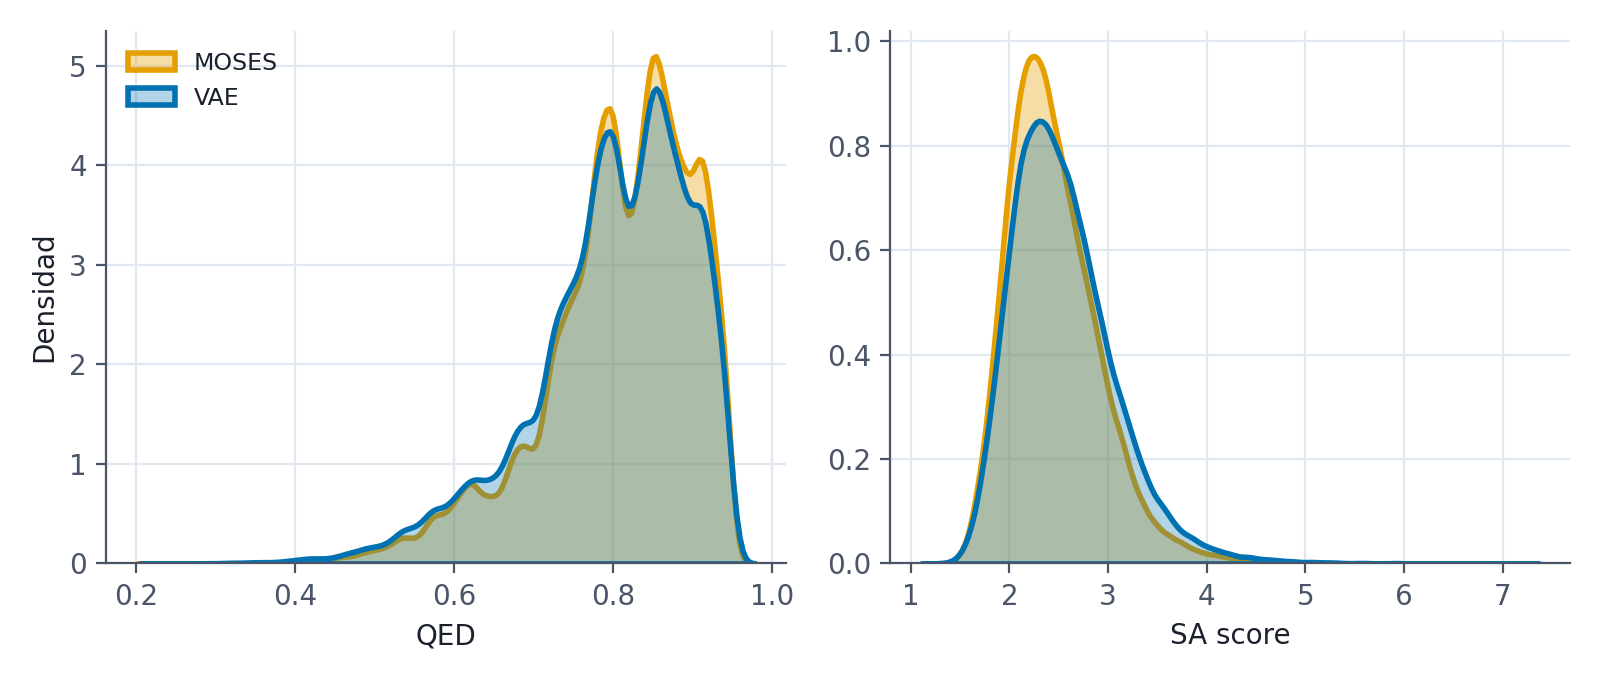
\includegraphics[width=0.8\textwidth]{Figures/distribuciones_qed_sa.png}
\caption{Distribuciones de QED y SAS de las moléculas válidas generadas por SM-L 2 frente al conjunto de prueba de MOSES.}
\label{fig:distribuciones}
\end{figure}

\begin{figure}[htbp]
\centering
\framebox[\textwidth]{\rule{0pt}{6cm}\textbf{[Placeholder: Figura 4.2 -- Muestras de moléculas generadas por el modelo SM-L 2]}}
\caption{Muestras de moléculas generadas por el modelo seleccionado SM-L 2.}
\label{fig:muestras_modelo_seleccionado}
\end{figure}


\subsubsection{Comparación con el estado del arte}

\begin{table}[htbp]
\centering
\caption{Comparación con el estado del arte utilizando el dataset MOSES}
\label{tab:resultados_reducidos}
\resizebox{\textwidth}{!}{%
\begin{tabular}{l c c c c c c c c}
\toprule
Model & Valid ($\uparrow$) & Unique ($\uparrow$) & Novelty ($\uparrow$) & Filters ($\uparrow$) & FCD ($\downarrow$) & IntDiv ($\uparrow$) & SA ($\downarrow$) & QED ($\downarrow$) \\
\midrule
Train & 1.000 & 1.000 & 1.000 & 1.000 & 0.008 & 0.857 & - & - \\
HMM & 0.076 & 0.567 & 0.999 & 0.902 & 24.466 & 0.847 & 0.742 & 0.269 \\
NGram & 0.238 & 0.922 & 0.969 & 0.958 & 5.507 & 0.874 & 0.231 & 0.089 \\
Combinatorial & 1.000 & 0.991 & 0.988 & 0.956 & 4.238 & 0.873 & 0.280 & 0.151 \\
CharRNN & 0.975 & 0.999 & 0.842 & 0.994 & 0.073 & 0.856 & 0.017 & 0.003 \\
AAE & 0.937 & 0.997 & 0.793 & 0.996 & 0.556 & 0.856 & 0.045 & 0.004 \\
LatentGAN & 0.897 & 0.997 & 0.950 & 0.974 & 0.297 & 0.857 & 0.088 & 0.006 \\
FRATTVAE & 1.000 & 1.000 & 0.974 & N/R & 0.865 & N/R & 2.591 & 0.030 \\
PCF-VAE & 0.980 & 1.000 & 0.938 & 0.990 & 0.296 & 0.859 & N/R & N/R \\
\textbf{SM-L VAE} & 0.962 & 1.000 & 0.943 & 0.988 & 0.179 & 0.859 & 0.093 & 0.008 \\
\bottomrule
\end{tabular}}
\end{table}

Los resultados indican que el modelo propuesto (SM-L VAE) ofrece un balance competitivo frente a otras arquitecturas recientes de espacio latente, como PCF-VAE y FRATTVAE. El modelo logra un \gls{fcd} de 0.179, manteniendo al mismo tiempo una alta tasa de novedad (0.943) y diversidad interna (0.859). Si bien enfoques autorregresivos como CharRNN alcanzan un \gls{fcd} numéricamente menor (0.073), este comportamiento suele estar asociado a una caída en la novedad (0.842), lo que sugiere una tendencia del modelo a replicar el conjunto de entrenamiento. La principal ventaja de los modelos \gls{vae} radica en su espacio latente continuo. A diferencia de las secuencias discretas de CharRNN, esta representación vectorial permite aplicar metaheurísticas multiobjetivo para buscar moléculas con propiedades específicas o afines a un target determinado.

\section{Optimización Multiobjetivo de Propiedades Moleculares sin Diana Específica}
\label{sec:res_genericos}

En esta sección se aborda la optimización multiobjetivo de propiedades moleculares sin diana específica mediante metaheurísticas en el espacio latente del \gls{vae}. Se describen los resultados del ajuste de hiperparámetros y la influencia de los operadores de cruce y mutación, para luego contrastar el desempeño global de los cinco algoritmos y caracterizar las moléculas candidatas obtenidas en el frente de Pareto conjunto.

\subsection{Ajuste de Hiperparámetros}
\label{subsec:res_metaheuristicas_hp}

Siguiendo el protocolo experimental establecido en la Sección~\ref{subsec:protocolo_ajuste}, la exploración de hiperparámetros se evaluó utilizando el hipervolumen (\acrshort{hv}) como métrica principal sobre 20 semillas independientes. La mejor configuración obtenida para cada algoritmo y combinación de operadores se detalla en el Apéndice~\ref{sec:apendice_hp_seleccionadas} (Tabla~\ref{tab:hp_seleccionadas}).

En términos generales, al evaluar los objetivos \gls{qed} y SA bajo la restricción de factibilidad ($F_{\text{sp3}} \ge 0.30$), los valores de hipervolumen se sitúan en el rango de $\sim 1.10\text{--}1.12$. Asimismo, la mayoría de las configuraciones seleccionadas favorece esquemas con mayor número de generaciones ($100\times 1000$ y $200\times 500$), lo cual permite una explotación más prolongada en el espacio latente frente a particiones de población más amplia ($400\times 250$). En \acrshort{cmopso}, la configuración seleccionada ($100\times 1000$, archivo élite de 10, velocidad $v_{\text{max}} = 0.1$ y mutación $0.031$) alcanza un hipervolumen medio de $1.1092$.

\subsubsection{Compromiso entre Hipervolumen y Validez Química}

La Figura~\ref{fig:hv_vs_val} muestra el compromiso entre hipervolumen y validez química en todas las configuraciones evaluadas (mediana de 20 semillas).

\begin{figure}[H]
    \centering
    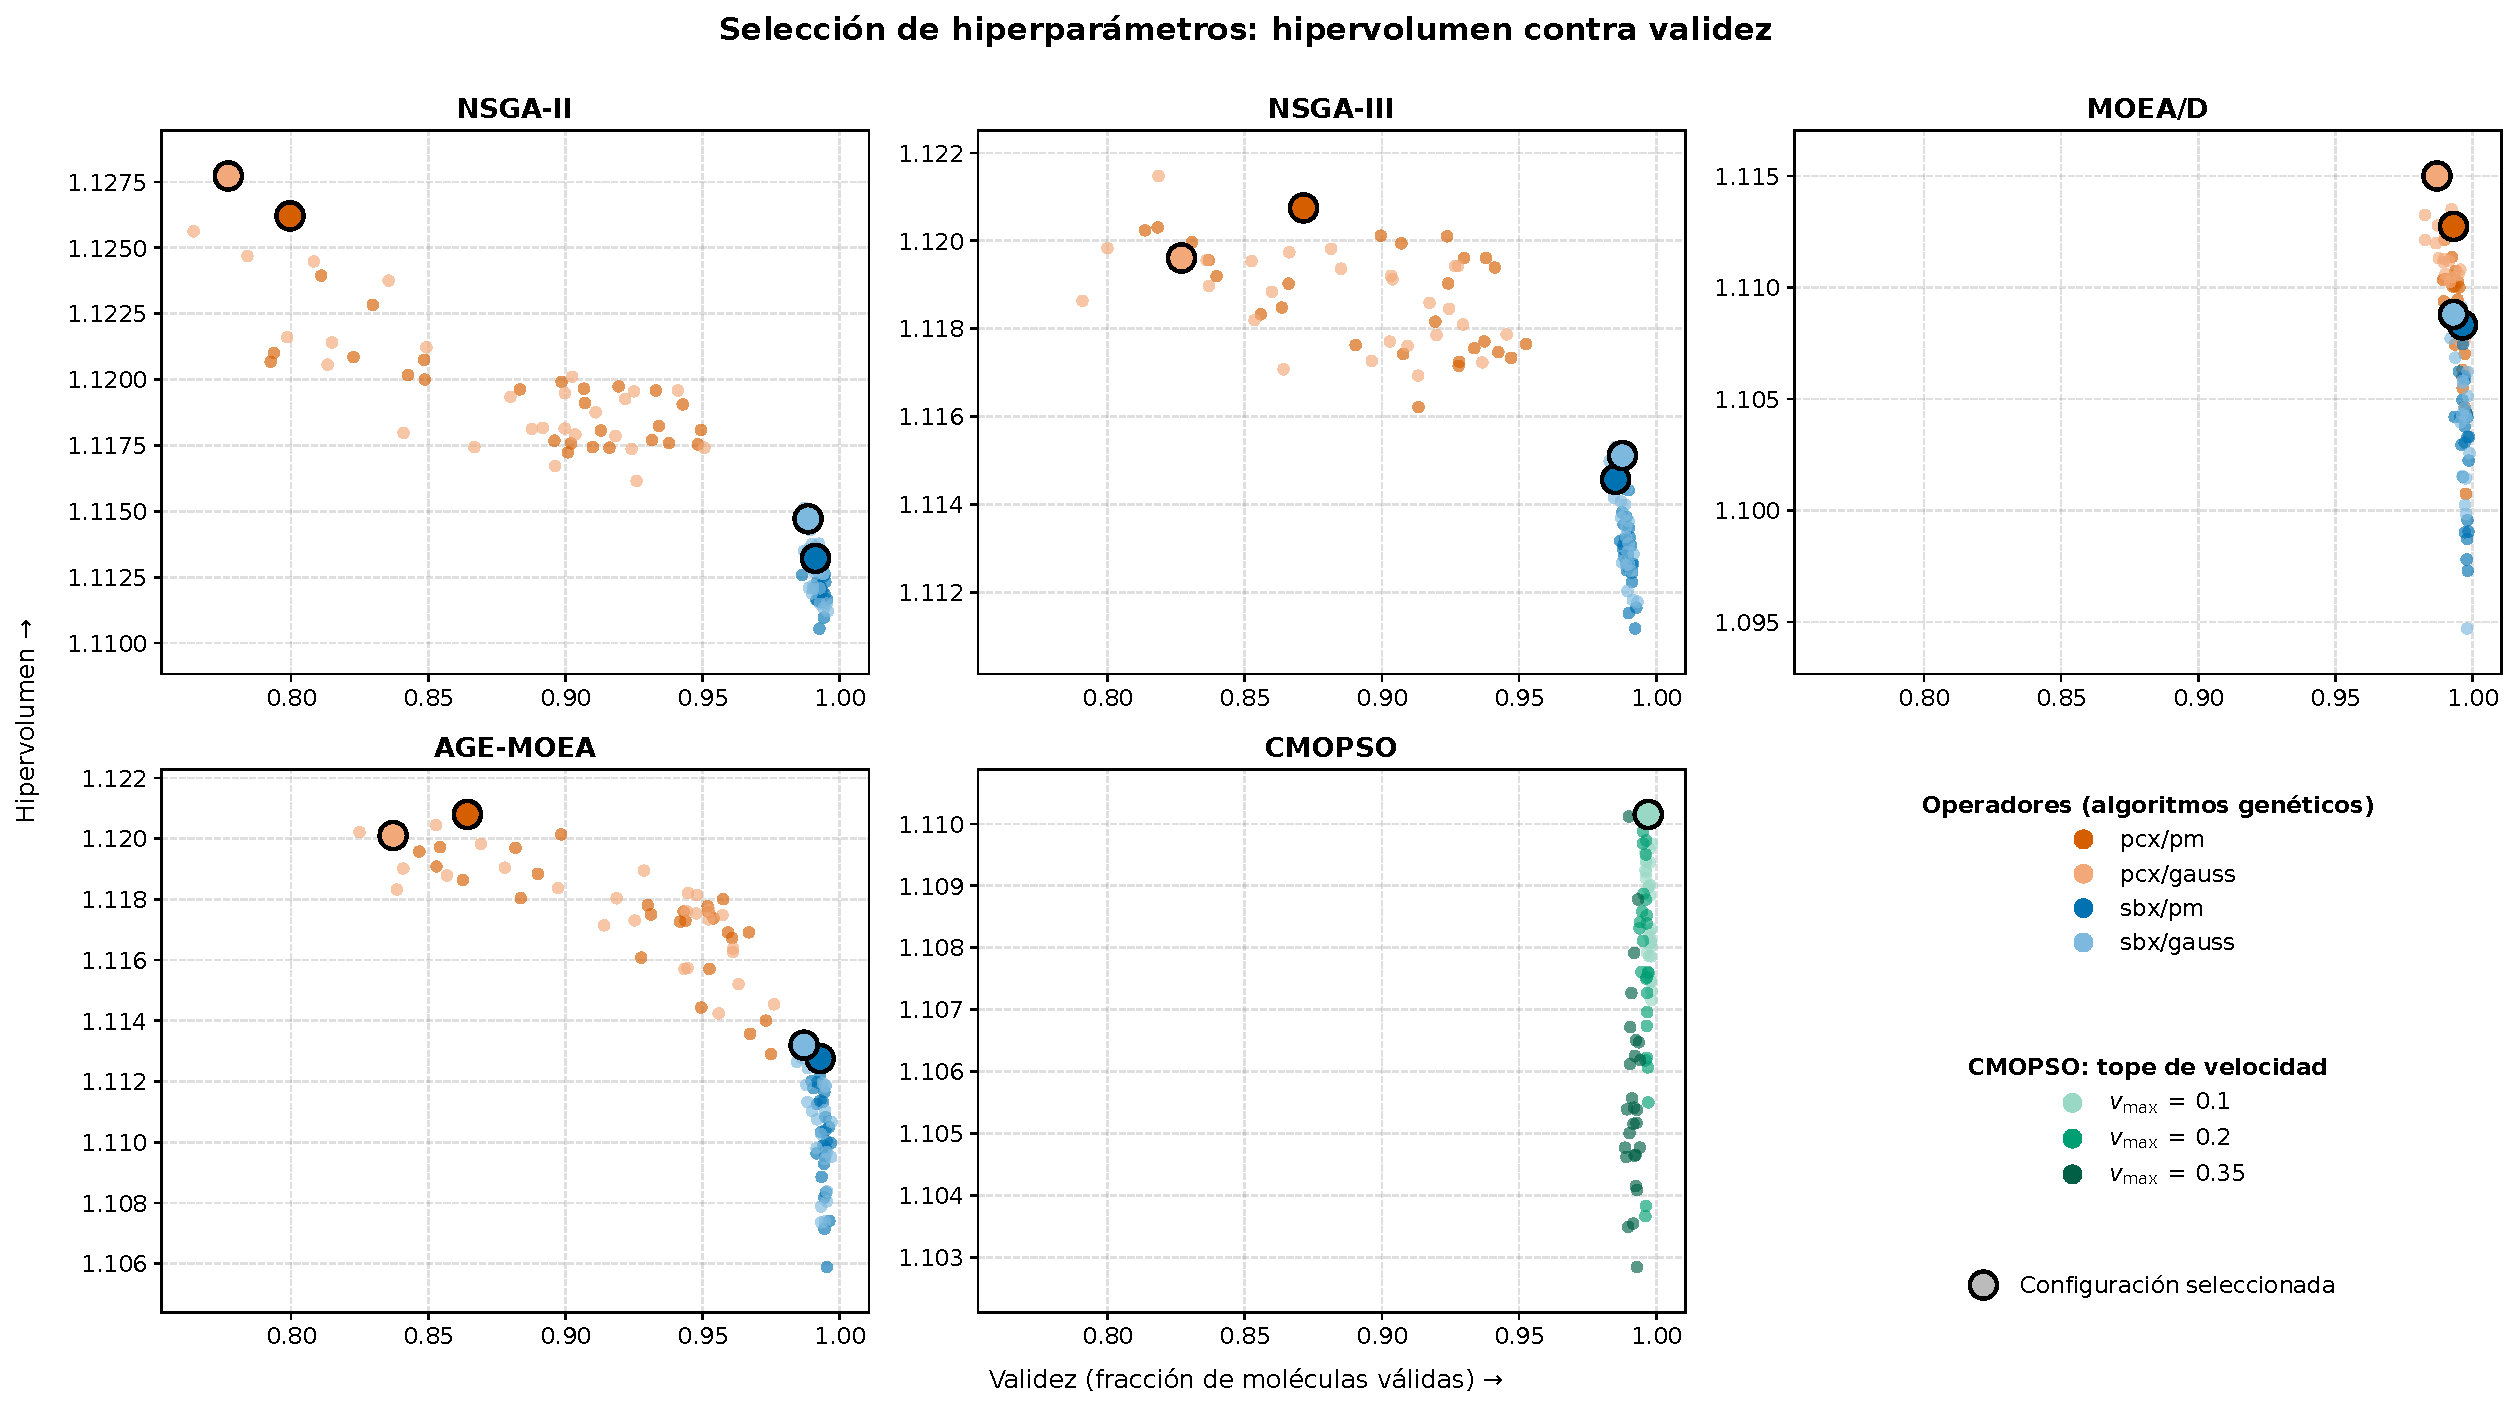
\includegraphics[width=\textwidth]{Figures/metaheuristicas/hp/hypervolume_vs_validity.pdf}
    \caption{Relación de compromiso entre Hipervolumen y Validez Química para todas las configuraciones evaluadas (mediana de 20 semillas). Con borde negro, la configuración seleccionada para cada combinación de operadores.}
    \label{fig:hv_vs_val}
\end{figure}

Este análisis muestra los siguientes comportamientos:
\begin{itemize}
    \item \textbf{Separación por operador de cruce:} En los algoritmos genéticos se aprecia una clara diferenciación según el operador de cruce. Las variantes con PCX logran los mayores valores de hipervolumen, a costa de una validez química moderada (entre $80\%$ y $95\%$). En contraposición, las variantes con SBX preservan una validez casi completa (entre $98\%$ y $100\%$), aunque con un hipervolumen inferior.
    \item \textbf{Alta validez en \acrshort{moead}:} \acrshort{moead} mantiene una validez química superior al $98\%$ en la totalidad de sus configuraciones, independientemente de los operadores empleados.
    \item \textbf{Comportamiento en \acrshort{cmopso}:} \acrshort{cmopso} presenta una validez superior al $99\%$ en prácticamente todas sus configuraciones. Su hipervolumen se encuentra fuertemente condicionado por el tope de velocidad: los valores bajos ($v_{\text{max}} = 0.1$) permiten alcanzar los mayores hipervolúmenes, mientras que un aumento en la velocidad ($v_{\text{max}} = 0.35$) produce un descenso apreciable del hipervolumen.
\end{itemize}

\begin{figure}[H]
    \centering
    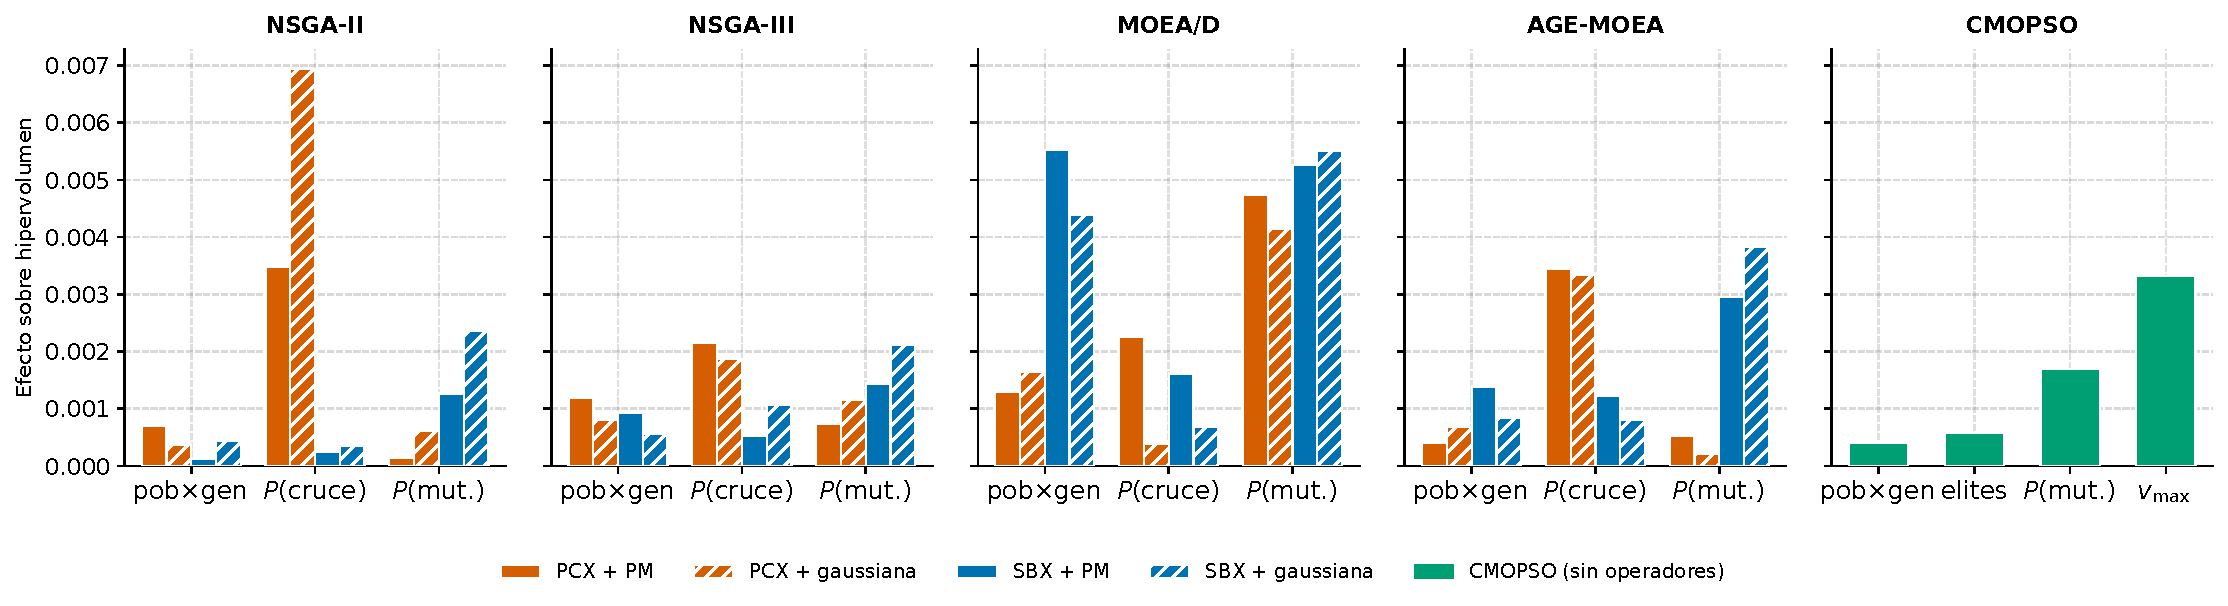
\includegraphics[width=\textwidth]{Figures/metaheuristicas/hp/efectos_hypervolume.pdf}
    \caption{Efecto de cada hiperparámetro sobre el hipervolumen dentro de cada combinación de operadores en los algoritmos genéticos y en \acrshort{cmopso}.}
    \label{fig:efectos_hypervolume}
\end{figure}

La Figura~\ref{fig:efectos_hypervolume} resume la magnitud del efecto de cada hiperparámetro sobre el hipervolumen. En los algoritmos genéticos, las variantes con PCX son predominantemente sensibles a la probabilidad de cruce $P(\text{cruce})$ (con un efecto especialmente marcado en \acrshort{nsga2}), mientras que las variantes con SBX responden principalmente a la probabilidad de mutación $P(\text{mut.})$. \acrshort{moead} exhibe una marcada sensibilidad tanto a la mutación como al reparto de población y generaciones. En \acrshort{cmopso}, el parámetro de mayor impacto es el tope de velocidad ($v_{\text{max}}$), seguido por la probabilidad de mutación, mientras que el tamaño del archivo de élites y la partición del presupuesto presentan una influencia secundaria.

\subsection{Influencia de los Operadores de Cruce y Mutación}
\label{subsec:comparativa_operadores}

Se evalúa el impacto de los operadores de cruce (SBX, PCX) y mutación (Polinomial, Gaussiana) en \acrshort{agemoea}, \acrshort{moead}, \acrshort{nsga2} y \acrshort{nsga3} sobre distintos indicadores multiobjetivo y químicos.

La comparación estadística se realiza sobre el hipervolumen: test de Friedman con las 20 semillas ($p < 0.001$), seguido de comparaciones por pares con Wilcoxon de rangos con signo y corrección de Holm ($\alpha = 0.05$). Para cada par se reporta el valor $p$ ajustado y la correlación rango-biserial de pares emparejados ($r_{\text{rb}}$), con signo positivo cuando la primera combinación aventaja a la segunda; un valor próximo al máximo ($\pm 1.0$) indica unanimidad en las 20 semillas.

\begin{table}[!htbp]
\centering
\caption{Comparación de indicadores multiobjetivo para las distintas combinaciones de operadores de cruce y mutación (media $\pm$ desviación estándar sobre 20 semillas independientes).}
\label{tab:comparison_multiobjective_operadores}%
\label{tab:comparison_multiobjective_agemoea}%
\label{tab:comparison_multiobjective_moead}%
\label{tab:comparison_multiobjective_nsga2}%
\label{tab:comparison_multiobjective_nsga3}
\setlength{\tabcolsep}{3.5pt}
\resizebox{\textwidth}{!}{%
\begin{tabular}{lcccccc}
\toprule
Operadores & \acrshort{hv} $\uparrow$ & Esp. $\downarrow$ & $\text{IGD}^+$ $\downarrow$ & $\epsilon^+$ $\downarrow$ & $|\mathcal{P}|$ $\uparrow$ & Tiempo (s) $\downarrow$ \\
\midrule
\multicolumn{7}{c}{\textbf{\acrshort{agemoea}}} \\
\cmidrule(lr){1-7}
PCX + PM & $1.121 \pm 0.003$ & $1.169 \pm 0.352$ & $0.040 \pm 0.005$ & $\mathbf{0.118 \pm 0.020}$ & $\mathbf{24.1 \pm 4.4}$ & $110.7 \pm 5.1$ \\
PCX + Gauss & $\mathbf{1.122 \pm 0.004}$ & $1.019 \pm 0.357$ & $\mathbf{0.037 \pm 0.007}$ & $0.119 \pm 0.029$ & $22.9 \pm 4.1$ & $120.2 \pm 4.5$ \\
SBX + PM & $1.113 \pm 0.002$ & $\mathbf{0.903 \pm 0.306}$ & $0.053 \pm 0.006$ & $0.180 \pm 0.022$ & $19.4 \pm 2.4$ & $229.6 \pm 19.6$ \\
SBX + Gauss & $1.114 \pm 0.003$ & $1.025 \pm 0.314$ & $0.052 \pm 0.009$ & $0.178 \pm 0.024$ & $18.2 \pm 3.9$ & $\mathbf{97.0 \pm 3.6}$ \\
\midrule
\multicolumn{7}{c}{\textbf{\acrshort{moead}}} \\
\cmidrule(lr){1-7}
PCX + PM & $1.113 \pm 0.004$ & $1.042 \pm 0.272$ & $0.057 \pm 0.011$ & $\mathbf{0.173 \pm 0.032}$ & $19.9 \pm 3.5$ & $43.9 \pm 2.4$ \\
PCX + Gauss & $\mathbf{1.114 \pm 0.003}$ & $1.112 \pm 0.383$ & $\mathbf{0.053 \pm 0.009}$ & $0.173 \pm 0.025$ & $\mathbf{19.9 \pm 4.1}$ & $52.2 \pm 3.0$ \\
SBX + PM & $1.107 \pm 0.005$ & $1.112 \pm 0.308$ & $0.068 \pm 0.014$ & $0.199 \pm 0.029$ & $17.9 \pm 3.7$ & $\mathbf{38.5 \pm 1.5}$ \\
SBX + Gauss & $1.108 \pm 0.006$ & $\mathbf{1.033 \pm 0.370}$ & $0.069 \pm 0.013$ & $0.199 \pm 0.024$ & $17.4 \pm 3.7$ & $41.4 \pm 2.5$ \\
\midrule
\multicolumn{7}{c}{\textbf{\acrshort{nsga2}}} \\
\cmidrule(lr){1-7}
PCX + PM & $1.125 \pm 0.004$ & $1.228 \pm 0.446$ & $0.038 \pm 0.006$ & $0.101 \pm 0.023$ & $\mathbf{29.4 \pm 4.7}$ & $99.0 \pm 4.1$ \\
PCX + Gauss & $\mathbf{1.126 \pm 0.005}$ & $1.264 \pm 0.502$ & $\mathbf{0.034 \pm 0.008}$ & $\mathbf{0.094 \pm 0.031}$ & $26.1 \pm 5.7$ & $102.2 \pm 4.7$ \\
SBX + PM & $1.114 \pm 0.002$ & $1.132 \pm 0.362$ & $0.051 \pm 0.005$ & $0.181 \pm 0.011$ & $24.0 \pm 3.9$ & $\mathbf{56.5 \pm 5.7}$ \\
SBX + Gauss & $1.116 \pm 0.003$ & $\mathbf{1.086 \pm 0.324}$ & $0.046 \pm 0.008$ & $0.167 \pm 0.023$ & $21.9 \pm 4.2$ & $59.4 \pm 4.4$ \\
\midrule
\multicolumn{7}{c}{\textbf{\acrshort{nsga3}}} \\
\cmidrule(lr){1-7}
PCX + PM & $\mathbf{1.121 \pm 0.003}$ & $1.171 \pm 0.390$ & $\mathbf{0.036 \pm 0.006}$ & $\mathbf{0.121 \pm 0.021}$ & $22.7 \pm 5.1$ & $108.3 \pm 3.7$ \\
PCX + Gauss & $1.121 \pm 0.004$ & $1.221 \pm 0.322$ & $0.038 \pm 0.005$ & $0.124 \pm 0.025$ & $23.8 \pm 4.2$ & $106.0 \pm 4.4$ \\
SBX + PM & $1.115 \pm 0.002$ & $\mathbf{1.130 \pm 0.314}$ & $0.048 \pm 0.005$ & $0.171 \pm 0.016$ & $\mathbf{24.8 \pm 3.4}$ & $\mathbf{60.5 \pm 4.0}$ \\
SBX + Gauss & $1.116 \pm 0.003$ & $1.137 \pm 0.467$ & $0.045 \pm 0.007$ & $0.163 \pm 0.024$ & $22.9 \pm 3.5$ & $64.8 \pm 6.1$ \\
\bottomrule
\end{tabular}%
}
\end{table}



La Tabla~\ref{tab:comparison_multiobjective_operadores} compara las configuraciones de \acrshort{agemoea}, \acrshort{moead}, \acrshort{nsga2} y \acrshort{nsga3} frente a las distintas combinaciones de operadores de cruce y mutación sobre indicadores de convergencia (\acrshort{hv}, $\text{IGD}^+$), cobertura ($\epsilon^+$), distribución (espaciamiento), tamaño del frente y costo computacional.

A nivel general, el factor determinante en el desempeño multiobjetivo es el operador de cruce, mientras que el impacto de la mutación (polinomial vs. gaussiana) resulta secundario. Las combinaciones basadas en PCX superan de forma sistemática a las de SBX en todos los algoritmos, alcanzando hipervolúmenes superiores ($\text{HV} \approx 1.113\text{--}1.126$ frente a $1.107\text{--}1.116$ en SBX) y una aproximación sustancialmente más cercana al frente de referencia (reducciones notorias en $\text{IGD}^+$ y $\epsilon^+$). Esta superioridad responde a la dinámica de exploración en el espacio latente continuo del \gls{vae}: mientras que SBX recombina únicamente dos progenitores coordenada a coordenada atrapando a la población en regiones intermedias conocidas, PCX proyecta descendientes a partir de una nube de múltiples padres, favoreciendo la dispersión hacia regiones extremas no exploradas. La contrapartida de esta búsqueda más amplia es un incremento en el tiempo de cómputo (por la mayor complejidad del muestreo) y un espaciamiento numéricamente superior, derivado de extender soluciones hacia los bordes del frente en lugar de concentrarlas densamente en el centro.

En \acrshort{nsga2}, la combinación con PCX alcanza el mejor desempeño global de la comparativa ($\text{HV} = 1.126$, $\epsilon^+ = 0.094$). Este algoritmo es el que mayor provecho obtiene de la dispersión de PCX, reflejado en el frente no dominado más numeroso ($29.4$ soluciones en promedio frente a $21.9\text{--}24.0$ en SBX). Esto se debe a su mecanismo de selección basado en la distancia de apiñamiento (\textit{crowding distance}), el cual recompensa a las soluciones aisladas generadas en los bordes y permite retener un abanico continuo de alternativas que abarca desde compuestos de máxima facilidad de síntesis hasta moléculas de alto \gls{qed}.

En \acrshort{nsga3}, las variantes con PCX logran una convergencia sobresaliente ($\text{IGD}^+ = 0.036$, el valor más bajo de la comparativa) y un \acrshort{hv} de $1.121$. A diferencia de \acrshort{nsga2}, el tamaño del frente se mantiene prácticamente invariable entre configuraciones ($22.7\text{--}24.8$ soluciones). Este comportamiento responde a la sustitución de la distancia de apiñamiento por puntos de referencia estructurados en un hiperplano, lo que acota la acumulación de soluciones en los extremos y preserva una distribución espacial uniforme a lo largo del frente independientemente de la agresividad del operador de cruce.

En \acrshort{agemoea}, el uso de PCX consolida un frente competitivo ($\text{HV} = 1.122$ e $\text{IGD}^+ = 0.037$ en pcx\_gauss) con un conjunto amplio de soluciones ($24.1$ en pcx\_pm). No obstante, el algoritmo acusa una marcada sensibilidad computacional según el operador empleado: la variante \texttt{sbx\_pm} eleva el tiempo a $229.6$~s frente a los $\approx 97\text{--}120$~s de las restantes configuraciones. Esta sobrecarga sugiere que la combinación de un cruce concentrador con mutación polinomial dificulta el ajuste adaptativo de la geometría del frente que realiza \acrshort{agemoea}, requiriendo mayor iteración en el cálculo de distancias extremas de supervivencia.

Por último, \acrshort{moead} presenta la menor brecha relativa entre familias de cruce y registra los menores tiempos de ejecución ($38.5\text{--}52.2$~s) y espaciamientos más reducidos ($1.033\text{--}1.042$). Al descomponer la búsqueda en subproblemas escalares acotados a vecindarios locales fijos, la capacidad de dispersión de PCX queda parcialmente restringida al entorno de soluciones vecinas muy similares entre sí. En consecuencia, aunque PCX mejora la cobertura frente a SBX, la dinámica de vecindad de \acrshort{moead} prioriza la explotación local, evitando que el frente se expanda hacia los extremos del espacio de propiedades.

\begin{table}[!htbp]
\centering
\caption{Comparación de indicadores químicos para las distintas combinaciones de operadores de cruce y mutación (media $\pm$ desviación estándar sobre 20 semillas independientes).}
\label{tab:comparison_chemical_operadores}%
\label{tab:comparison_chemical_agemoea}%
\label{tab:comparison_chemical_moead}%
\label{tab:comparison_chemical_nsga2}%
\label{tab:comparison_chemical_nsga3}
\setlength{\tabcolsep}{3.5pt}
\resizebox{\textwidth}{!}{%
\begin{tabular}{lccccccc}
\toprule
Operadores & QED $\uparrow$ & SA $\downarrow$ & Fact. $\uparrow$ & $F_{\text{sp3}}$ & Val. $\uparrow$ & Uni. $\uparrow$ & Nov. $\uparrow$ \\
\midrule
\multicolumn{8}{c}{\textbf{\acrshort{agemoea}}} \\
\cmidrule(lr){1-8}
PCX + PM & $0.848 \pm 0.040$ & $1.620 \pm 0.090$ & $0.746 \pm 0.038$ & $0.413 \pm 0.041$ & $0.864 \pm 0.026$ & $0.986 \pm 0.022$ & $0.974 \pm 0.007$ \\
PCX + Gauss & $0.848 \pm 0.054$ & $1.620 \pm 0.080$ & $0.736 \pm 0.035$ & $0.408 \pm 0.058$ & $0.831 \pm 0.038$ & $\mathbf{0.998 \pm 0.005}$ & $\mathbf{0.977 \pm 0.006}$ \\
SBX + PM & $\mathbf{0.884 \pm 0.010}$ & $\mathbf{1.610 \pm 0.060}$ & $\mathbf{0.859 \pm 0.044}$ & $0.390 \pm 0.017$ & $\mathbf{0.990 \pm 0.010}$ & $0.323 \pm 0.033$ & $0.624 \pm 0.208$ \\
SBX + Gauss & $0.884 \pm 0.013$ & $1.630 \pm 0.080$ & $0.856 \pm 0.052$ & $0.384 \pm 0.026$ & $0.984 \pm 0.011$ & $0.483 \pm 0.067$ & $0.696 \pm 0.167$ \\
\midrule
\multicolumn{8}{c}{\textbf{\acrshort{moead}}} \\
\cmidrule(lr){1-8}
PCX + PM & $0.877 \pm 0.017$ & $1.660 \pm 0.070$ & $0.882 \pm 0.050$ & $0.388 \pm 0.020$ & $0.991 \pm 0.005$ & $0.445 \pm 0.070$ & $0.745 \pm 0.091$ \\
PCX + Gauss & $0.882 \pm 0.015$ & $\mathbf{1.650 \pm 0.080}$ & $0.875 \pm 0.044$ & $0.387 \pm 0.032$ & $0.985 \pm 0.009$ & $\mathbf{0.545 \pm 0.060}$ & $\mathbf{0.793 \pm 0.066}$ \\
SBX + PM & $\mathbf{0.889 \pm 0.012}$ & $1.700 \pm 0.050$ & $\mathbf{0.930 \pm 0.030}$ & $0.391 \pm 0.024$ & $\mathbf{0.997 \pm 0.001}$ & $0.255 \pm 0.048$ & $0.700 \pm 0.104$ \\
SBX + Gauss & $0.884 \pm 0.017$ & $1.690 \pm 0.090$ & $0.923 \pm 0.031$ & $0.407 \pm 0.033$ & $0.990 \pm 0.009$ & $0.380 \pm 0.060$ & $0.740 \pm 0.181$ \\
\midrule
\multicolumn{8}{c}{\textbf{\acrshort{nsga2}}} \\
\cmidrule(lr){1-8}
PCX + PM & $0.803 \pm 0.058$ & $1.620 \pm 0.080$ & $0.735 \pm 0.023$ & $0.464 \pm 0.064$ & $0.798 \pm 0.036$ & $0.991 \pm 0.010$ & $0.983 \pm 0.003$ \\
PCX + Gauss & $0.805 \pm 0.067$ & $\mathbf{1.580 \pm 0.080}$ & $0.746 \pm 0.036$ & $0.458 \pm 0.076$ & $0.786 \pm 0.033$ & $\mathbf{0.996 \pm 0.008}$ & $\mathbf{0.983 \pm 0.005}$ \\
SBX + PM & $\mathbf{0.889 \pm 0.014}$ & $1.650 \pm 0.080$ & $\mathbf{0.867 \pm 0.029}$ & $0.397 \pm 0.032$ & $\mathbf{0.989 \pm 0.006}$ & $0.833 \pm 0.048$ & $0.804 \pm 0.045$ \\
SBX + Gauss & $0.884 \pm 0.014$ & $1.630 \pm 0.100$ & $0.857 \pm 0.037$ & $0.389 \pm 0.031$ & $0.988 \pm 0.006$ & $0.761 \pm 0.077$ & $0.847 \pm 0.043$ \\
\midrule
\multicolumn{8}{c}{\textbf{\acrshort{nsga3}}} \\
\cmidrule(lr){1-8}
PCX + PM & $0.854 \pm 0.044$ & $\mathbf{1.600 \pm 0.090}$ & $0.744 \pm 0.042$ & $0.408 \pm 0.049$ & $0.863 \pm 0.036$ & $\mathbf{0.999 \pm 0.003}$ & $0.973 \pm 0.007$ \\
PCX + Gauss & $0.851 \pm 0.060$ & $1.650 \pm 0.090$ & $0.747 \pm 0.038$ & $0.415 \pm 0.072$ & $0.826 \pm 0.041$ & $0.998 \pm 0.005$ & $\mathbf{0.980 \pm 0.005}$ \\
SBX + PM & $\mathbf{0.885 \pm 0.008}$ & $1.610 \pm 0.060$ & $0.819 \pm 0.025$ & $0.408 \pm 0.021$ & $\mathbf{0.985 \pm 0.004}$ & $0.756 \pm 0.044$ & $0.824 \pm 0.034$ \\
SBX + Gauss & $0.881 \pm 0.011$ & $1.620 \pm 0.080$ & $\mathbf{0.841 \pm 0.030}$ & $0.392 \pm 0.027$ & $0.985 \pm 0.008$ & $0.853 \pm 0.057$ & $0.843 \pm 0.028$ \\
\bottomrule
\end{tabular}%
}
\end{table}



La Tabla~\ref{tab:comparison_chemical_operadores} resume las propiedades químicas obtenidas para los cuatro algoritmos, donde \gls{qed} y SA se promedian sobre el frente no dominado acumulado, la validez, factibilidad y novedad sobre el total de evaluaciones de la ejecución, la unicidad sobre la población final, y $F_{\text{sp3}}$ como nivel medio de saturación alcanzado bajo la restricción.

A nivel general, las propiedades químicas exhiben un compromiso directo condicionado por el operador de cruce. Las variantes con SBX generan descendientes en la vecindad inmediata de los progenitores, manteniéndose en regiones densas y confiables del modelo generativo; esto asegura una validez química sobresaliente ($> 98\%$) y una alta tasa de factibilidad ($82\%\text{--}93\%$), pero a costa de una pérdida apreciable de diversidad estructural, reflejada en menores niveles de unicidad y novedad por la reiteración de análogos ya conocidos en el entrenamiento. En contraposición, PCX aplica perturbaciones direccionales basadas en múltiples progenitores hacia zonas menos densas del espacio latente, lo que permite preservar una elevada unicidad y novedad ($>97\%$ en la mayoría de los métodos) junto con una mayor tridimensionalidad ($F_{\text{sp3}} \ge 0.38$), asumiendo una reducción moderada en la validez ($78\%\text{--}86\%$). Cabe destacar que en todas las variantes evaluadas la accesibilidad sintética media se mantiene en rangos favorables ($\text{SA} \approx 1.58\text{--}1.70$), confirmando que la mayor exploración de PCX no degrada la viabilidad sintética de los candidatos generados.

En \acrshort{nsga2}, las combinaciones con PCX destacan por alcanzar la mayor diferenciación química, registrando una novedad superior al $98\%$ frente a los compuestos de entrenamiento y un $F_{\text{sp3}}$ medio de $0.46$, el más elevado entre todos los algoritmos evaluados, lo que asegura un marcado carácter tridimensional bajo la restricción impuesta ($F_{\text{sp3}} \ge 0.30$) junto con un SA favorable de $1.58\text{--}1.62$. Su validez química desciende a $78.6\%\text{--}79.8\%$, con una factibilidad del $73.5\%\text{--}74.6\%$. Si bien las variantes con SBX obtienen mayor validez ($> 98.7\%$) y un \gls{qed} promedio superior ($0.884\text{--}0.889$ frente a $0.803\text{--}0.805$ en PCX), esto se debe a que concentran su búsqueda en un tramo acotado de alta similitud, mientras que PCX expande el espacio explorado hacia candidatos con andamiajes no reportados. En cuanto a la mutación, su efecto resulta secundario frente al cruce, aunque la mutación gaussiana en SBX aporta una novedad algo superior ($84.7\%$ frente a $80.4\%$ con polinomial).

En \acrshort{nsga3}, las combinaciones con PCX preservan la mayor diversidad en la población final, alcanzando una unicidad prácticamente perfecta ($\ge 99.8\%$) y una novedad de $97.3\%\text{--}98.0\%$, junto con un $F_{\text{sp3}}$ medio de $0.41$ y un SA favorable de $1.60\text{--}1.65$. Su validez química se sitúa entre $82.6\%$ y $86.3\%$, con una factibilidad del $74.4\%\text{--}74.7\%$. En cambio, SBX obtiene un \gls{qed} promedio superior ($0.881\text{--}0.885$ frente a $0.851\text{--}0.854$ en PCX), mayor validez ($> 98.4\%$) y mayor factibilidad ($81.9\%\text{--}84.1\%$), pero su menor dispersión reduce la unicidad ($75.6\%$ en \texttt{sbx\_pm} y $85.3\%$ en \texttt{sbx\_gauss}) y la novedad ($82.4\%\text{--}84.3\%$), mostrando mayor repetición de estructuras. La mutación muestra un efecto secundario frente al cruce, registrando una validez algo mayor con mutación polinomial en PCX ($86.3\%$ frente a $82.6\%$ con gaussiana).

En \acrshort{agemoea}, se observa la caída más marcada de diversidad bajo SBX, donde la unicidad de la población final se reduce al $32.3\%\text{--}48.3\%$ y la novedad desciende a $62.4\%\text{--}69.6\%$, lo que en la práctica representa una desventaja al generar estructuras repetidas. En contraste, las combinaciones con PCX restablecen la variedad estructural, manteniendo una unicidad y novedad elevadas ($>97\%$), con un nivel de factibilidad en torno al $74\%$, una validez moderada ($83.1\%\text{--}86.4\%$) y un $F_{\text{sp3}}$ medio de $0.41$. Esto evidencia que la selección por geometría adaptativa de \acrshort{agemoea} requiere la diversidad que aporta PCX para no concentrarse prematuramente en familias moleculares análogas.

Por último, todas las configuraciones de \acrshort{moead} destacan por sostener una validez química alta ($> 98.4\%$) y una factibilidad de $87.5\%\text{--}93.0\%$, con valores de SA favorables ($1.65\text{--}1.70$) y un $F_{\text{sp3}}$ medio de $0.39\text{--}0.41$. No obstante, a diferencia de los otros métodos, en \acrshort{moead} la descomposición en subproblemas escalares y el cruce acotado a vecinos locales restringe la dispersión de PCX; en consecuencia, aun con este operador, la unicidad ($44.5\%\text{--}54.5\%$) y la novedad ($74.5\%\text{--}79.3\%$) resultan inferiores a las de los restantes algoritmos genéticos, concentrando la exploración en análogos moleculares conocidos.

Las pruebas de Wilcoxon de rangos con signo con corrección de Holm (detalladas en las Tablas~\ref{tab:ops_agemoea}, \ref{tab:ops_moead}, \ref{tab:ops_nsga2} y \ref{tab:ops_nsga3} del Apéndice~\ref{apendice:wilcoxon}) confirman que las combinaciones basadas en PCX superan a las de SBX en hipervolumen con significancia estadística en los cuatro algoritmos. Dentro de cada familia de cruce, el tipo de mutación (polinomial o gaussiana) no produce diferencias significativas en \acrshort{agemoea}, \acrshort{moead} ni \acrshort{nsga3}, definiendo. La única excepción se presenta en \acrshort{nsga2} bajo SBX, donde la mutación gaussiana supera de forma estadísticamente significativa a la polinomial.

\begin{figure}[H]
    \centering
    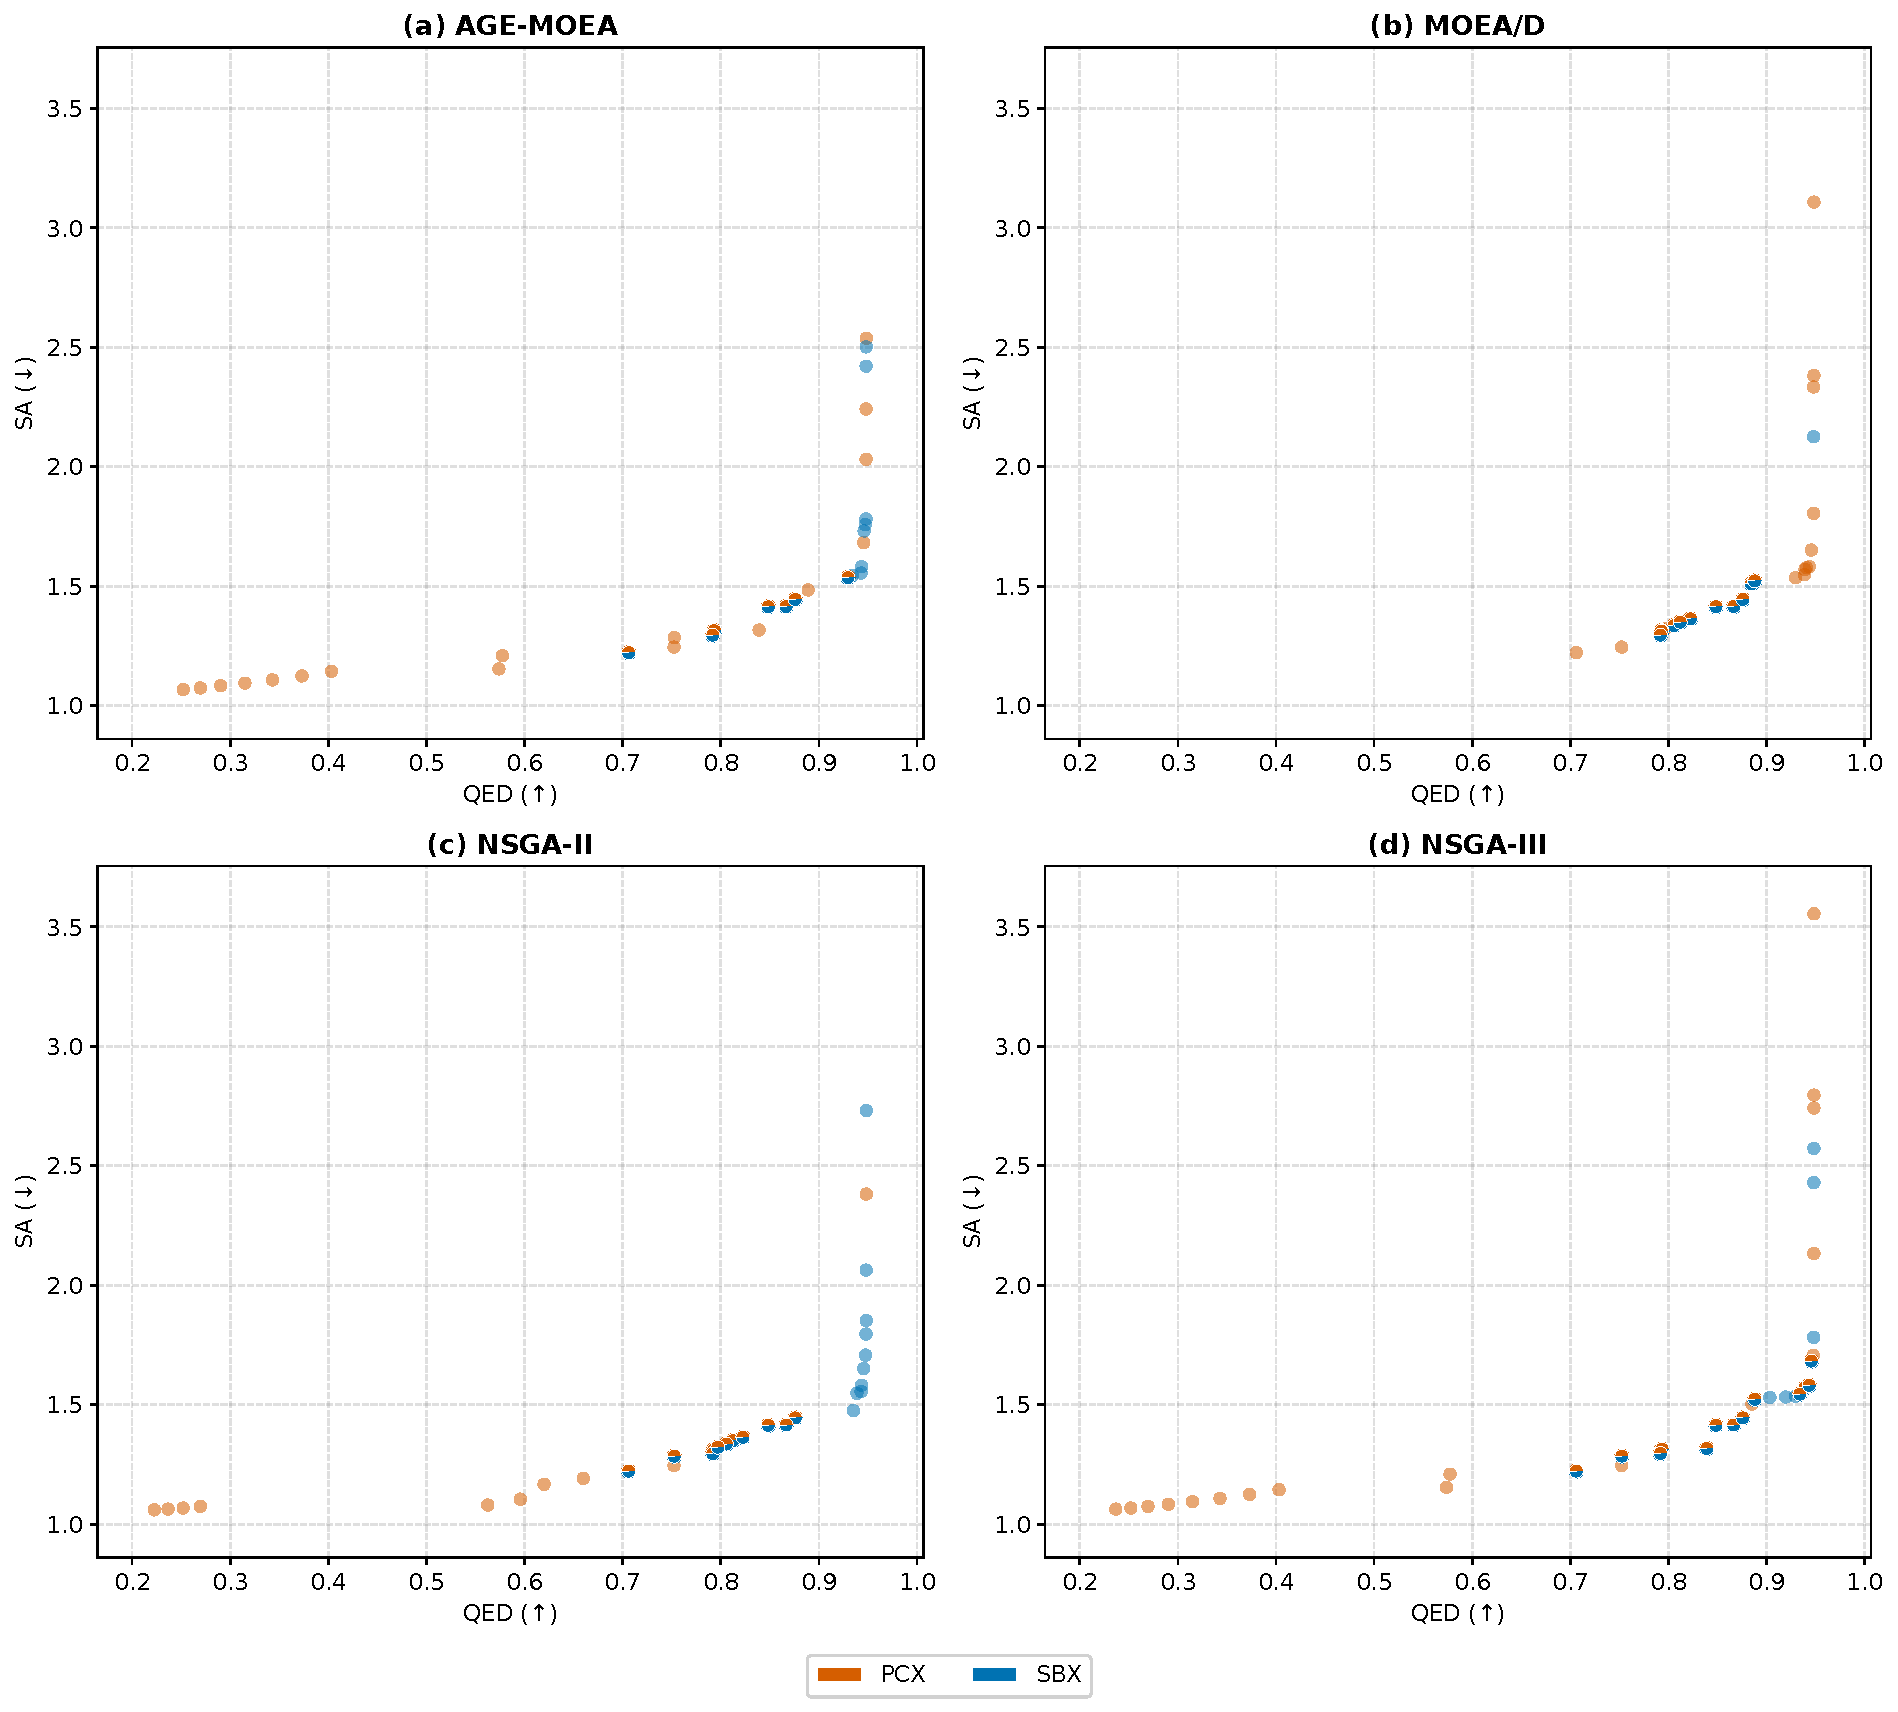
\includegraphics[width=\textwidth]{Figures/metaheuristicas/operadores/frente_conjunto_operadores.pdf}
    \caption{Frente no dominado conjunto por familia de cruce (PCX vs. SBX) para cada metaheurística: (a)~\acrshort{agemoea}, (b)~\acrshort{moead}, (c)~\acrshort{nsga2} y (d)~\acrshort{nsga3}.}
    \label{fig:frente_conjunto_operadores}
\end{figure}

La Figura~\ref{fig:frente_conjunto_operadores} muestra los frentes no dominados combinados de ambas familias de cruce en el espacio \gls{qed}--SA. Se observa una complementariedad clara entre los operadores: en la zona intermedia (\gls{qed} entre $0.80$ y $0.88$), donde coinciden la mayoría de las corridas (véanse las distribuciones por semilla en las Figuras~\ref{fig:pareto_agemoea_grid_nruns}--\ref{fig:pareto_nsga3_grid_nruns} del Apéndice~\ref{sec:apendice_frentes_nruns}), ambos operadores encuentran soluciones similares. La diferencia aparece en los extremos: PCX cubre en solitario la zona de menor SA ($\text{SA} \approx 1.06\text{--}1.20$), mientras que SBX aporta más soluciones en el tramo de alto \gls{qed} ($\approx 0.948$), donde la complejidad de las moléculas aumenta ($\text{SA} > 2.5$).

Entre los algoritmos, \acrshort{nsga2} y \acrshort{nsga3} logran los frentes más amplios, cubriendo tanto valores bajos de SA como altos de \gls{qed}. En \acrshort{agemoea}, PCX permite alcanzar la zona de bajo SA que SBX no logra explorar. En cambio, en \acrshort{moead} ambos operadores se quedan en valores de $\text{QED} > 0.70$ debido a la búsqueda por vecindarios, sin llegar al extremo de bajo SA.

En cuanto a las moléculas obtenidas (que se muestran en detalle en las Figuras~\ref{fig:moleculas_operadores_agemoea}--\ref{fig:moleculas_operadores_nsga3} del Apéndice~\ref{sec:apendice_moleculas_operadores}), todas las configuraciones alcanzan valores de \gls{qed} cercanos a $0.948$ con $\text{SA} < 3$. Con SBX predominan estructuras planas y sencillas, mientras que PCX incorpora más anillos no aromáticos, lo que aumenta la tridimensionalidad ($F_{\text{sp3}}$ de hasta $0.50$) manteniendo una adecuada facilidad de síntesis.

\subsection{Comparación Global de Metaheurísticas}
\label{subsec:comparacion_final}
\label{subsec:calidad_gen_moleculas}

En esta sección se comparan los cinco algoritmos (\acrshort{nsga2}, \acrshort{nsga3}, \acrshort{moead}, \acrshort{agemoea} y \acrshort{cmopso}) seleccionando la mejor configuración de cada uno a partir del estudio de hiperparámetros y operadores presentado anteriormente. Los cuatro algoritmos genéticos (\acrshort{nsga2}, \acrshort{nsga3}, \acrshort{moead} y \acrshort{agemoea}) emplean la combinación pcx\_pm, acorde a las comparaciones de la Sección~\ref{subsec:comparativa_operadores}. \acrshort{cmopso} usa su configuración de hiperparámetros ganadora ($100\times 1000$, $\text{élite}=10$, $p_m=0.031$, $v_{\text{max}}=0.1$).

\subsubsection{Indicadores Multiobjetivo y Químicos}

\begin{table}[H]
\centering
\rowcolors{2}{gray!10}{white}
\caption{Comparación de indicadores multiobjetivo - mejores configuraciones.}
\label{tab:comparison_multiobjective}
\resizebox{\textwidth}{!}{%
\begin{tabular}{lcccccc}
\toprule
Algoritmo & Hipervolumen $\uparrow$ & Espaciamiento $\downarrow$ & $\text{IGD}^+$ $\downarrow$ & $\epsilon^+$ $\downarrow$ & Tamaño de Pareto $\uparrow$ & Tiempo (s) $\downarrow$ \\
\midrule
\acrshort{nsga2} (PCX+PM) & $\mathbf{1.125 \pm 0.004}$ & $1.228 \pm 0.446$ & $0.038 \pm 0.006$ & $\mathbf{0.101 \pm 0.023}$ & $\mathbf{29.4 \pm 4.7}$ & $99.0 \pm 4.1$ \\
\acrshort{nsga3} (PCX+PM) & $1.121 \pm 0.003$ & $1.171 \pm 0.390$ & $\mathbf{0.036 \pm 0.006}$ & $0.121 \pm 0.021$ & $22.7 \pm 5.1$ & $108.3 \pm 3.7$ \\
\acrshort{moead} (PCX+PM) & $1.113 \pm 0.004$ & $\mathbf{1.042 \pm 0.272}$ & $0.057 \pm 0.011$ & $0.173 \pm 0.032$ & $19.9 \pm 3.5$ & $\mathbf{43.9 \pm 2.4}$ \\
\acrshort{agemoea} (PCX+PM) & $1.121 \pm 0.003$ & $1.170 \pm 0.352$ & $0.040 \pm 0.005$ & $0.118 \pm 0.020$ & $24.1 \pm 4.4$ & $110.7 \pm 5.1$ \\
\acrshort{cmopso} ($v_{\max}=0.1$) & $1.109 \pm 0.004$ & $1.053 \pm 0.380$ & $0.059 \pm 0.003$ & $0.191 \pm 0.011$ & $17.8 \pm 3.4$ & $50.2 \pm 1.9$ \\
\bottomrule
\end{tabular}%
}
\end{table}

La Tabla~\ref{tab:comparison_multiobjective} presenta la comparación de las mejores configuraciones de los cinco algoritmos en el espacio multiobjetivo. Se evalúan indicadores de convergencia y proximidad al frente de referencia (hipervolumen, $\text{IGD}^+$ y $\epsilon^+$), junto con la distribución (espaciamiento), el número de soluciones no dominadas factibles y el tiempo de ejecución.

Los resultados muestran que \acrshort{nsga2} alcanza el mayor hipervolumen promedio ($1.125$), el menor $\epsilon^+$ ($0.101$) y el frente más numeroso ($29.4$ soluciones factibles), y \acrshort{nsga3} el menor $\text{IGD}^+$ ($0.036$). \acrshort{nsga3} ($1.121$) y \acrshort{agemoea} ($1.121$) se ubican en un segundo nivel muy cercano en convergencia, con valores de $\text{IGD}^+$ de $0.036$ y $0.040$, $\epsilon^+$ de $0.121$ y $0.118$, y tamaños de frente de $22.7$ y $24.1$ soluciones, respectivamente. Por su parte, \acrshort{moead} ($1.113$) y \acrshort{cmopso} ($1.109$) obtienen hipervolúmenes menores y valores más altos en $\text{IGD}^+$ ($0.057$ y $0.059$) y $\epsilon^+$ ($0.173$ y $0.191$), lo que refleja que dejan segmentos del frente de referencia sin cubrir. No obstante, ambos destacan por una ejecución más rápida ($43.9$~s y $50.2$~s frente a $99.0\text{--}110.7$~s en los demás métodos) y por un espaciamiento menor ($1.042$ y $1.053$) al concentrar sus soluciones en la región de alto \gls{qed}.

Estas diferencias podrían deberse a cómo busca y selecciona cada algoritmo. En \acrshort{nsga2}, la distancia de apiñamiento permite que las soluciones se expandan libremente hacia los extremos del frente, lo que junto con PCX facilita descubrir moléculas tanto de bajo SA como de alto \gls{qed} y acumular más soluciones no dominadas. En cambio, \acrshort{cmopso} mueve sus partículas hacia las mejores soluciones encontradas, las cuales suelen concentrarse en la zona de alto \gls{qed}, lo que reduce la exploración hacia otras regiones. En \acrshort{moead}, cruzar únicamente entre vecinos cercanos favorece la búsqueda local pero limita la dispersión. Finalmente, \acrshort{nsga3} y \acrshort{agemoea} reparten las soluciones de forma más uniforme a lo largo del frente, logrando una buena convergencia sin acumular tantas moléculas como \acrshort{nsga2}.

\begin{table}[H]
\centering
\rowcolors{2}{gray!10}{white}
\caption{Comparación de indicadores químicos - mejores configuraciones.}
\label{tab:comparison_chemical}
\resizebox{\textwidth}{!}{%
\begin{tabular}{lccccccc}
\toprule
Algoritmo & QED $\uparrow$ & SA $\downarrow$ & Factibilidad $\uparrow$ & $F_{\text{sp3}}$ & Validez $\uparrow$ & Unicidad $\uparrow$ & Novedad $\uparrow$ \\
\midrule
\acrshort{nsga2} (PCX+PM) & $0.803 \pm 0.058$ & $1.620 \pm 0.080$ & $0.735 \pm 0.023$ & $0.464 \pm 0.064$ & $0.798 \pm 0.036$ & $0.991 \pm 0.010$ & $\mathbf{0.983 \pm 0.003}$ \\
\acrshort{nsga3} (PCX+PM) & $0.854 \pm 0.044$ & $\mathbf{1.600 \pm 0.090}$ & $0.744 \pm 0.042$ & $0.408 \pm 0.049$ & $0.863 \pm 0.036$ & $\mathbf{0.999 \pm 0.003}$ & $0.973 \pm 0.007$ \\
\acrshort{moead} (PCX+PM) & $0.877 \pm 0.017$ & $1.660 \pm 0.070$ & $0.882 \pm 0.050$ & $0.388 \pm 0.020$ & $0.991 \pm 0.005$ & $0.445 \pm 0.070$ & $0.745 \pm 0.091$ \\
\acrshort{agemoea} (PCX+PM) & $0.848 \pm 0.040$ & $1.620 \pm 0.090$ & $0.746 \pm 0.038$ & $0.413 \pm 0.041$ & $0.864 \pm 0.026$ & $0.986 \pm 0.022$ & $0.974 \pm 0.007$ \\
\acrshort{cmopso} ($v_{\max}=0.1$) & $\mathbf{0.887 \pm 0.009}$ & $1.650 \pm 0.080$ & $\mathbf{0.930 \pm 0.025}$ & $0.407 \pm 0.030$ & $\mathbf{0.996 \pm 0.005}$ & $0.320 \pm 0.064$ & $0.665 \pm 0.211$ \\
\bottomrule
\end{tabular}%
}
\end{table}


La Tabla~\ref{tab:comparison_chemical} presenta la comparación de las propiedades químicas entre los cinco algoritmos. \gls{qed} y SA se promedian sobre el frente no dominado acumulado, mientras que validez, factibilidad, unicidad, novedad y $F_{\text{sp3}}$ describen el comportamiento de la búsqueda sobre el espacio químico.

Los resultados dividen a los algoritmos en dos grupos definidos. Por un lado, \acrshort{cmopso} y \acrshort{moead} obtienen los valores promedio más altos de \gls{qed} ($0.887$ y $0.877$), junto con una validez química cercana al $100\%$. Sin embargo, este comportamiento reduce la diversidad de la población final, registrando una unicidad baja ($32.0\%$ en \acrshort{cmopso} y $44.5\%$ en \acrshort{moead}) y menor novedad frente a los compuestos de entrenamiento ($66.5\%$ y $74.5\%$).

Por otro lado, \acrshort{nsga2}, \acrshort{nsga3} y \acrshort{agemoea} mantienen una unicidad superior al $98.6\%$ ($0.999$ en \acrshort{nsga3} y $0.991$ en \acrshort{nsga2}) y una novedad superior al $97\%$ ($0.983$ en \acrshort{nsga2}), con una factibilidad del $73.5\%\text{--}74.6\%$ y una validez entre $79.8\%$ y $86.4\%$. Su menor \gls{qed} promedio en el frente ($0.803\text{--}0.854$) responde a que estos algoritmos incorporan soluciones a lo largo de todo el frente, incluyendo el extremo de bajo SA ($1.600$ en \acrshort{nsga3} y $1.620$ en \acrshort{nsga2} y \acrshort{agemoea}), cubriendo un conjunto más amplio de compromisos. Todos los métodos cumplen la restricción de tridimensionalidad ($F_{\text{sp3}} \ge 0.30$), destacando \acrshort{nsga2} con un promedio de $0.464$.

Estas diferencias en la diversidad química podrían explicarse por la dinámica de búsqueda en el espacio latente. \acrshort{cmopso} y \acrshort{moead} tienden a concentrar a sus individuos en zonas densas del modelo generativo, lo que asegura que casi todas las moléculas decodificadas sean válidas pero a costa de repetir estructuras conocidas. En cambio, los algoritmos genéticos combinados con PCX exploran regiones más diversas del espacio latente, lo que genera compuestos estructuralmente únicos y novedosos, aunque con una leve disminución en la tasa de validez.

\begin{table}[H]
\centering
\rowcolors{2}{gray!10}{white}
\caption{Comparación entre algoritmos sobre hipervolumen. Grupos homogéneos: \{\acrshort{nsga2}\} $>$ \{\acrshort{agemoea}, \acrshort{nsga3}\} $>$ \{\acrshort{moead}\} $>$ \{\acrshort{cmopso}\}.}
\label{tab:comparacion_grupos}
\begin{tabular}{lrrl}
\toprule
Par & $p$ (Holm) & $r_{\text{rb}}$ & Mejor \\
\midrule
\acrshort{nsga2} vs \acrshort{nsga3} & 0.005 & $+$0.762 & \acrshort{nsga2} \\
\acrshort{nsga2} vs \acrshort{moead} & $<$0.001 & $+$1.000 & \acrshort{nsga2} \\
\acrshort{nsga2} vs \acrshort{agemoea} & 0.004 & $+$0.790 & \acrshort{nsga2} \\
\acrshort{nsga2} vs \acrshort{cmopso} & $<$0.001 & $+$1.000 & \acrshort{nsga2} \\
\acrshort{nsga3} vs \acrshort{moead} & $<$0.001 & $+$1.000 & \acrshort{nsga3} \\
\acrshort{nsga3} vs \acrshort{agemoea} & 0.571 & $+$0.152 & - \\
\acrshort{nsga3} vs \acrshort{cmopso} & $<$0.001 & $+$1.000 & \acrshort{nsga3} \\
\acrshort{moead} vs \acrshort{agemoea} & $<$0.001 & $-$0.990 & \acrshort{agemoea} \\
\acrshort{moead} vs \acrshort{cmopso} & 0.008 & $+$0.705 & \acrshort{moead} \\
\acrshort{agemoea} vs \acrshort{cmopso} & $<$0.001 & $+$1.000 & \acrshort{agemoea} \\
\bottomrule
\end{tabular}
\end{table}

La Tabla~\ref{tab:comparacion_grupos} confirma diferencias significativas entre los algoritmos sobre el hipervolumen ($p < 0.001$ en el test de Friedman). \acrshort{nsga2} se posiciona como el algoritmo con mejor desempeño global, superando a todos los demás de forma estadísticamente significativa ($p \le 0.005, r_{\text{rb}} \ge +0.762$). En el segundo escalón homogéneo se ubican \acrshort{agemoea} y \acrshort{nsga3} sin diferencias significativas entre sí ($p = 0.571$), seguidos por \acrshort{moead} en tercer lugar ($p = 0.008$ frente a \acrshort{cmopso}) y finalmente \acrshort{cmopso}.

\begin{figure}[H]
    \centering
    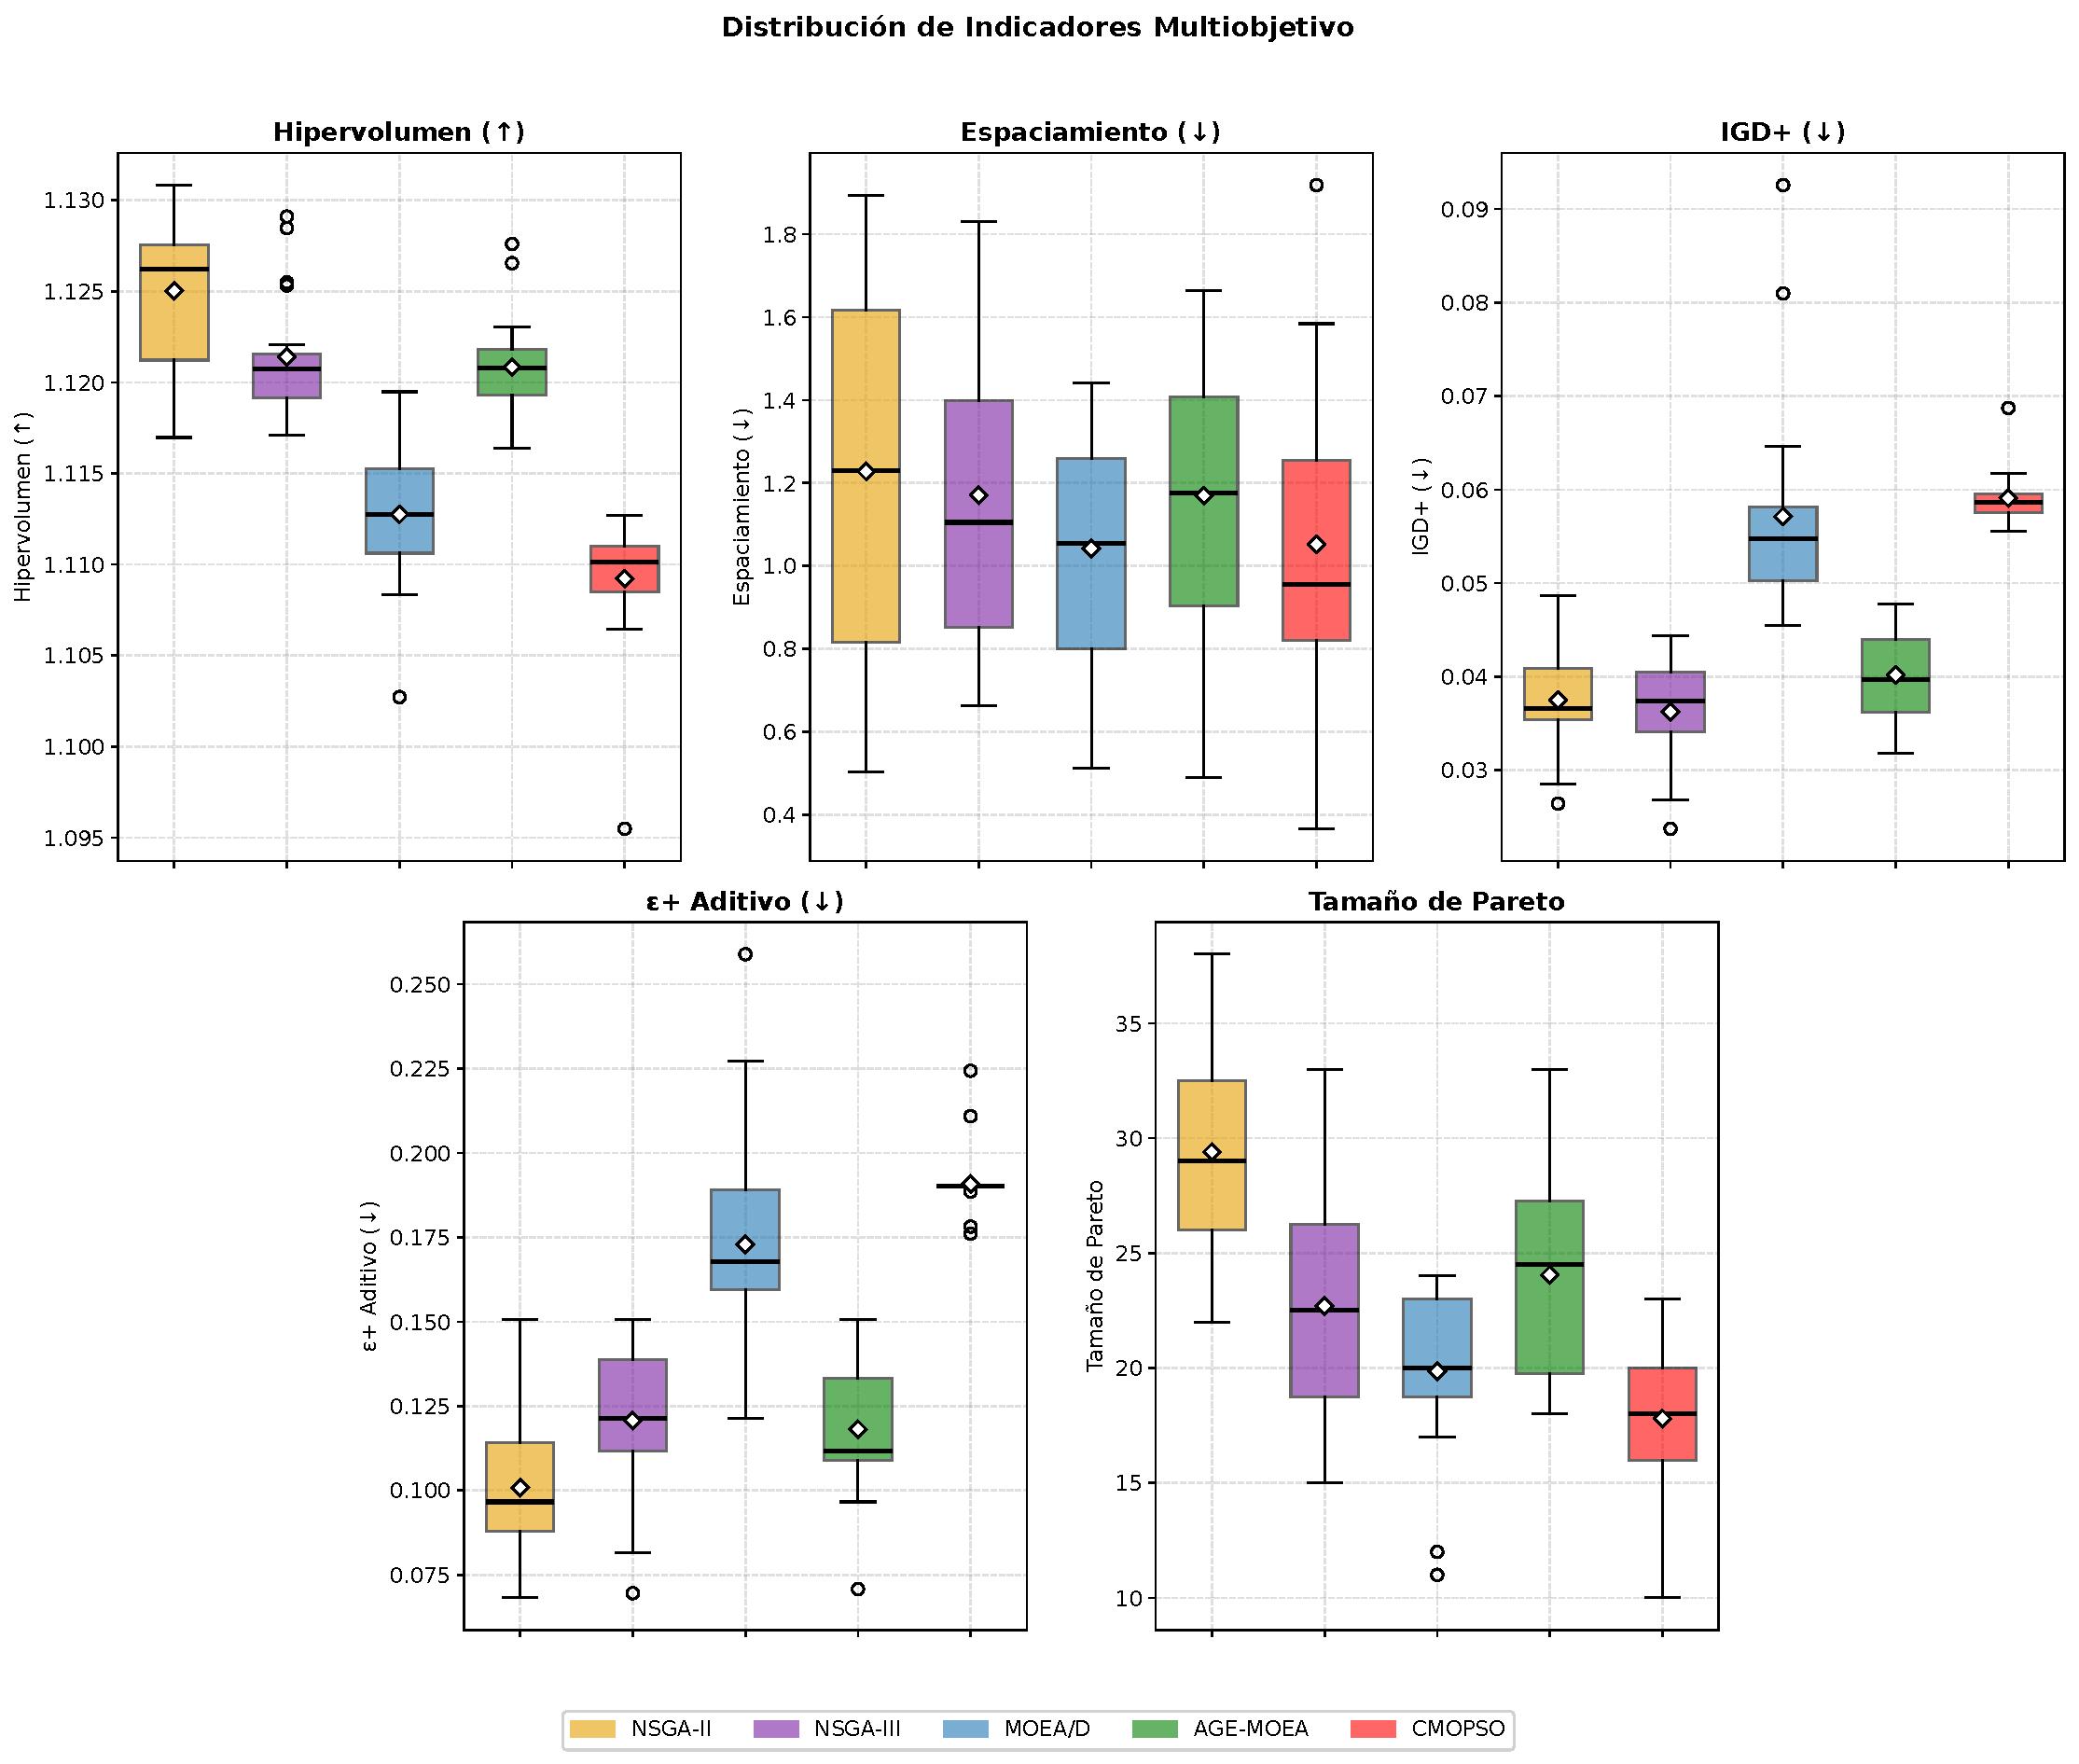
\includegraphics[width=\textwidth]{Figures/metaheuristicas/comparacion/boxplots_mo_popfinal.pdf}
    \caption{Distribución de los indicadores multiobjetivo de cada algoritmo sobre las veinte ejecuciones independientes.}
    \label{fig:boxplots_mo}
\end{figure}

La Figura~\ref{fig:boxplots_mo} ilustra la distribución de los indicadores multiobjetivo de la Tabla~\ref{tab:comparison_multiobjective} mediante diagramas de caja. \acrshort{nsga2} obtiene las medianas más favorables en hipervolumen ($\approx 1.126$), $\text{IGD}^+$ y $\epsilon^+$, junto con el mayor número de soluciones no dominadas (mediana de $29$). \acrshort{agemoea} y \acrshort{nsga3} muestran distribuciones similares entre sí en todas las métricas, manteniendo una buena aproximación y cobertura del frente de referencia.

Por su parte, \acrshort{moead} y \acrshort{cmopso} presentan medianas menores de espaciamiento ($1.05$ y $0.95$) debido a que sus soluciones se concentran en el tramo de alto \gls{qed}. Sin embargo, al no explorar la rama de bajo SA, registran valores peores en $\text{IGD}^+$ y $\epsilon^+$, ya que dejar ese sector sin cubrir aumenta la distancia respecto al frente de referencia. Además, al enfocarse en una zona más acotada, obtienen menos soluciones no dominadas (medianas de $20$ y $18$ moléculas, respectivamente).

\begin{figure}[H]
    \centering
    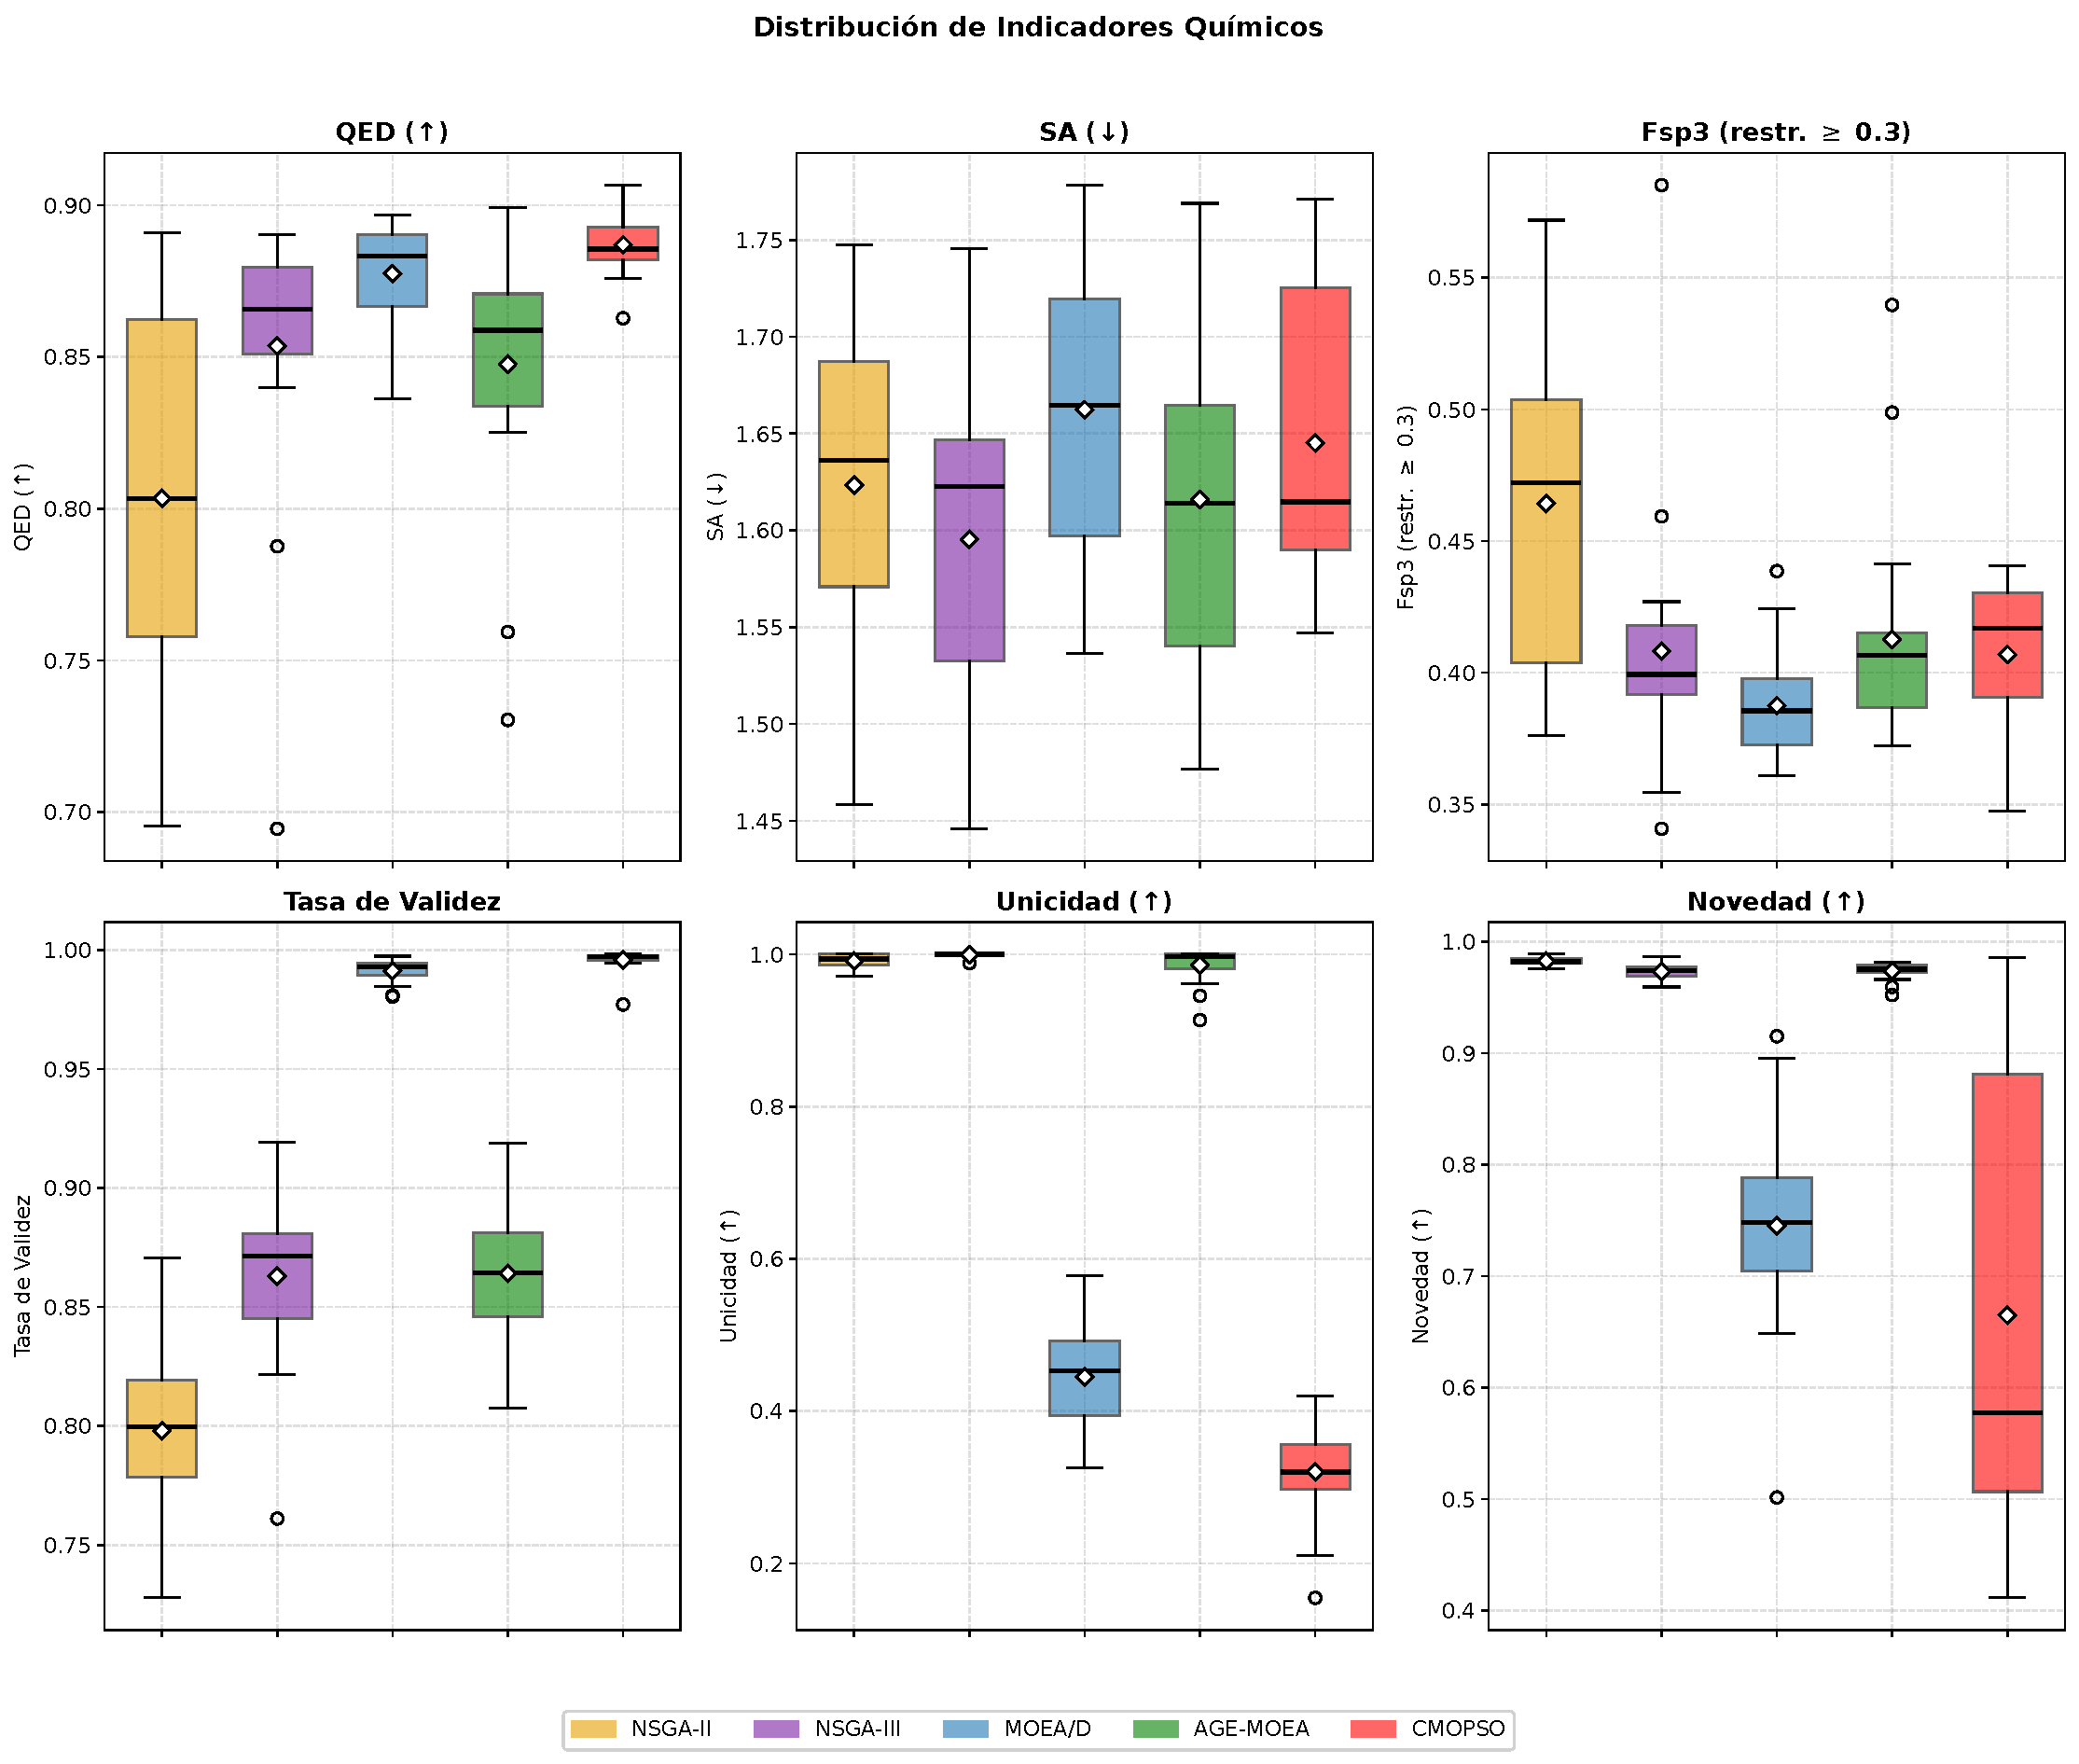
\includegraphics[width=\textwidth]{Figures/metaheuristicas/comparacion/boxplots_chemical_popfinal.pdf}
    \caption{Distribución de las propiedades químicas del frente de Pareto obtenido por cada algoritmo.}
    \label{fig:boxplots_chemical}
\end{figure}

La Figura~\ref{fig:boxplots_chemical} ilustra mediante diagramas de caja las distribuciones de la Tabla~\ref{tab:comparison_chemical} a lo largo de las veinte ejecuciones. En ella, \gls{qed}, SA y $F_{\text{sp3}}$ se evalúan sobre las moléculas del frente no dominado, mientras que la validez, unicidad y novedad describen la generación global de cada ejecución.

En los objetivos, \acrshort{cmopso} y \acrshort{moead} concentran sus resultados de \gls{qed} en torno a $0.88$, mientras que \acrshort{nsga2} presenta mayor dispersión con valores entre $0.70$ y $0.88$, reflejando su cobertura sobre el frente. En accesibilidad sintética, todos los métodos obtienen valores favorables con medianas entre $1.60$ y $1.66$. Respecto a la restricción $F_{\text{sp3}} \ge 0.30$, todos los algoritmos la cumplen, alcanzando \acrshort{nsga2} los valores más altos cerca de $0.47$.

En las métricas de generación, \acrshort{moead} y \acrshort{cmopso} alcanzan una validez próxima al $99\%$, pero su unicidad desciende a medianas de $0.45$ y $0.32$, y su novedad resulta menor y dispersa en \acrshort{cmopso}. En contraste, \acrshort{nsga2}, \acrshort{nsga3} y \acrshort{agemoea} mantienen unicidad y novedad cercanas a $1.0$ y $0.98$, con una validez situada entre el $80\%$ y el $86\%$.

\subsection{Convergencia, Cobertura y Diversidad de las Soluciones}
\label{subsec:convergencia_cobertura_diversidad}

\begin{figure}[H]
    \centering
    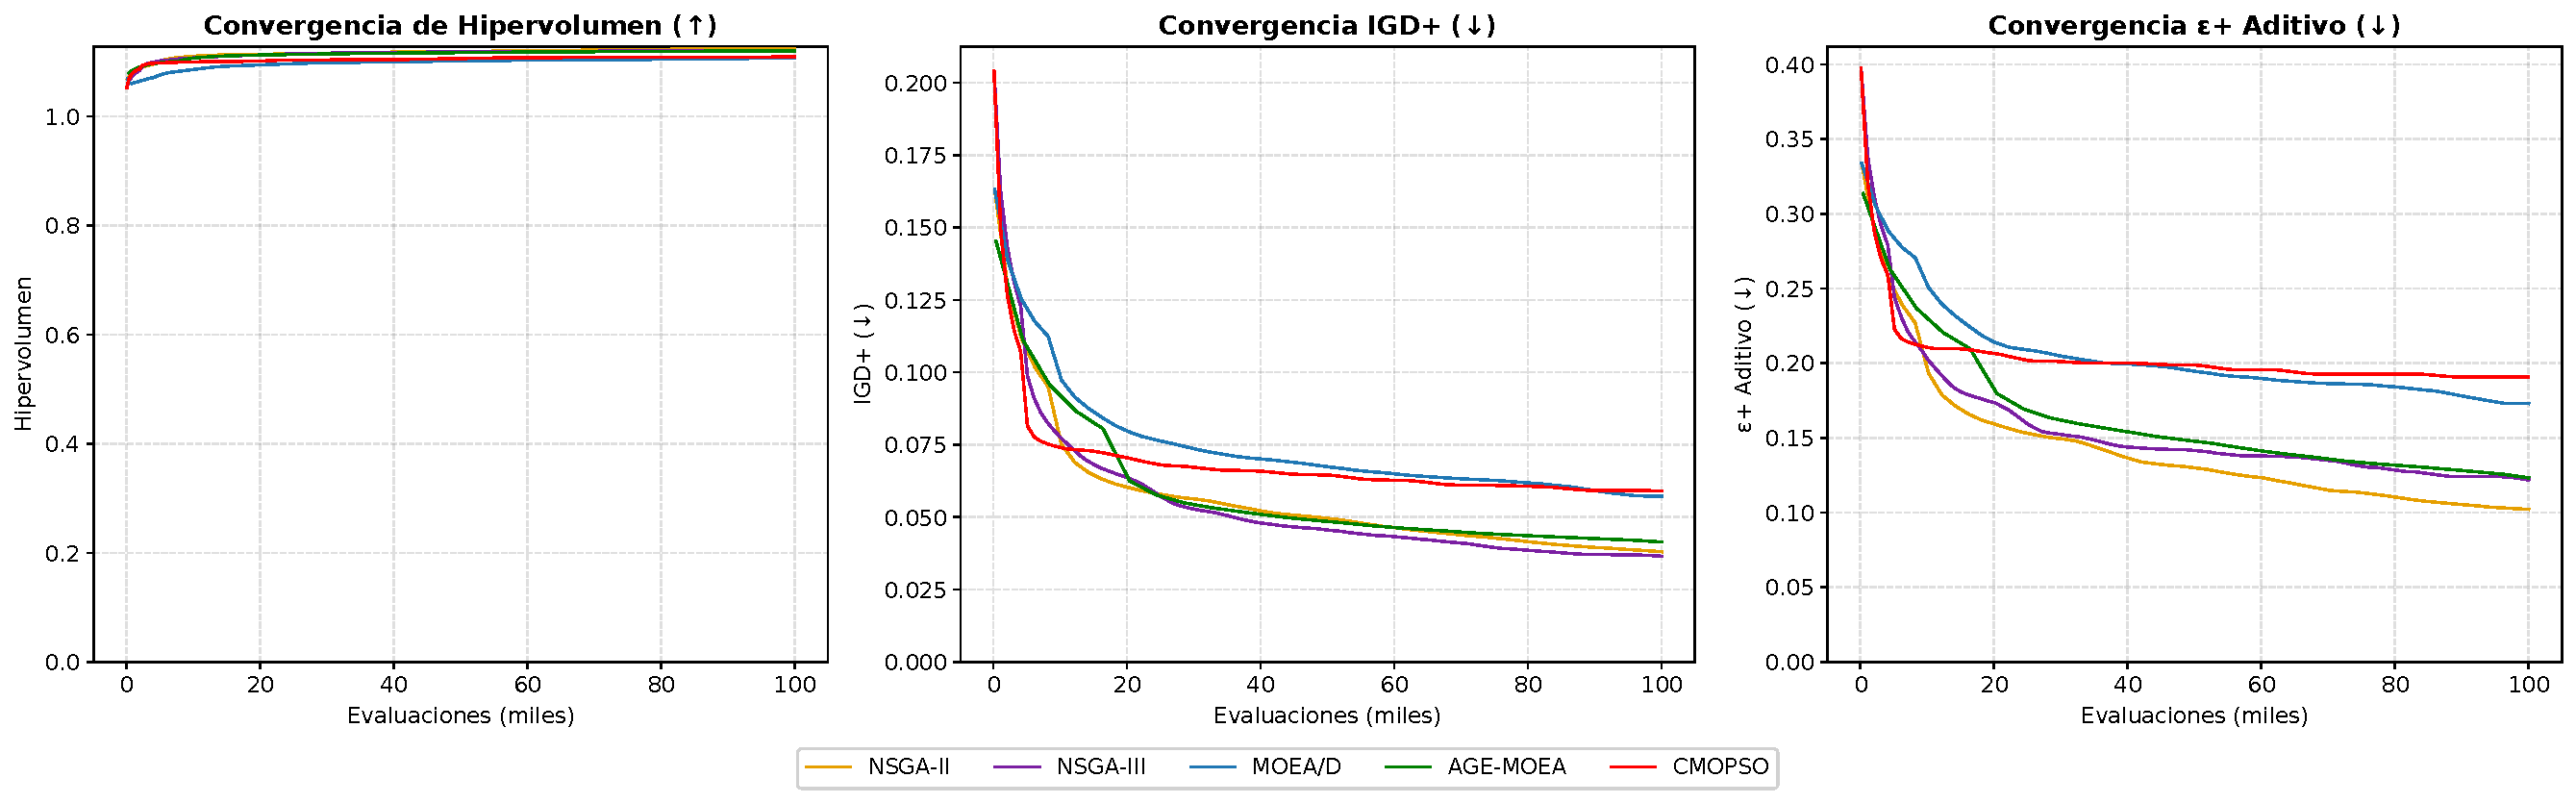
\includegraphics[width=\textwidth]{Figures/metaheuristicas/comparacion/convergence_mo_evals_popfinal.pdf}
    \caption{Convergencia de los indicadores multiobjetivo en función del número de evaluaciones para cada algoritmo, promediada sobre las veinte ejecuciones independientes.}
    \label{fig:convergence_mo}
\end{figure}

La Figura~\ref{fig:convergence_mo} presenta la convergencia de los indicadores multiobjetivo en función del número de evaluaciones, promediada sobre las veinte ejecuciones independientes. Estas curvas muestran el progreso del frente no dominado a lo largo del presupuesto y convergen hacia los valores reportados en la Tabla~\ref{tab:comparison_multiobjective}.

En hipervolumen, todos los algoritmos experimentan un avance rápido durante las primeras $20{,}000$ evaluaciones, superando valores de $1.10$, para luego ingresar en una fase de refinamiento gradual. \acrshort{nsga2} consolida la cota más alta a lo largo de todo el proceso ($1.125$), seguido por \acrshort{nsga3} ($1.121$) y \acrshort{agemoea} ($1.121$), mientras que \acrshort{cmopso} ($1.109$) y \acrshort{moead} ($1.107$) se estabilizan en niveles inferiores desde etapas tempranas, ratificando la jerarquía obtenida en los tests estadísticos.

En $\text{IGD}^+$ y $\epsilon^+$, las trayectorias evidencian diferencias en la dinámica de exploración. \acrshort{cmopso} desciende durante las primeras $10{,}000$ evaluaciones al concentrar sus partículas en la zona de alto \gls{qed}, alcanzando $\text{IGD}^+ \approx 0.073$ y $\epsilon^+ \approx 0.210$. Sin embargo, su progreso se detiene a partir de las $40{,}000$ evaluaciones y finaliza con los valores más desfavorables ($0.059$ y $0.191$). \acrshort{moead} muestra un descenso más progresivo pero igualmente limitado, concluyendo en $0.057$ y $0.173$. Este comportamiento confirma que ambos métodos dejan sectores periféricos del frente de referencia sin cubrir.

Por el contrario, los algoritmos \acrshort{nsga2}, \acrshort{nsga3} y \acrshort{agemoea} logran una mejora sostenida a lo largo de todo el presupuesto. \acrshort{nsga2} registra el menor $\epsilon^+$ desde las $10{,}000$ evaluaciones y concluye en $0.101$, mientras que el menor $\text{IGD}^+$ lo alcanza \acrshort{nsga3} ($0.036$), seguido de \acrshort{nsga2} ($0.038$) y \acrshort{agemoea} ($0.040$). La capacidad de estos algoritmos para extender soluciones hacia el extremo de bajo SA explica que continúen descubriendo nuevas alternativas no dominadas a lo largo de la optimización.

\begin{figure}[H]
    \centering
    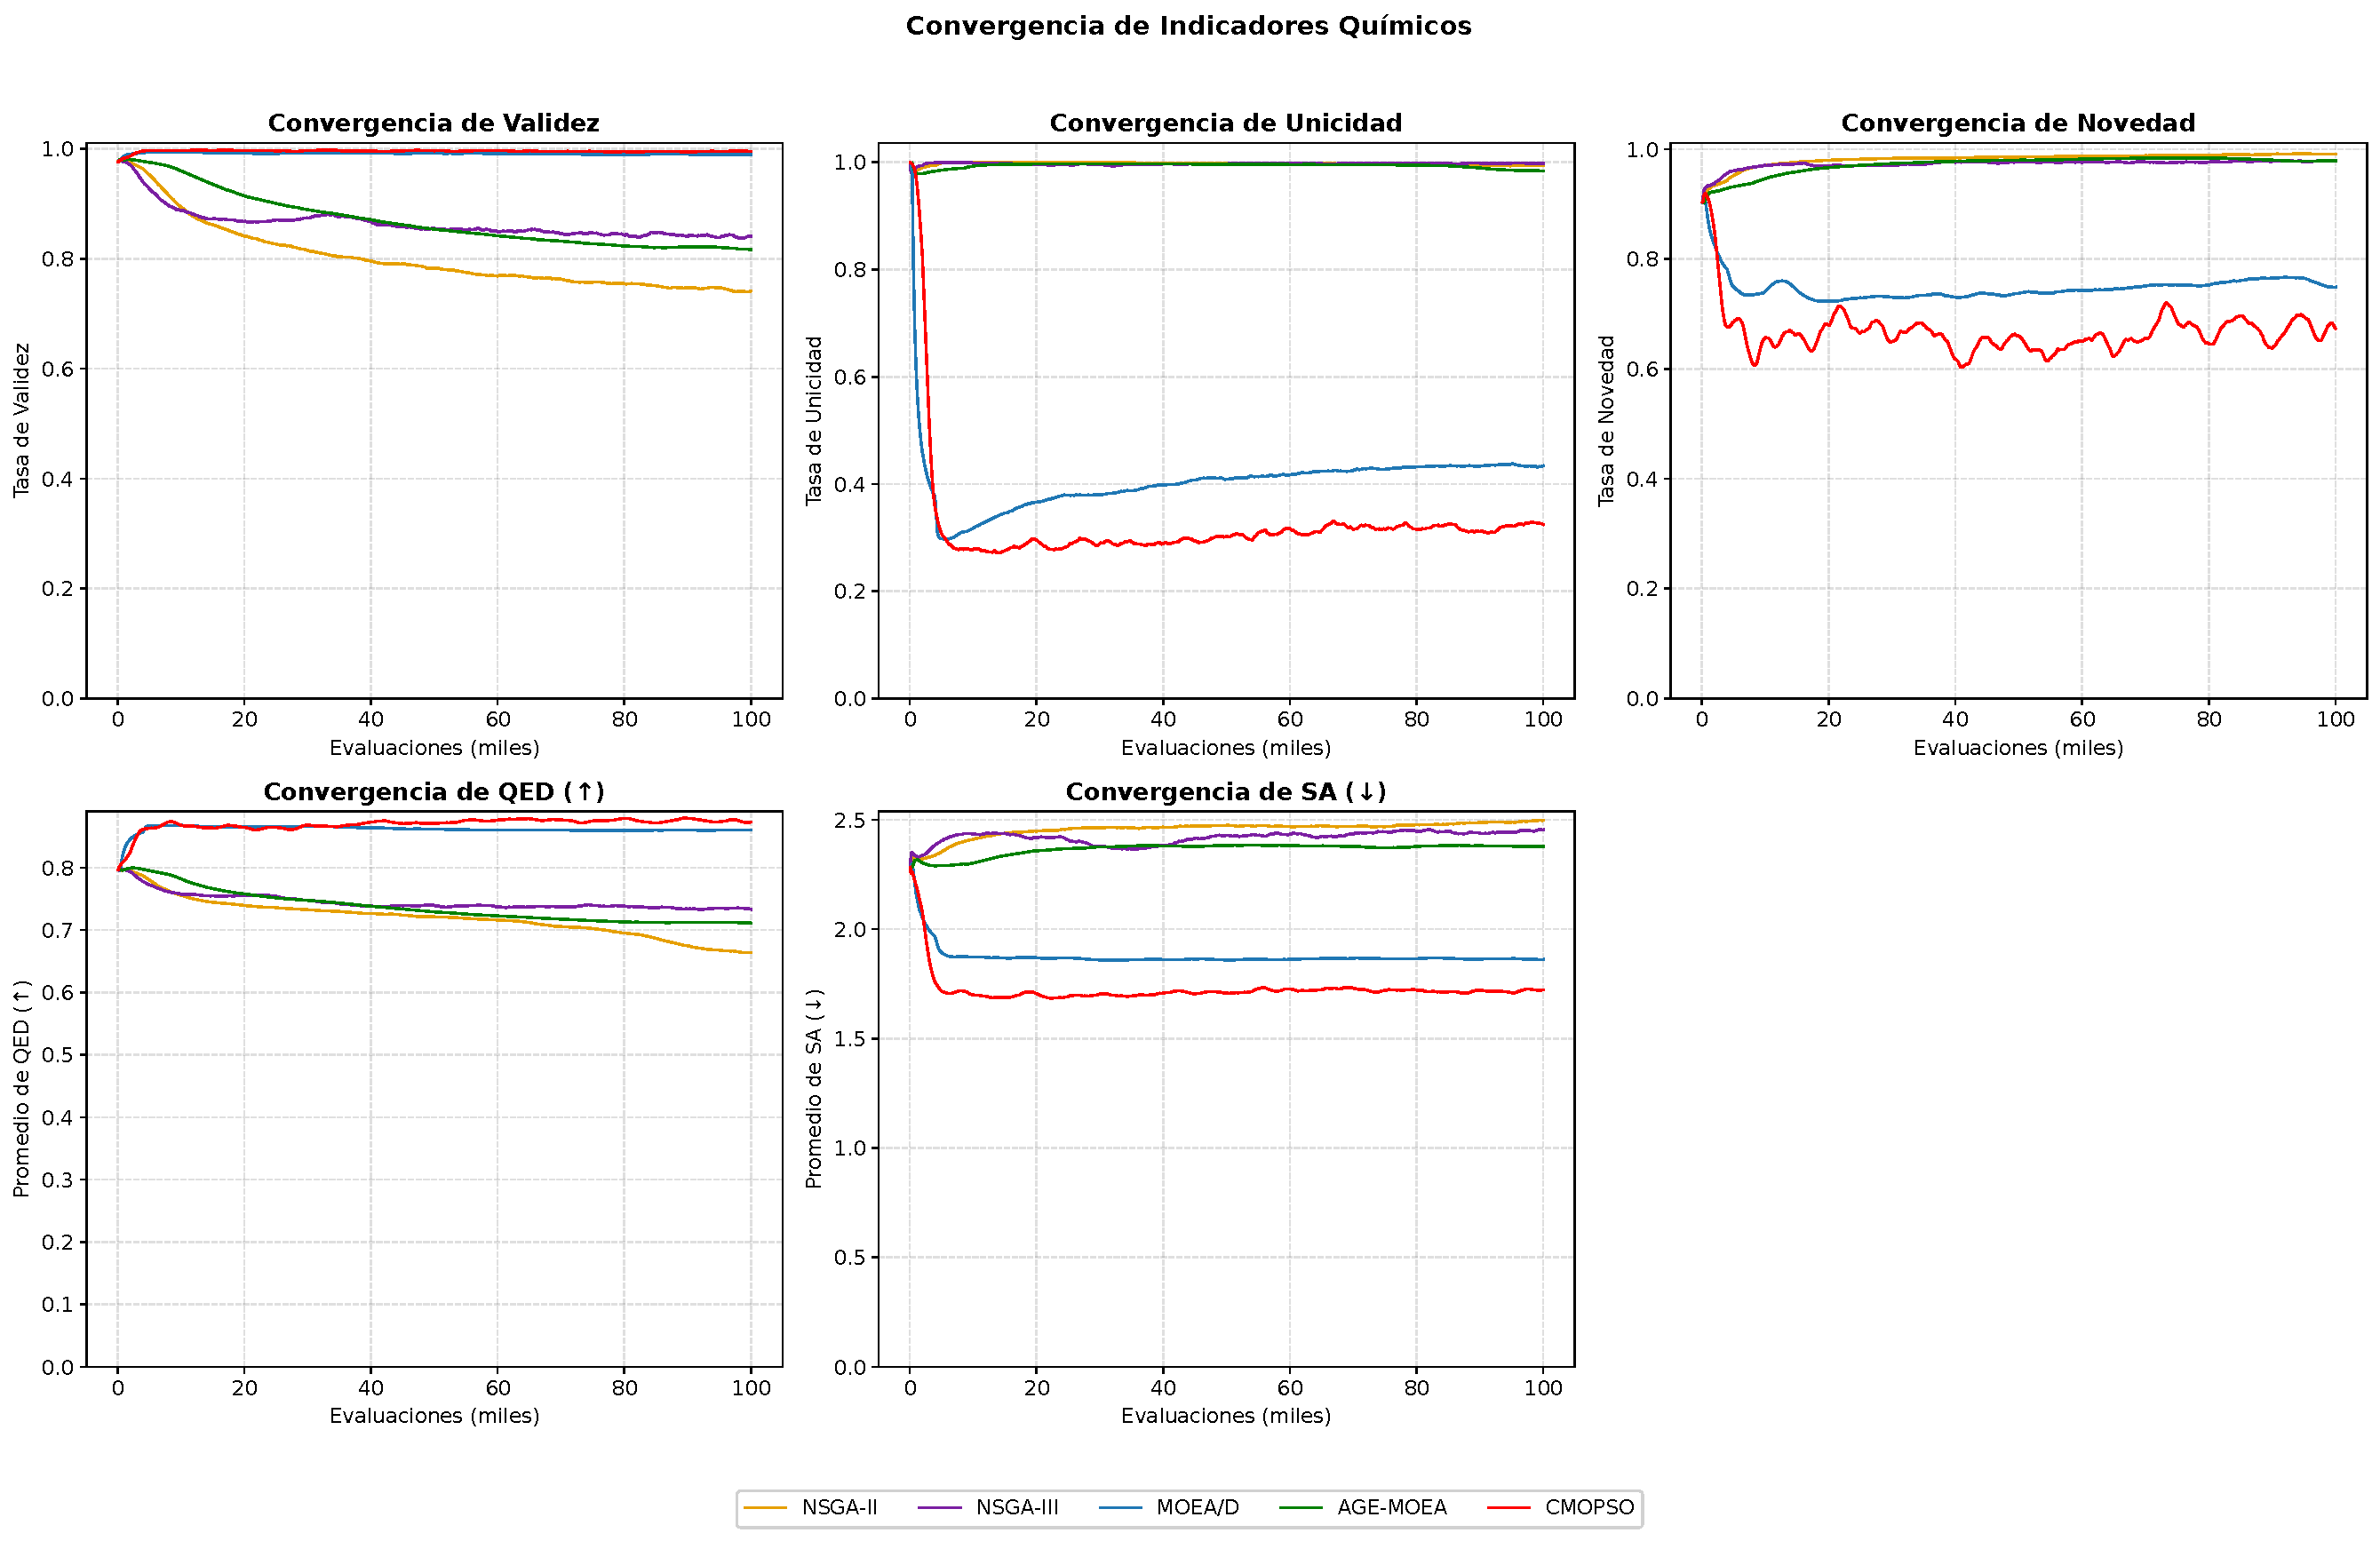
\includegraphics[width=\textwidth]{Figures/metaheuristicas/comparacion/convergence_chemical_evals_popfinal.pdf}
    \caption{Convergencia de los indicadores químicos en función del número de evaluaciones para cada algoritmo, promediada sobre las veinte ejecuciones independientes.}
    \label{fig:convergence_chemical}
\end{figure}

La Figura~\ref{fig:convergence_chemical} muestra la dinámica de las propiedades químicas en la población activa a lo largo de las evaluaciones. \acrshort{moead} y \acrshort{cmopso} sostienen una validez cercana al $99\%$ durante toda la optimización, pero su unicidad desciende durante las primeras $5{,}000$ evaluaciones y se estabiliza entre el $30\%$ y el $44\%$. En cuanto a la novedad frente a los compuestos de entrenamiento, \acrshort{moead} se sitúa en torno al $75\%$ y \acrshort{cmopso} alrededor del $66\%$. Por el contrario, \acrshort{nsga2}, \acrshort{nsga3} y \acrshort{agemoea} conservan una unicidad y novedad próximas al $98\%$ y $100\%$, con una validez que se sitúa entre el $75\%$ y el $84\%$. En el espacio de objetivos de la población activa, \acrshort{cmopso} y \acrshort{moead} concentran sus soluciones en valores promedio de \gls{qed} cercanos a $0.88$ y SA inferior a $1.86$, mientras que los algoritmos genéticos registran un \gls{qed} promedio en torno a $0.66\text{--}0.73$ y un SA superior a $2.37$, reflejando la presencia continua de individuos en diversas regiones del frente.

\subsubsection{Frentes de Pareto}

\begin{figure}[H]
    \centering
    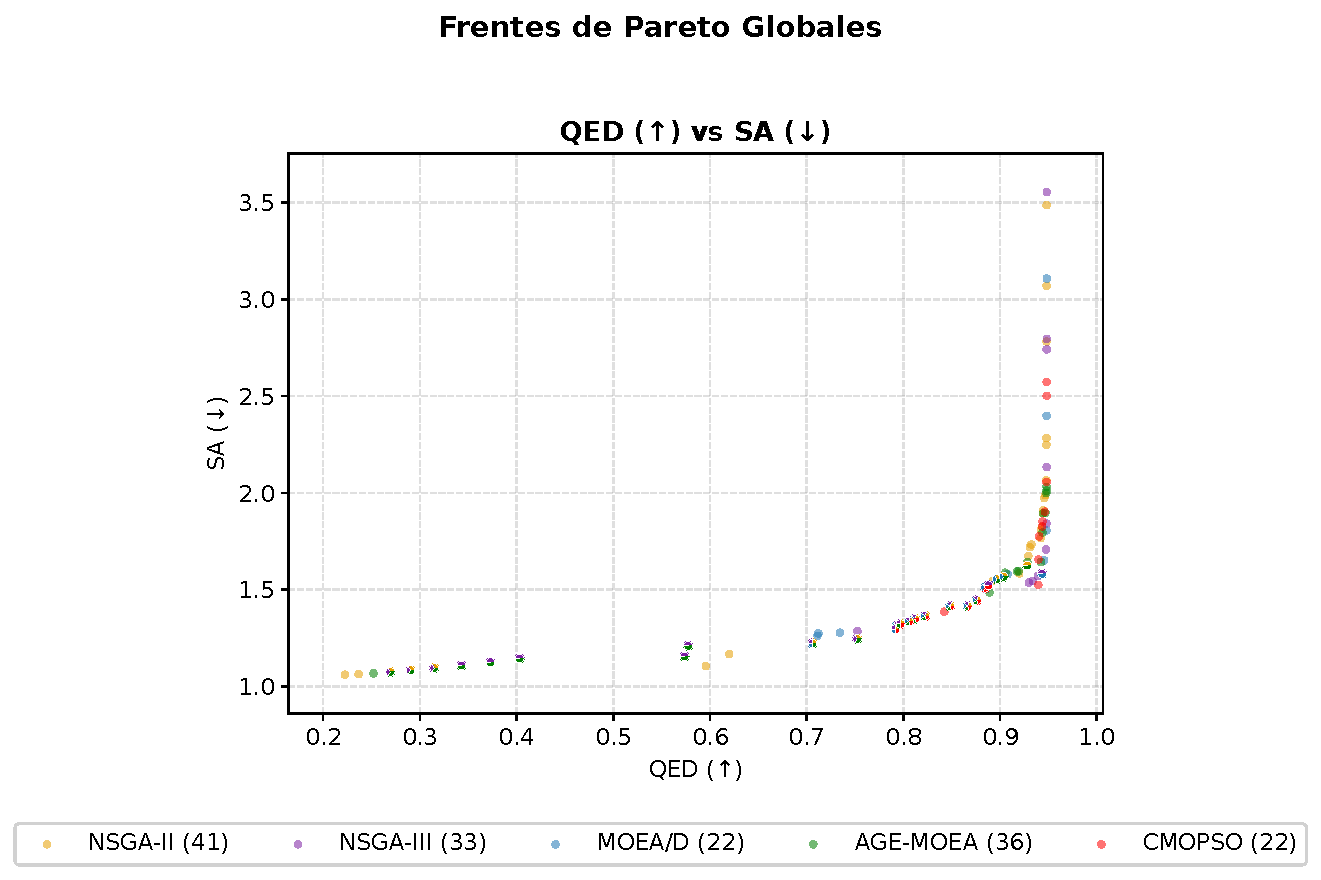
\includegraphics[width=\textwidth]{Figures/metaheuristicas/comparacion/pareto_comparison_popfinal.pdf}
    \caption{Frentes de Pareto superpuestos de las mejores configuraciones de los cinco algoritmos en el espacio QED--SA.}
    \label{fig:pareto_comparison}
\end{figure}

La Figura~\ref{fig:pareto_comparison} muestra los frentes de Pareto acumulados de los cinco algoritmos en el espacio \gls{qed}--SA sobre las veinte ejecuciones. Todos los métodos comparten el frente general, aunque con diferencias en la cantidad y distribución de las soluciones. \acrshort{nsga2} acumula el mayor número de moléculas no dominadas ($41$), seguido por \acrshort{agemoea} ($36$) y \acrshort{nsga3} ($33$), mientras que \acrshort{cmopso} y \acrshort{moead} obtienen solo $22$ cada uno, en línea con el tamaño de frente reportado en la Tabla~\ref{tab:comparison_multiobjective}.

En la región de bajo SA, los algoritmos genéticos son los únicos que encuentran soluciones, alcanzando \acrshort{nsga2} los compuestos de menor SA ($\approx 1.06$). En cambio, \acrshort{cmopso} y \acrshort{moead} no exploran esta zona y limitan su búsqueda a valores de \gls{qed} superiores a $0.70$. Hacia el centro del frente, los cinco métodos coinciden y comparten soluciones con un equilibrio adecuado entre ambas propiedades.

En el extremo de alto \gls{qed}, el frente forma una rama vertical donde los valores se saturan cerca de $0.948$. En este tramo, mejoras mínimas en \gls{qed} exigen estructuras más complejas y elevan el SA por encima de $3.0$, donde \acrshort{nsga2} y \acrshort{nsga3} alcanzan las soluciones más altas. Esta distribución explica por qué \acrshort{cmopso} y \acrshort{moead} obtienen un \gls{qed} promedio superior en la Tabla~\ref{tab:comparison_chemical}, ya que concentran sus soluciones en la derecha, mientras que los algoritmos genéticos reducen su promedio al incluir también alternativas de fácil síntesis.



\subsection{Análisis del Frente no Dominado Conjunto y Moléculas Representativas}
\label{subsec:frente_conjunto_global}

Para evaluar la capacidad exploratoria conjunta y caracterizar el espacio químico accesible, se combinan las soluciones obtenidas por las ramas de cruce PCX y SBX en los cuatro algoritmos genéticos (empleando en cada caso el operador de mutación con mejor desempeño en la comparación estadística), junto con \acrshort{cmopso}, a lo largo de las veinte ejecuciones independientes. Tras deduplicar por estructura química (\gls{smiles}), se recalcula la no dominancia global, conformando un frente no dominado conjunto de 32 moléculas únicas.

\subsubsection{Contribución al Frente Conjunto Global}

La Tabla~\ref{tab:contribucion_pool} presenta la contribución de cada algoritmo y combinación de operadores al frente no dominado conjunto global, indicando el número de moléculas aportadas, las exclusivas, el porcentaje sobre el total y los promedios de los objetivos en las soluciones aportadas.

\begin{table}[H]
\centering
\caption{Contribución de cada algoritmo y combinación de operadores al frente no dominado conjunto global (32 soluciones).}
\label{tab:contribucion_pool}
\begin{tabular}{llrrrrrr}
\toprule
Configuración & Operadores & Aporta & Exclusivas & \% & QED $\uparrow$ & SA $\downarrow$ & $F_{\text{sp3}}$ \\
\midrule
\multirow{2}{*}{\acrshort{nsga2}} & pcx\_pm & 15 & 4 & 46.9 & 0.598 & 1.220 & 0.570 \\
 & sbx\_gauss & 16 & 6 & 50.0 & 0.874 & 1.590 & 0.338 \\
\midrule
\multirow{2}{*}{\acrshort{nsga3}} & pcx\_pm & 15 & 2 & 46.9 & 0.726 & 1.470 & 0.475 \\
 & sbx\_pm & 9 & 1 & 28.1 & 0.829 & 1.480 & 0.347 \\
\midrule
\multirow{2}{*}{\acrshort{moead}} & pcx\_pm & 9 & 0 & 28.1 & 0.841 & 1.410 & 0.343 \\
 & sbx\_pm & 6 & 0 & 18.8 & 0.828 & 1.370 & 0.359 \\
\midrule
\multirow{2}{*}{\acrshort{agemoea}} & pcx\_pm & 11 & 1 & 34.4 & 0.615 & 1.240 & 0.587 \\
 & sbx\_pm & 7 & 0 & 21.9 & 0.811 & 1.350 & 0.350 \\
\midrule
\acrshort{cmopso} & - & 10 & 3 & 31.2 & 0.865 & 1.620 & 0.360 \\
\bottomrule
\end{tabular}
\end{table}

En la Tabla~\ref{tab:contribucion_pool} se observa que \acrshort{nsga2} lidera la contribución al frente global, aportando el $50.0\%$ de las soluciones mediante sbx\_gauss ($16$ moléculas, $6$ exclusivas) y el $46.9\%$ mediante pcx\_pm ($15$ moléculas, $4$ exclusivas). \acrshort{nsga3} y \acrshort{agemoea} también realizan aportes importantes, mientras que \acrshort{cmopso} suma $10$ soluciones ($3$ de ellas exclusivas, representando el $31.2\%$). Por su parte, las soluciones de \acrshort{moead} resultan compartidas con las aportadas por los demás algoritmos.

Nuevamente se comprueba la complementariedad entre familias de operadores: las combinaciones con PCX aportan las moléculas con mayor grado de saturación ($F_{\text{sp3}}$ medio de $0.48\text{--}0.59$) y menor dificultad sintética (SA $\approx 1.220\text{--}1.470$, aunque con menor \gls{qed}), mientras que las variantes con SBX y \acrshort{cmopso} consolidan la zona de alto \gls{qed} ($> 0.81\text{--}0.87$) con valores de $F_{\text{sp3}}$ en torno a $0.34\text{--}0.36$.

\begin{figure}[H]
    \centering
    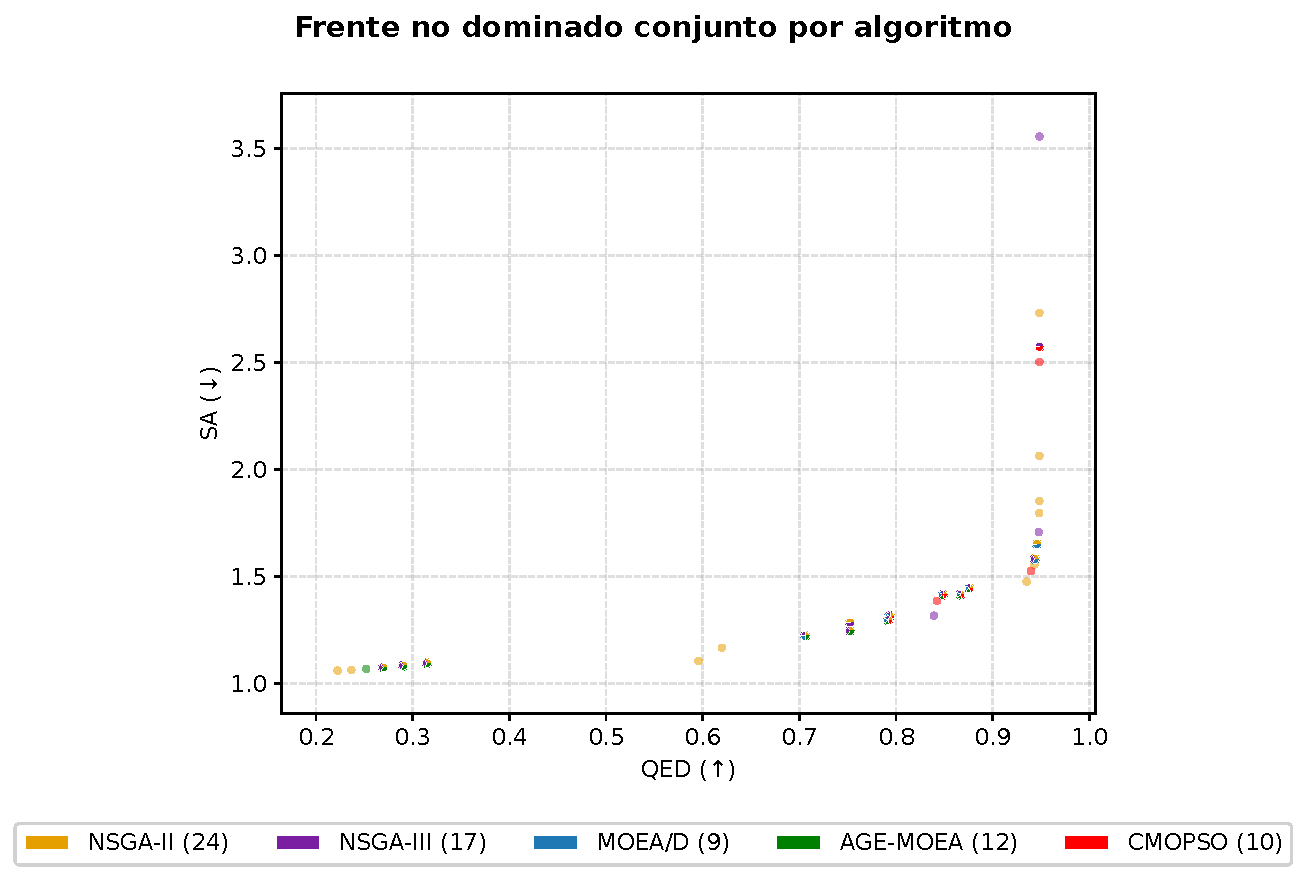
\includegraphics[width=\textwidth]{Figures/metaheuristicas/frente_conjunto/frente_conjunto_poppool.pdf}
    \caption{Frente no dominado conjunto global (32 soluciones) en el espacio QED--SA, coloreado según el algoritmo aportante.}
    \label{fig:frente_conjunto_poppool}
\end{figure}

La Figura~\ref{fig:frente_conjunto_poppool} presenta la distribución de las 32 soluciones del frente no dominado conjunto en el espacio \gls{qed}--SA. Los círculos de un solo color representan aportes exclusivos de un algoritmo, mientras que las divisiones multicolores indican moléculas descubiertas por más de un método.

\acrshort{nsga2} muestra la mayor cobertura al participar en 24 de las 32 soluciones y aportar 10 de forma exclusiva, abarcando los compuestos de menor SA en solitario y compartiendo la zona intermedia de esa cola con \acrshort{agemoea} y \acrshort{nsga3}. En el centro del frente, la presencia de puntos multicolores refleja convergencia hacia las mismas estructuras de compromiso, mientras que en la rama vertical de alto \gls{qed} destacan aportes de \acrshort{cmopso}, \acrshort{nsga2} y la molécula de mayor SA descubierta por \acrshort{nsga3}.

\subsubsection{Moléculas Representativas}

Para analizar la calidad de las moléculas generadas y comparar cómo explora cada metaheurística las distintas regiones del frente de Pareto, se seleccionan tres soluciones representativas por algoritmo: la de menor dificultad sintética (menor SA), la de mayor valor de \gls{qed}, y la del extremo de mayor SA dentro del frente no dominado. La Tabla~\ref{tab:moleculas_representativas} y la Figura~\ref{fig:moleculas_representativas} presentan sus propiedades fisicoquímicas y estructuras 2D. El catálogo completo de las cinco moléculas de mayor \gls{qed} por algoritmo se encuentra disponible en el Apéndice~\ref{sec:apendice_moleculas_top_qed} (Tabla~\ref{tab:moleculas_representativas_completo}).

\begin{table}[H]
\centering
\caption{Moléculas representativas de cada algoritmo en tres puntos del frente de Pareto: extremo de menor SA, mayor QED y extremo de mayor SA.}
\label{tab:moleculas_representativas}
\resizebox{\textwidth}{!}{%
\begin{tabular}{llcccl}
\toprule
\textbf{Algoritmo} & \textbf{Punto del Frente} & \textbf{QED} $\uparrow$ & \textbf{SA} $\downarrow$ & \textbf{$F_{\text{sp3}}$} & \textbf{SMILES} \\
\midrule
\multirow{3}{*}{\acrshort{nsga2}}
 & Extremo de menor SA & 0.223 & 1.060 & 1.000 & \texttt{CCCCCCCCCCCCCCCCCCCCC} \\
 & Mayor QED & 0.948 & 1.800 & 0.333 & \texttt{Cc1ccc(NC(=O)N2CCN(Cc3ccccn3)CC2)cc1} \\
 & Extremo de mayor SA & 0.948 & 2.730 & 0.333 & \texttt{Cn1cc(NC(=O)C2CCCO2)c(-c2ccccc2Cl)n1} \\
\midrule
\multirow{3}{*}{\acrshort{nsga3}}
 & Extremo de menor SA & 0.270 & 1.070 & 1.000 & \texttt{CCCCCCCCCCCCCCCCCC} \\
 & Mayor QED & 0.948 & 1.710 & 0.316 & \texttt{Cc1cc(C(=O)N2CCN(Cc3ccccc3)CC2)ccc1O} \\
 & Extremo de mayor SA & 0.948 & 3.550 & 0.312 & \texttt{Cc1cc(CO)c(Cl)c(-c2cccn2C2COCC2=O)c1} \\
\midrule
\multirow{3}{*}{\acrshort{moead}}
 & Extremo de menor SA & 0.706 & 1.220 & 0.300 & \texttt{O=C(Nc1ccccc1)C1CC1} \\
 & Mayor QED & 0.948 & 1.810 & 0.333 & \texttt{Cc1ccc(CN2CCN(C(=O)Nc3cccnc3)CC2)cc1} \\
 & Extremo de mayor SA & 0.948 & 3.110 & 0.333 & \texttt{Cc1nc(C(O)c2ccccc2Cl)n(CC(F)(F)F)n1} \\
\midrule
\multirow{3}{*}{\acrshort{agemoea}}
 & Extremo de menor SA & 0.252 & 1.070 & 1.000 & \texttt{CCCCCCCCCCCCCCCCCCC} \\
 & Mayor QED & 0.948 & 1.810 & 0.333 & \texttt{Cc1ccc(NC(=O)N2CCN(Cc3ccccc3)CC2)cn1} \\
 & Extremo de mayor SA & 0.948 & 2.030 & 0.375 & \texttt{O=C(c1csc(-c2cccc(CO)c2)n1)N1CCCCC1} \\
\midrule
\multirow{3}{*}{\acrshort{cmopso}}
 & Extremo de menor SA & 0.792 & 1.300 & 0.364 & \texttt{CCCNC(=O)c1ccc(OC)cc1} \\
 & Mayor QED & 0.948 & 2.060 & 0.333 & \texttt{O=C(NC1CCN(c2nccs2)CC1)c1ccccc1F} \\
 & Extremo de mayor SA & 0.948 & 2.570 & 0.333 & \texttt{O=C(NC1(c2nccs2)CCOCC1)c1ccccc1F} \\
\bottomrule
\end{tabular}%
}
\end{table}

\begin{figure}[H]
    \centering
    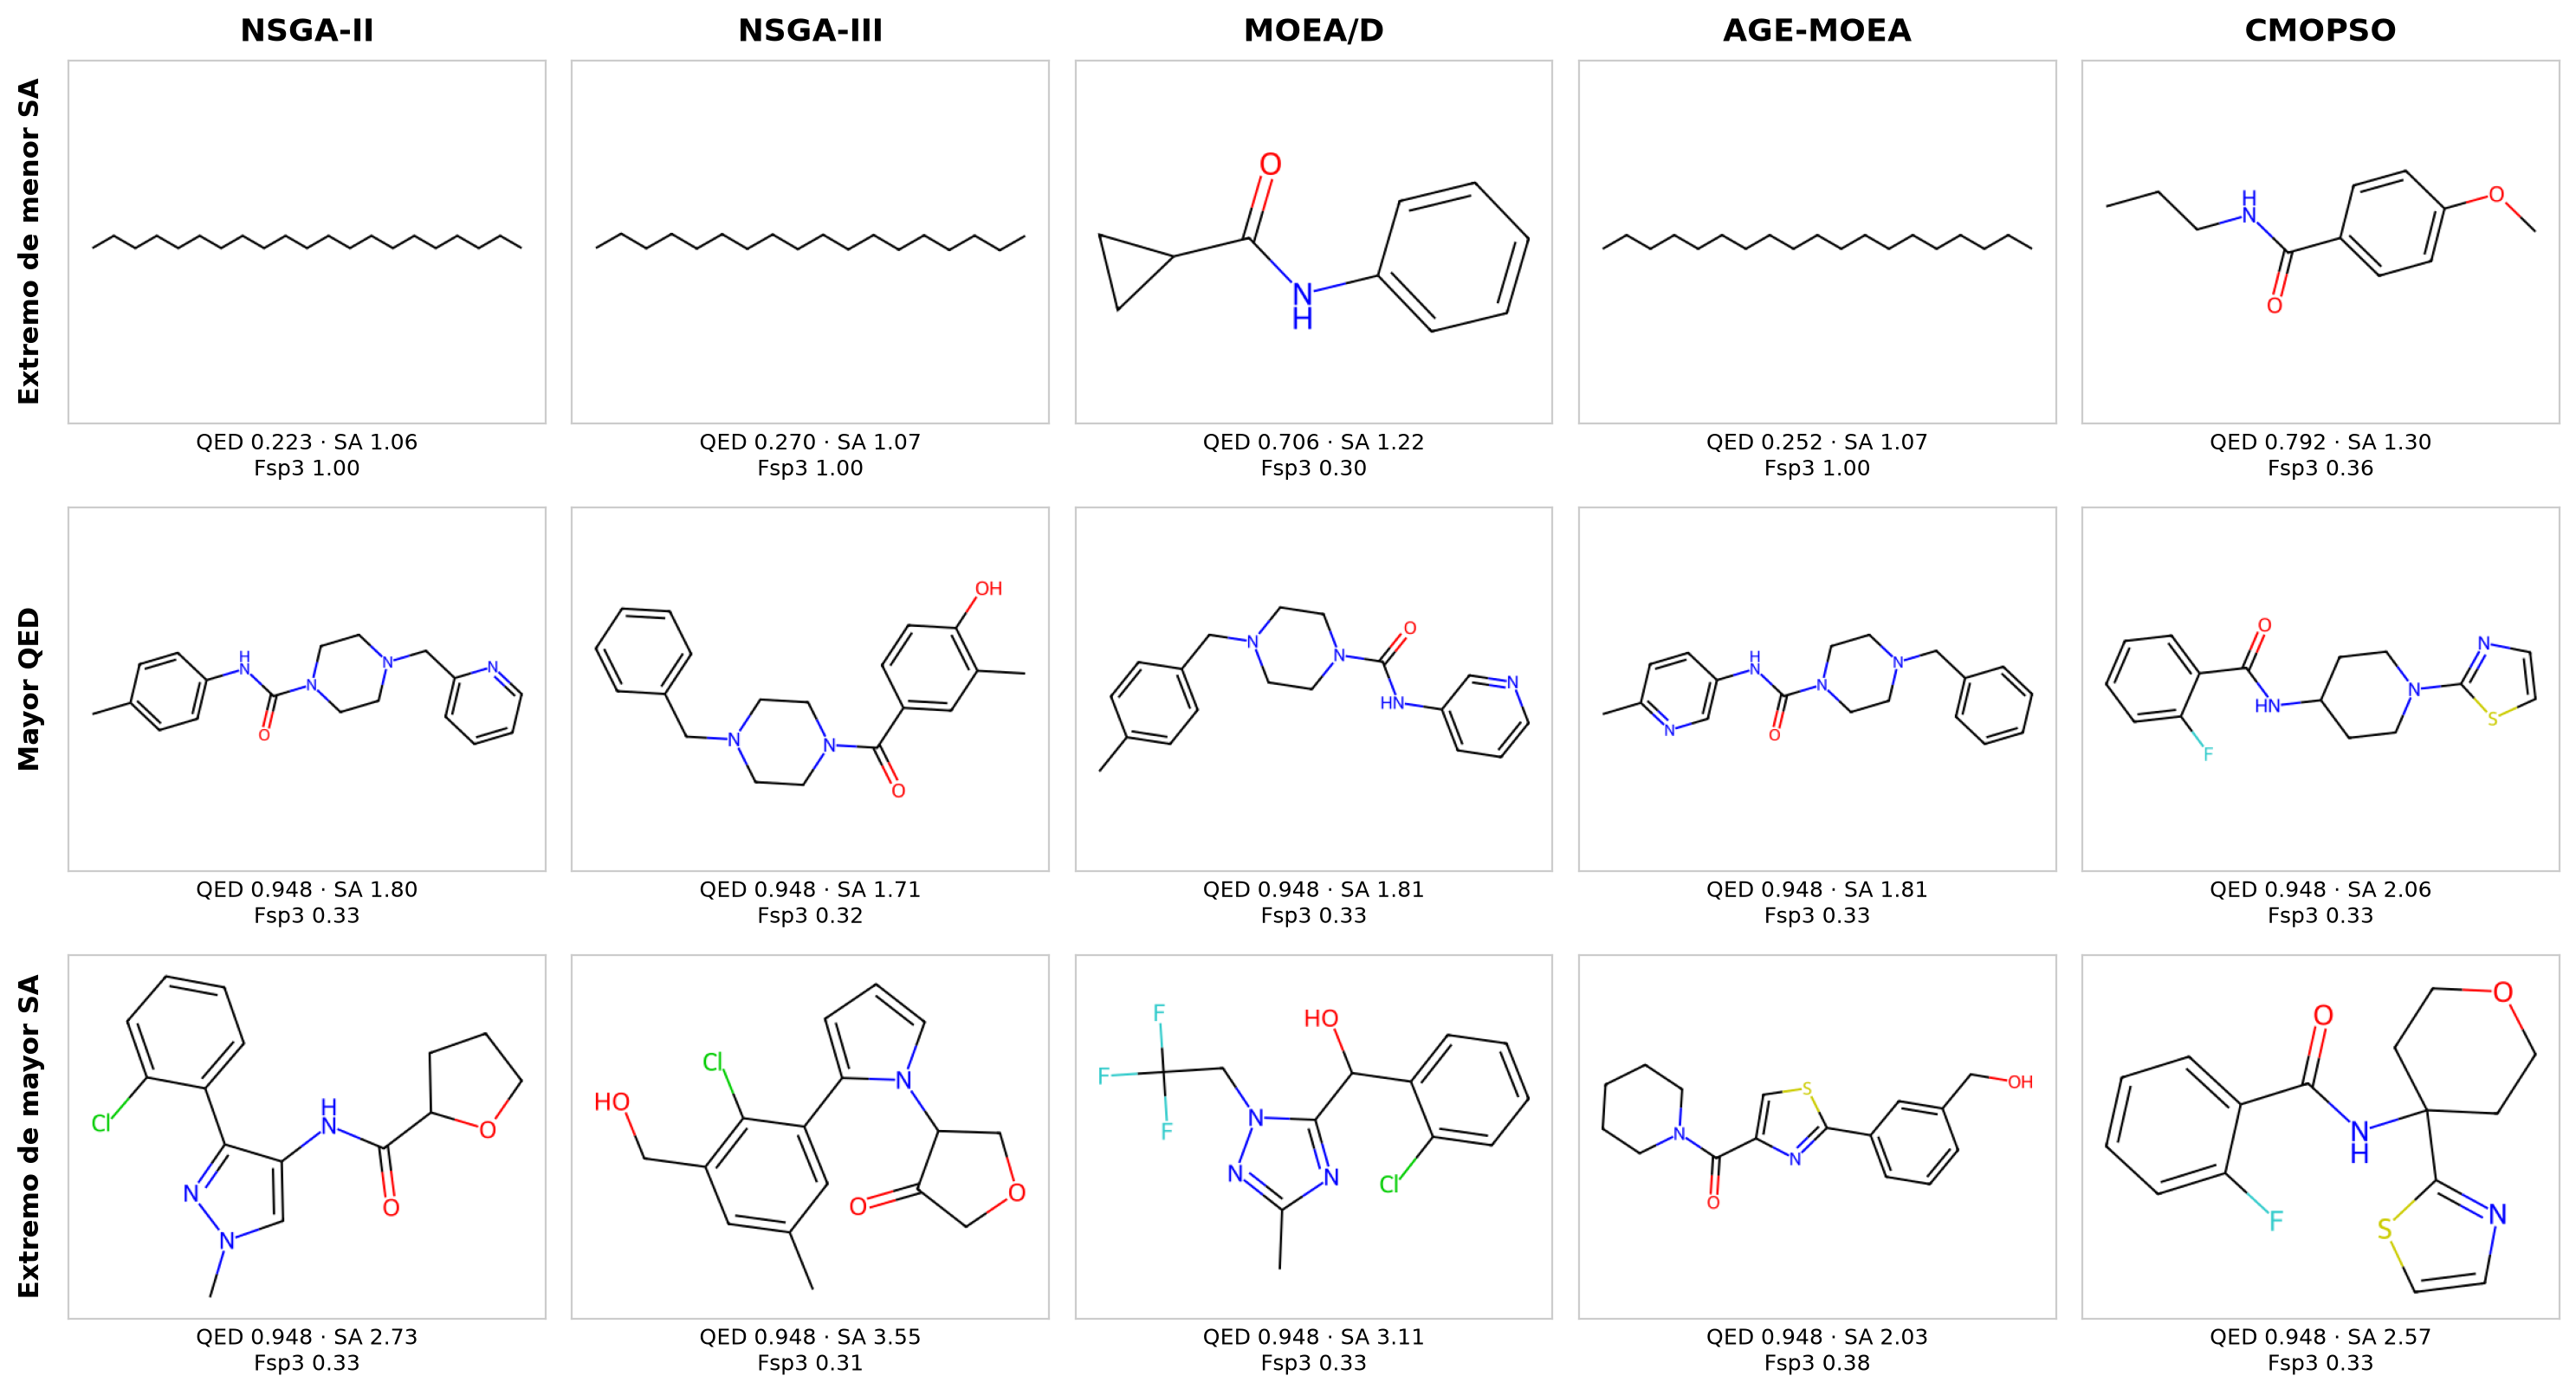
\includegraphics[width=0.95\textwidth]{Figures/metaheuristicas/frente_conjunto/moleculas_representativas.png}
    \caption{Estructuras 2D de las moléculas representativas de cada algoritmo en tres puntos del frente de Pareto: extremo de menor SA, mayor QED y extremo de mayor SA.}
    \label{fig:moleculas_representativas}
\end{figure}

La Tabla~\ref{tab:moleculas_representativas} y la Figura~\ref{fig:moleculas_representativas} muestran las moléculas generadas a lo largo del frente de Pareto. En la zona de menor SA, \acrshort{nsga2}, \acrshort{nsga3} y \acrshort{agemoea} exploran el extremo del espacio generando cadenas lineales de carbono saturadas con bajo \gls{qed}. Aunque estas cadenas no presentan interés como fármacos, la capacidad de estos algoritmos para explorar los extremos del frente puede resultar útil al incorporar otros objetivos a optimizar. Por el contrario, \acrshort{moead} y \acrshort{cmopso} son más conservadores en esta región y generan moléculas pequeñas con mejor perfil farmacológico.

En la zona de mayor \gls{qed}, todos los métodos convergen alrededor de $0.948$ y producen estructuras similares basadas en anillos aromáticos combinados con piperazina o piperidina. En este punto, \acrshort{nsga3} destaca al obtener la molécula de mayor \gls{qed} con la menor dificultad sintética entre todos los algoritmos. Finalmente, en el extremo de mayor SA, el \gls{qed} se satura mientras el SA aumenta debido a la incorporación de más anillos y sustituyentes. Esto explica por qué el frente de Pareto se vuelve casi vertical en esa zona, ya que agregar más complejidad estructural no produce mejoras en el \gls{qed}.

\subsection{Discusión y Limitaciones}
\label{subsec:discusion_limitaciones_genericos}

La incorporación de $F_{\text{sp3}} \ge 0.30$ como restricción de factibilidad fuerza al modelo a evitar estructuras predominantemente planas, asociadas a baja solubilidad y promiscuidad biológica~\cite{Lovering2009Flatland,Lovering2013Flatland2}. Los resultados muestran que existe complementariedad de los operadores, donde PCX actúa como motor de dispersión y novedad, extendiendo el frente hacia regiones de bajo SA y alta saturación, mientras que SBX y \acrshort{cmopso} concentran la búsqueda en regiones de alto \gls{qed} manteniendo una alta validez química.

En conjunto, estos resultados sugieren que formular la tridimensionalidad como una restricción ayuda a orientar la búsqueda sin sobrecargar la optimización. La combinación de operadores con dinámicas distintas permite explorar diferentes zonas del frente, aportando soluciones factibles que concilian de manera razonable la accesibilidad sintética y las propiedades tipo fármaco evaluadas.

Al no existir un frente de Pareto teórico conocido para este espacio químico, la comparación entre algoritmos esta basada en un frente de referencia empírico construido a partir de las soluciones no dominadas factibles obtenidas.

Por último, las funciones objetivo optimizadas (\gls{qed} y SA) y la restricción impuesta ($F_{\text{sp3}} \ge 0.30$) evalúan propiedades fisicoquímicas generales estimadas computacionalmente, sin medir la afinidad frente a una diana terapéutica particular, aspecto que se aborda en una etapa posterior incorporando acoplamiento molecular.

\section{Generación de Inhibidores de la Proteína \texorpdfstring{\gls{mrp1}}{MRP1}}
\label{sec:res_mrp1}

En esta sección se aborda la optimización multiobjetivo dirigida hacia la diana \gls{mrp1} mediante los algoritmos seleccionados. Se evalúa el desempeño en cuatro objetivos de optimización y la influencia de los operadores de cruce (SBX y PCX), para luego comparar con modelos de referencia y analizar las moléculas candidatas de los frentes de Pareto generados mediante validación conformacional y análisis de características \gls{admet}.

% -----------------------------------------------------------------------------
\subsection{Análisis de Calidad de Generación e Indicadores Multiobjetivo}
\label{subsec:calidad_gen_mrp1}

\subsubsection{Indicadores Multiobjetivo y Propiedades Químicas}
\label{subsubsec:indicadores_multiobjetivo_quimicos}

\begin{table}[H]
\centering
\caption{Comparación de indicadores multiobjetivo por algoritmo y operador de cruce.}
\label{tab:multiobjetivo}
\resizebox{\textwidth}{!}{
\begin{tabular}{lcccccc}
\toprule
Configuración & Hipervolumen $\uparrow$ & Espaciamiento $\downarrow$ & IGD$^+$ $\downarrow$ & $\epsilon^+$ $\downarrow$ & Tamaño de Pareto $\uparrow$ & Tiempo (s) $\downarrow$ \\
\midrule
NSGA-II (SBX) & $0.502 \pm 0.012$ & $0.591 \pm 0.037$ & $0.038 \pm 0.005$ & $\mathbf{0.181 \pm 0.030}$ & $\mathbf{712.8 \pm 109.8}$ & $\text{7.112},8 \pm 264.5$ \\
NSGA-II (PCX) & $0.471 \pm 0.004$ & $0.587 \pm 0.034$ & $0.077 \pm 0.005$ & $0.239 \pm 0.024$ & $368.0 \pm 42.2$ & $\text{7.231},9 \pm 176.5$ \\
NSGA-III (SBX) & $\mathbf{0.514 \pm 0.012}$ & $0.664 \pm 0.070$ & $\mathbf{0.022 \pm 0.003}$ & $0.198 \pm 0.017$ & $574.8 \pm 49.3$ & $\text{6.673},4 \pm 432.6$ \\
NSGA-III (PCX) & $0.465 \pm 0.008$ & $\mathbf{0.573 \pm 0.024}$ & $0.077 \pm 0.006$ & $0.244 \pm 0.023$ & $390.2 \pm 53.3$ & $\text{6.822},1 \pm 166.7$ \\
AGE-MOEA (SBX) & $0.493 \pm 0.011$ & $0.647 \pm 0.036$ & $0.030 \pm 0.002$ & $0.204 \pm 0.022$ & $550.8 \pm 45.3$ & $\mathbf{\text{5.911},2 \pm 568.1}$ \\
AGE-MOEA (PCX) & $0.473 \pm 0.010$ & $0.635 \pm 0.176$ & $0.076 \pm 0.002$ & $0.232 \pm 0.037$ & $395.4 \pm 33.9$ & $\text{6.503},6 \pm 598.4$ \\
\bottomrule
\end{tabular}
}
\end{table}

La Tabla~\ref{tab:multiobjetivo} presenta la comparación de los indicadores multiobjetivo para cada configuración evaluada sobre cinco ejecuciones independientes. Se analizan indicadores de convergencia y proximidad al frente de referencia (hipervolumen, $\text{IGD}^+$ y $\epsilon^+$), junto con la distribución (espaciamiento), el tamaño del frente de Pareto factible y el tiempo total de ejecución.

En comparación con los experimentos previos sin diana específica (Sección~\ref{sec:res_genericos}), la escala del hipervolumen varía debido a la incorporación simultánea de cuatro objetivos (\gls{qed}, SA, afinidad de unión y pChEMBL predicho) junto con las restricciones de viabilidad ($F_{\text{sp3}}$ y $\log P$). Por otra parte, el tiempo de ejecución de los algoritmos aumenta considerablemente, debido a la carga computacional que conlleva el cálculo del acoplamiento molecular de las moléculas generadas. De igual manera, al optimizarse cuatro objetivos simultáneos, la cantidad de moléculas pertenecientes al frente de Pareto aumenta sustancialmente.

Al observar las métricas multiobjetivo, los resultados muestran que las variantes con el operador SBX obtuvieron en promedio un rendimiento superior a las de PCX en los tres algoritmos genéticos evaluados. \acrshort{nsga3} con SBX alcanza el hipervolumen más alto del estudio, superando tanto a su variante con PCX como a los otros algoritmos. Asimismo, las configuraciones con SBX consiguen mejores valores en los indicadores de proximidad $\text{IGD}^+$ y $\epsilon^+$. En particular, \acrshort{nsga3} con SBX logra el mejor $\text{IGD}^+$, reduciendo la distancia al frente de referencia. De igual manera, \acrshort{nsga2} con SBX registra el menor valor de $\epsilon^+$, reflejando una convergencia más cercana y uniforme hacia el frente de Pareto conjunto. A diferencia de los experimentos previos de la Sección~\ref{sec:res_genericos}, donde \acrshort{nsga2} lideraba los indicadores, en cuatro objetivos \acrshort{nsga3} superó a \acrshort{nsga2} en hipervolumen y convergencia. Este resultado concuerda con la literatura, ya que \acrshort{nsga3} fue desarrollado específicamente para contrarrestar el deterioro en la selección que experimenta \acrshort{nsga2} ante espacios de muchos objetivos~\cite{deb2014nsga3}.

\begin{table}[htbp]
\centering
\caption{Propiedades moleculares y fisicoquímicas del frente de Pareto por configuración.}
\label{tab:propiedades}
\resizebox{\textwidth}{!}{
\begin{tabular}{lcccccc}
\toprule
Configuración & QED $\uparrow$ & SA $\downarrow$ & $F_{\text{sp3}}$ & Docking $\downarrow$ & pChEMBL $\uparrow$ & $\log P$ \\
\midrule
NSGA-II (SBX) & $0.840 \pm 0.015$ & $2.152 \pm 0.069$ & $0.424 \pm 0.007$ & $-7.878 \pm 0.151$ & $5.341 \pm 0.034$ & $2.783 \pm 0.103$ \\
NSGA-II (PCX) & $0.798 \pm 0.012$ & $2.299 \pm 0.027$ & $0.412 \pm 0.005$ & $-7.802 \pm 0.071$ & $5.345 \pm 0.016$ & $2.833 \pm 0.063$ \\
NSGA-III (SBX) & $\mathbf{0.870 \pm 0.009}$ & $2.170 \pm 0.078$ & $0.408 \pm 0.014$ & $\mathbf{-8.182 \pm 0.079}$ & $\mathbf{5.397 \pm 0.038}$ & $2.795 \pm 0.142$ \\
NSGA-III (PCX) & $0.809 \pm 0.016$ & $2.292 \pm 0.043$ & $0.408 \pm 0.011$ & $-7.781 \pm 0.023$ & $5.352 \pm 0.022$ & $2.859 \pm 0.023$ \\
AGE-MOEA (SBX) & $0.868 \pm 0.009$ & $\mathbf{2.115 \pm 0.126}$ & $0.399 \pm 0.015$ & $-8.093 \pm 0.138$ & $5.318 \pm 0.073$ & $2.754 \pm 0.136$ \\
AGE-MOEA (PCX) & $0.808 \pm 0.011$ & $2.335 \pm 0.051$ & $0.408 \pm 0.007$ & $-7.884 \pm 0.029$ & $5.354 \pm 0.024$ & $2.856 \pm 0.059$ \\
\bottomrule
\end{tabular}
}
\end{table}

La Tabla~\ref{tab:propiedades} presenta la comparación de las propiedades químicas y biológicas sobre los frentes no dominados acumulados. Se consideran los cuatro objetivos de optimización, junto con las restricciones de la búsqueda.

Los tres algoritmos exhiben un comportamiento consistente en el cual las variantes con SBX logran un desempeño superior en los cuatro objetivos. Específicamente, \acrshort{nsga3} con SBX alcanza el mayor valor promedio de \gls{qed}, la mejor afinidad de unión hacia \gls{mrp1} y la mayor predicción de bioactividad inhibitoria. Por su parte, \acrshort{agemoea} con SBX obtiene la mejor accesibilidad sintética con un SA promedio de $2.115 \pm 0.126$. 

En contraste, las configuraciones con PCX obtienen un \gls{qed} promedio menor, afinidades de docking más débiles y una accesibilidad sintética más compleja ($\text{SA} > 2.29$). Respecto a las restricciones fisicoquímicas, todas las variantes se sitúan dentro de los rangos buscados: los valores de $F_{\text{sp3}}$ oscilan entre $0.399$ y $0.424$, asegurando la tridimensionalidad molecular, mientras que los valores de $\log P$ convergen hacia el intervalo de $2.75$ a $2.86$, asegurando un perfil lipofílico propicio para la permeabilidad de membrana sin comprometer la solubilidad.

\begin{table}[htbp]
\centering
\caption{Métricas de calidad generativa (validez, novedad y unicidad) por configuración.}
\label{tab:generacion}
\begin{tabular}{lccc}
\toprule
Configuración & Validez $\uparrow$ & Novedad $\uparrow$ & Unicidad $\uparrow$ \\
\midrule
NSGA-II (SBX) & $0.949 \pm 0.015$ & $0.969 \pm 0.011$ & $0.996 \pm 0.010$ \\
NSGA-II (PCX) & $0.583 \pm 0.015$ & $\mathbf{0.995 \pm 0.001}$ & $\mathbf{1.000 \pm 0.000}$ \\
NSGA-III (SBX) & $0.960 \pm 0.009$ & $0.960 \pm 0.008$ & $0.985 \pm 0.016$ \\
NSGA-III (PCX) & $0.570 \pm 0.010$ & $0.994 \pm 0.001$ & $1.000 \pm 0.000$ \\
AGE-MOEA (SBX) & $\mathbf{0.963 \pm 0.009}$ & $0.949 \pm 0.013$ & $0.992 \pm 0.008$ \\
AGE-MOEA (PCX) & $0.576 \pm 0.027$ & $0.994 \pm 0.002$ & $1.000 \pm 0.000$ \\
\bottomrule
\end{tabular}
\end{table}

La Tabla~\ref{tab:generacion} presenta la comparación de las métricas de calidad generativa, correspondientes a la validez, novedad y unicidad para cada configuración. La validez y la novedad se calculan sobre el total de evaluaciones realizadas a lo largo de las 100.000 evaluaciones, mientras que la unicidad se evalúa sobre las moléculas válidas generadas en la última generación.

Los resultados muestran diferencias en la tasa de validez química entre ambos operadores de cruce. Las variantes con SBX alcanzan porcentajes de validez superiores al 94\% en todos los algoritmos, con un máximo de 0.963 en \acrshort{agemoea} y 0.960 en \acrshort{nsga3}, superando a las configuraciones con PCX, las cuales se sitúan entre el 57.0\% y el 58.3\%. Por su parte, todas las configuraciones conservan niveles elevados de novedad y unicidad, con una leve ventaja para las variantes con PCX, las cuales alcanzan un 1.000 en unicidad en todos los algoritmos y valores de novedad cercanos a 0.995.

A diferencia de los experimentos con dos objetivos donde PCX presentaba una ventaja exploratoria, la incorporación simultánea de la afinidad de unión y la bioactividad inhibitoria pChEMBL favoreció a las variantes con SBX. SBX explota de manera conservadora las regiones densas de validez en el espacio latente, generando soluciones viables y no dominadas de manera regular. En cambio, el mecanismo direccional de PCX genera descendientes hacia los extremos del espacio de búsqueda, produciendo una mayor cantidad de estructuras químicamente inválidas o fuera de las restricciones fisicoquímicas.

\begin{figure}[H]
    \centering
    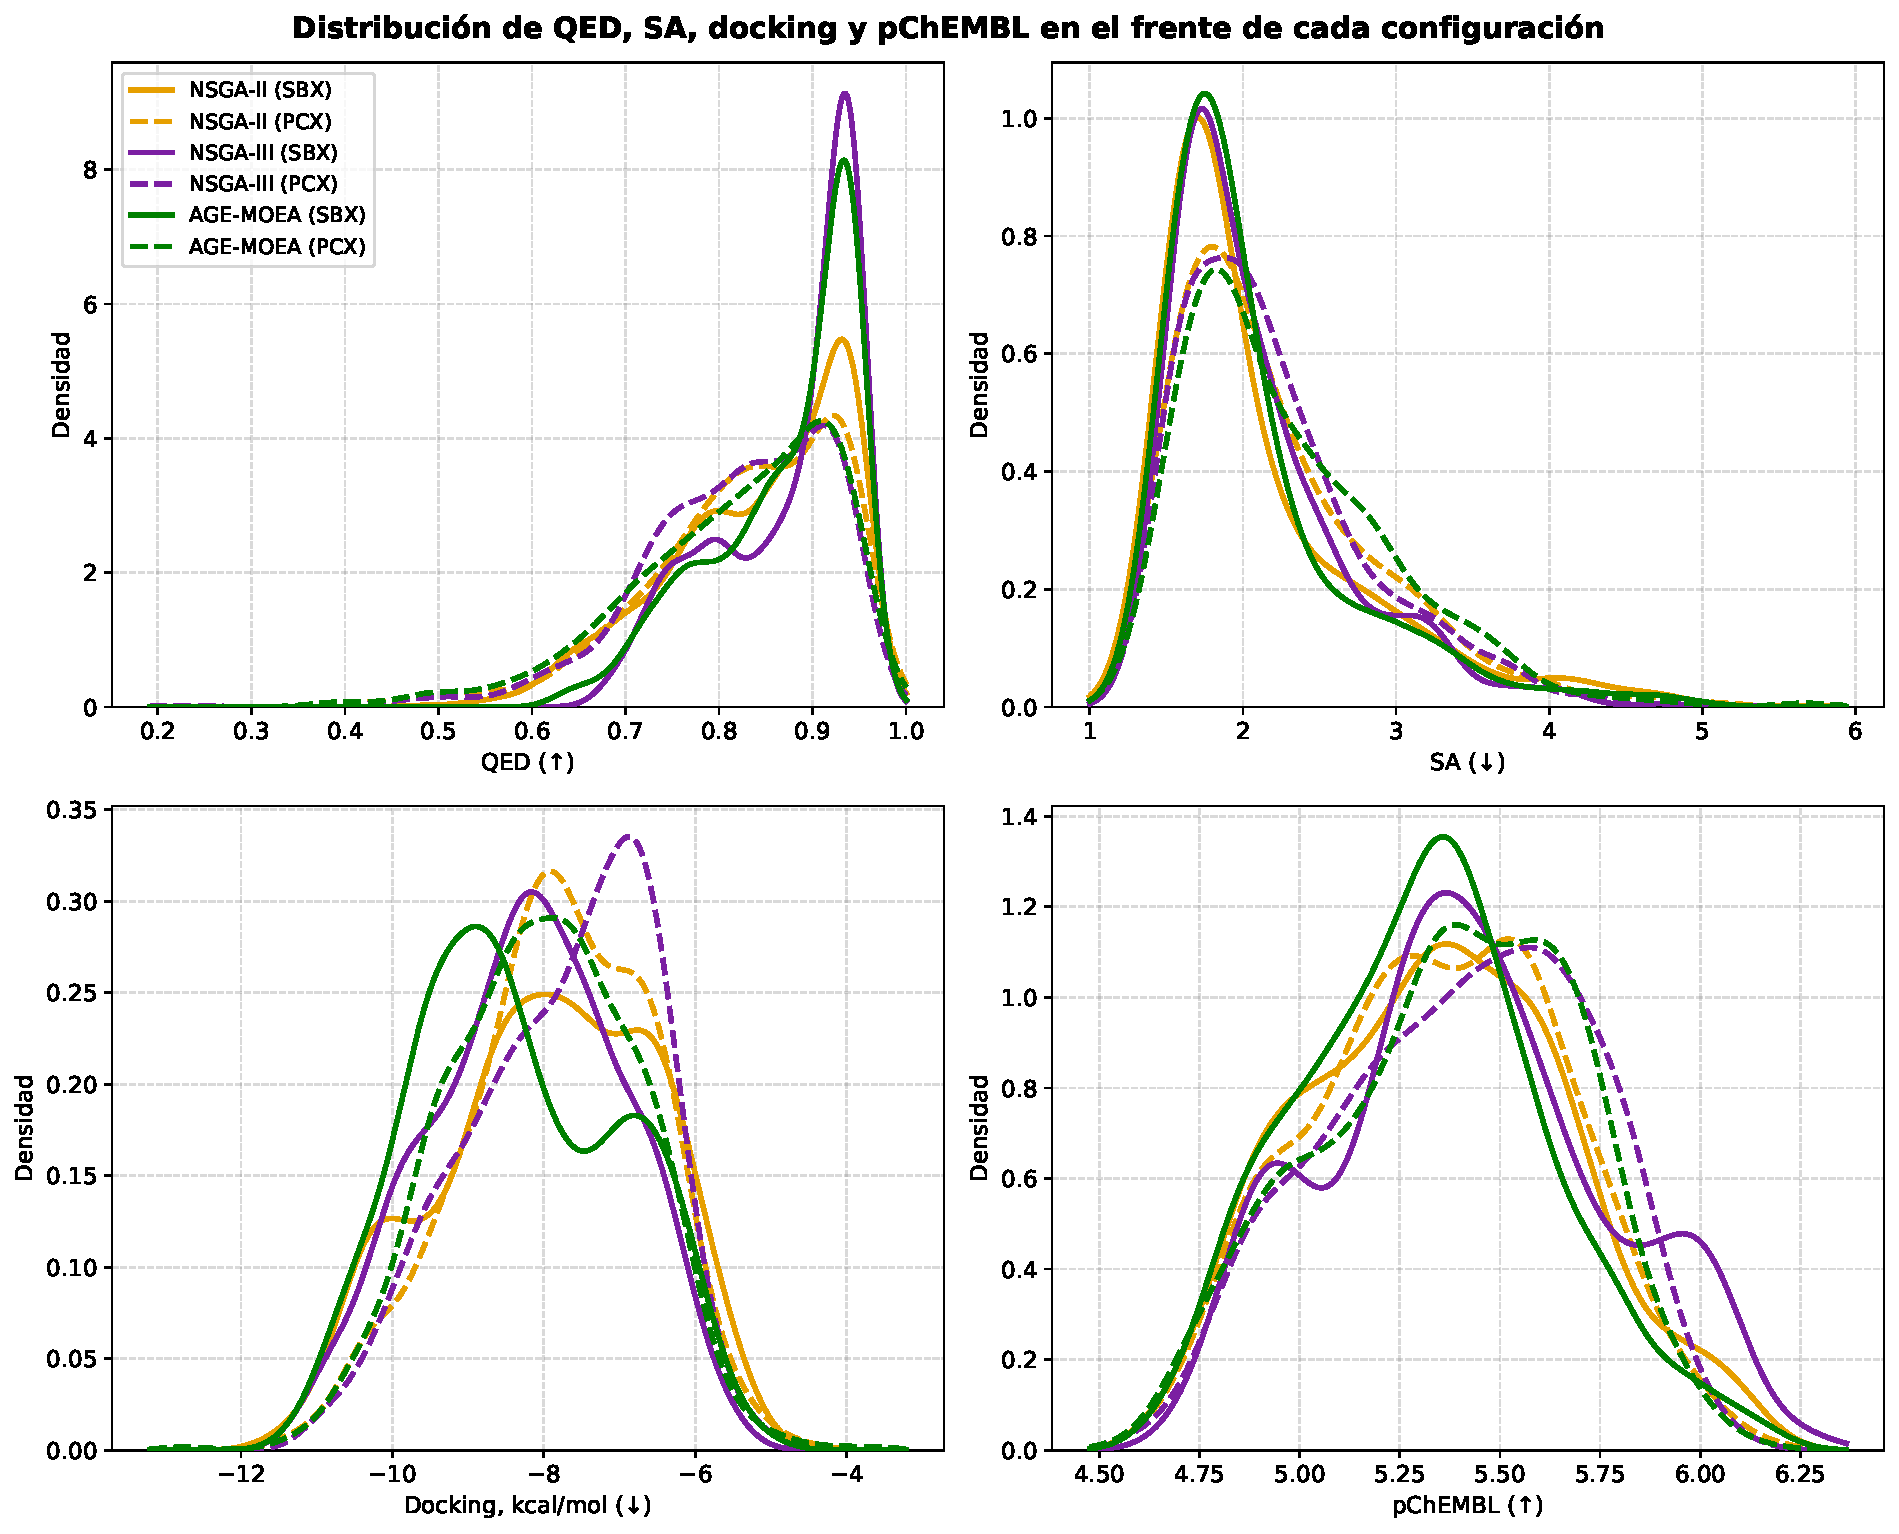
\includegraphics[width=\textwidth]{Figures/mrp1/4_distribucion_propiedades.pdf}
    \caption{Distribución de densidad de los cuatro objetivos de optimización (\gls{qed}, SA, afinidad de unión en kcal/mol y pChEMBL predicho) en el frente no dominado para cada configuración.}
    \label{fig:distribucion_propiedades}
\end{figure}

La Figura~\ref{fig:distribucion_propiedades} muestra la distribución de densidad de los cuatro objetivos de optimización en los frentes obtenidos por cada configuración.

En el gráfico de \gls{qed} se aprecian las tendencias observadas: las variantes con SBX concentran sus soluciones en un pico estrecho y elevado cerca de 0.88--0.94, mientras que PCX dispersa sus moléculas en un rango más amplio con valores menores de \gls{qed}. En la accesibilidad sintética (SA), todos los algoritmos ubican el grueso de sus soluciones en valores favorables (entre 1.8 y 2.5). Al mirar la afinidad de acoplamiento, las curvas de SBX se desplazan hacia energías más negativas, logrando una mayor densidad de soluciones con afinidades entre $-8$ y $-11\text{ kcal/mol}$. Finalmente, en la bioactividad predicha, todas las configuraciones sitúan su distribución por encima del umbral de 5.0, centradas entre 5.25 y 5.50.

\subsubsection{Análisis de Convergencia}
\label{subsubsec:convergencia}

\begin{figure}[H]
    \centering
    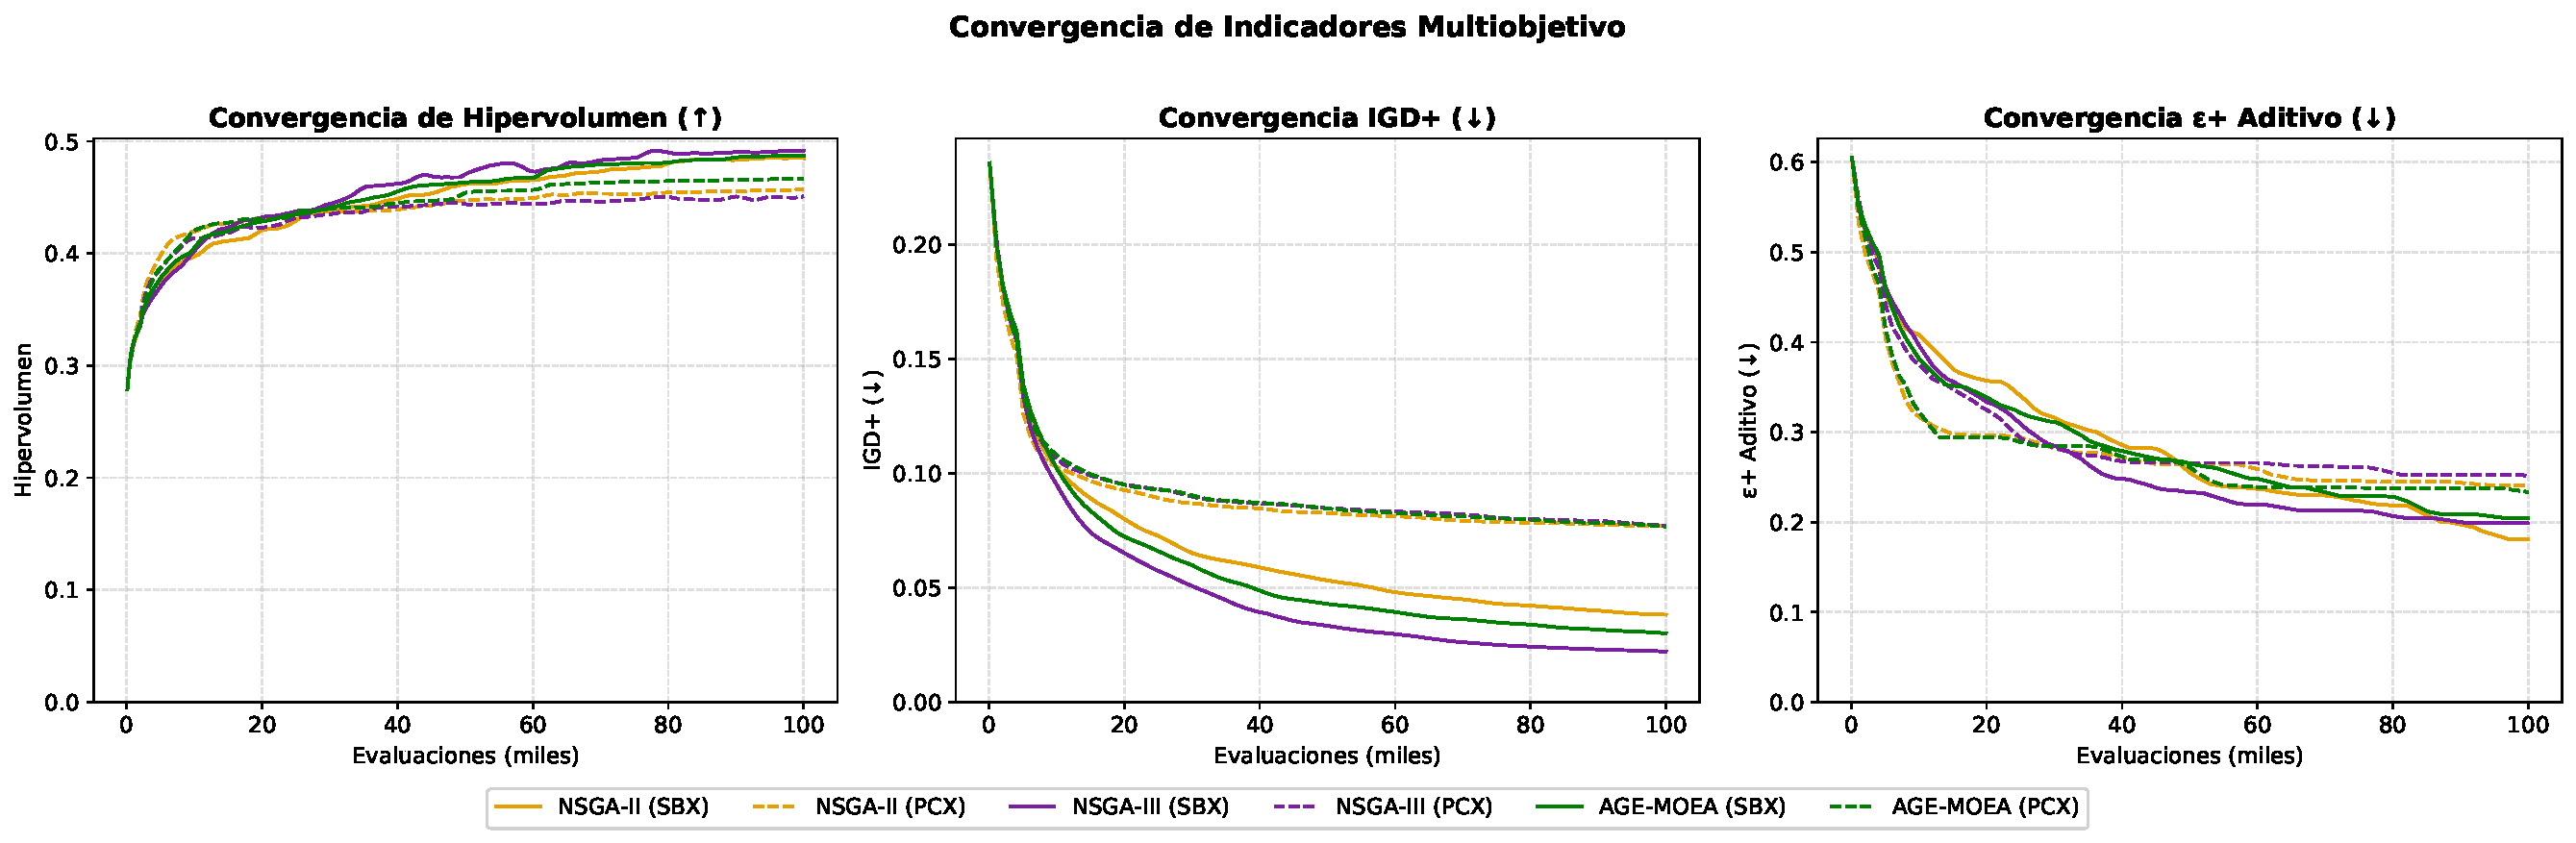
\includegraphics[width=\textwidth]{Figures/mrp1/1_convergencia_multiobjetivo.pdf}
    \caption{Convergencia de los indicadores multiobjetivo en función del número de evaluaciones para cada configuración, promediada sobre las cinco ejecuciones independientes.}
    \label{fig:convergencia_multiobjetivo}
\end{figure}

La Figura~\ref{fig:convergencia_multiobjetivo} muestra la evolución de los indicadores multiobjetivo a lo largo de las 100.000 evaluaciones, promediada sobre las cinco ejecuciones independientes.

En el hipervolumen se observa un crecimiento rápido durante las primeras 20.000 evaluaciones en todas las configuraciones. A partir de esa etapa, \acrshort{nsga3} con SBX presenta un mejor comportamiento y sostiene el valor más alto hasta concluir la búsqueda ($\approx 0.514$). Por su parte, las variantes con PCX se estabilizan alrededor de las 40.000 evaluaciones. La disparidad entre operadores se hace todavía más patente en los indicadores $\text{IGD}^+$ y $\epsilon^+$: aunque todas las configuraciones inician en valores semejantes ($\text{IGD}^+ \approx 0.24$), las variantes con SBX experimentan un descenso abrupto, situándose por debajo de 0.05 antes de las 40.000 evaluaciones, lo cual se traduce en un mejor acercamiento al frente de referencia.

\begin{figure}[H]
    \centering
    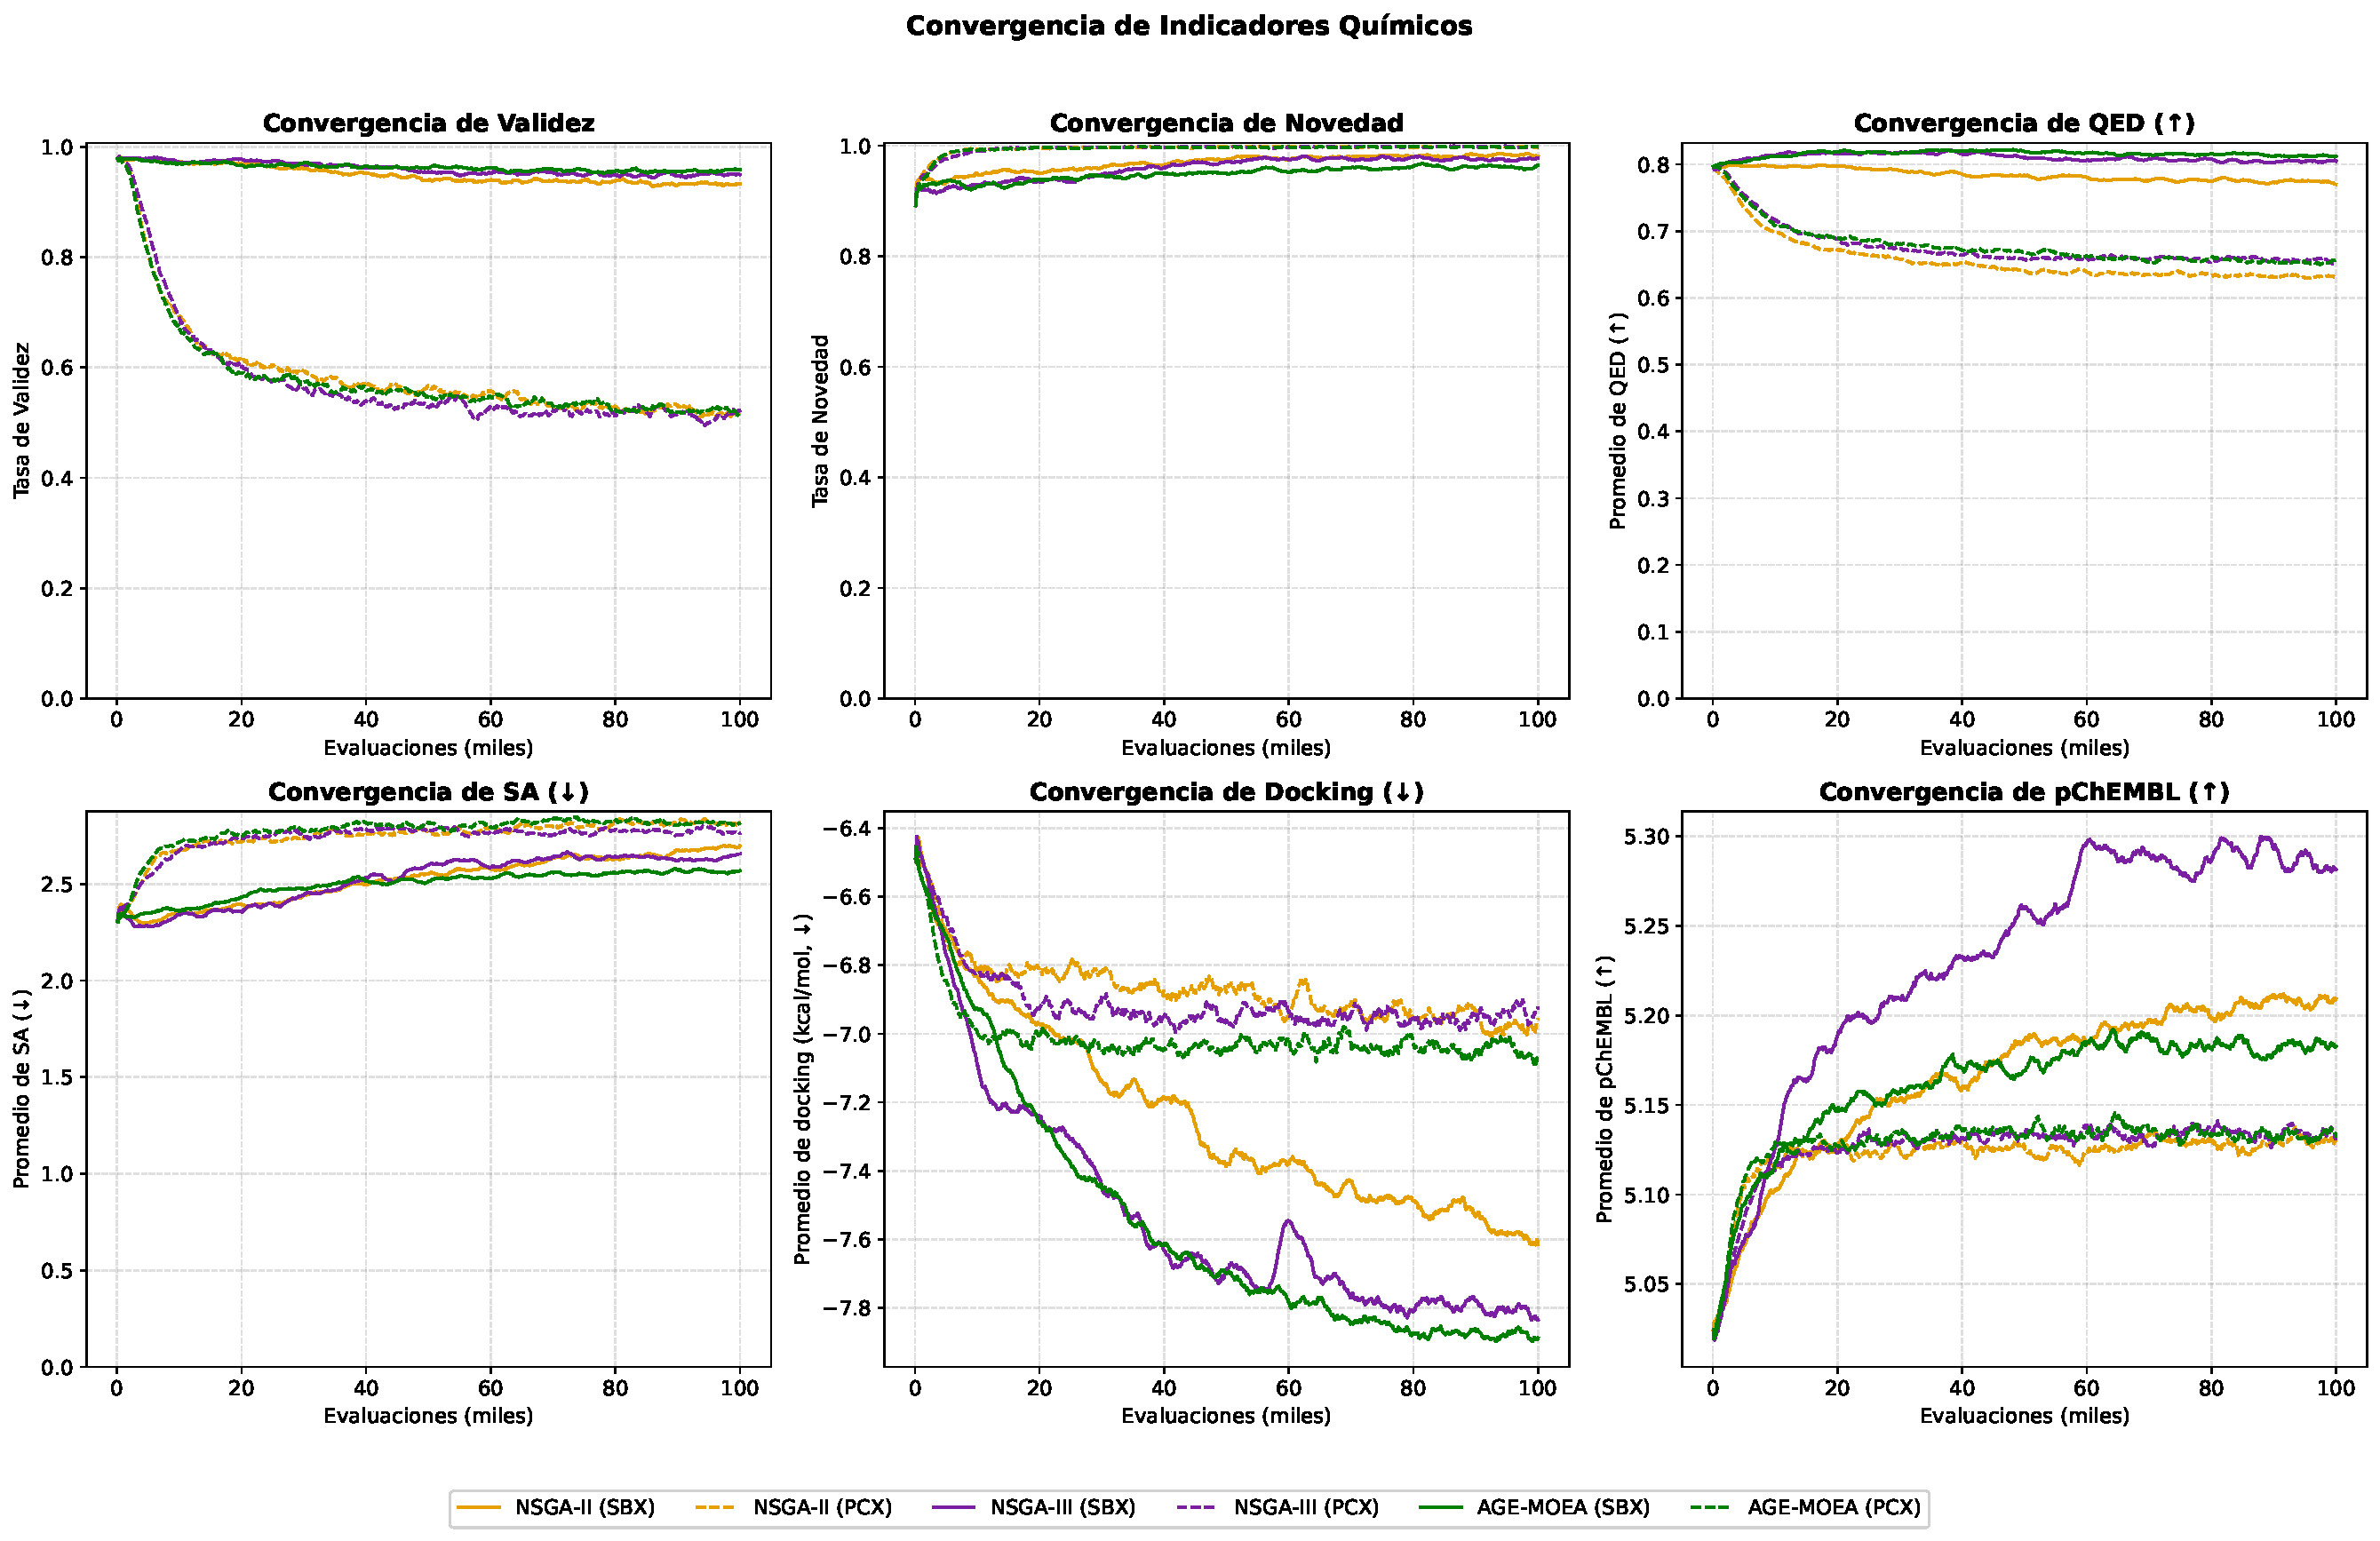
\includegraphics[width=0.98\textwidth]{Figures/mrp1/2_convergencia_quimica.pdf}
    \caption{Evolución y convergencia de las propiedades químicas, validez, novedad, afinidad de unión y pChEMBL predicho a lo largo de las evaluaciones, promediada sobre las cinco ejecuciones independientes.}
    \label{fig:convergencia_quimica}
\end{figure}

La Figura~\ref{fig:convergencia_quimica} presenta la evolución de las métricas de generación y de los cuatro objetivos de optimización a lo largo de la búsqueda.

Las variantes con SBX mantienen una validez química elevada y estable (superior al 94\%--96\%) durante toda la optimización. En cambio, en las configuraciones con PCX la validez cae aceleradamente en las primeras 20.000 evaluaciones. En lo referente a la novedad, todas las variantes exhiben tasas elevadas cercanas a 1.0, con una leve ventaja para las variantes con PCX.

Al analizar la convergencia de los cuatro objetivos, SBX vuelve a presentar un mejor comportamiento. En cuanto a \gls{qed}, las configuraciones con SBX sostienen un promedio superior durante toda la búsqueda. En la afinidad de acoplamiento, las variantes con SBX continúan mejorando de manera sostenida hasta el final, alcanzando \acrshort{nsga3} y \acrshort{agemoea} los valores más bajos, seguidos por \acrshort{nsga2}. Asimismo, la convergencia de pChEMBL muestra que todas las configuraciones inician cerca de 5.0 y progresan hacia valores superiores, destacando \acrshort{nsga3} con SBX al superar consistentemente a sus contrapartes.

\subsubsection{Frentes de Pareto y Frente No Dominado Conjunto Global}
\label{subsubsec:frentes_pareto_mrp1}

\begin{figure}[H]
    \centering
    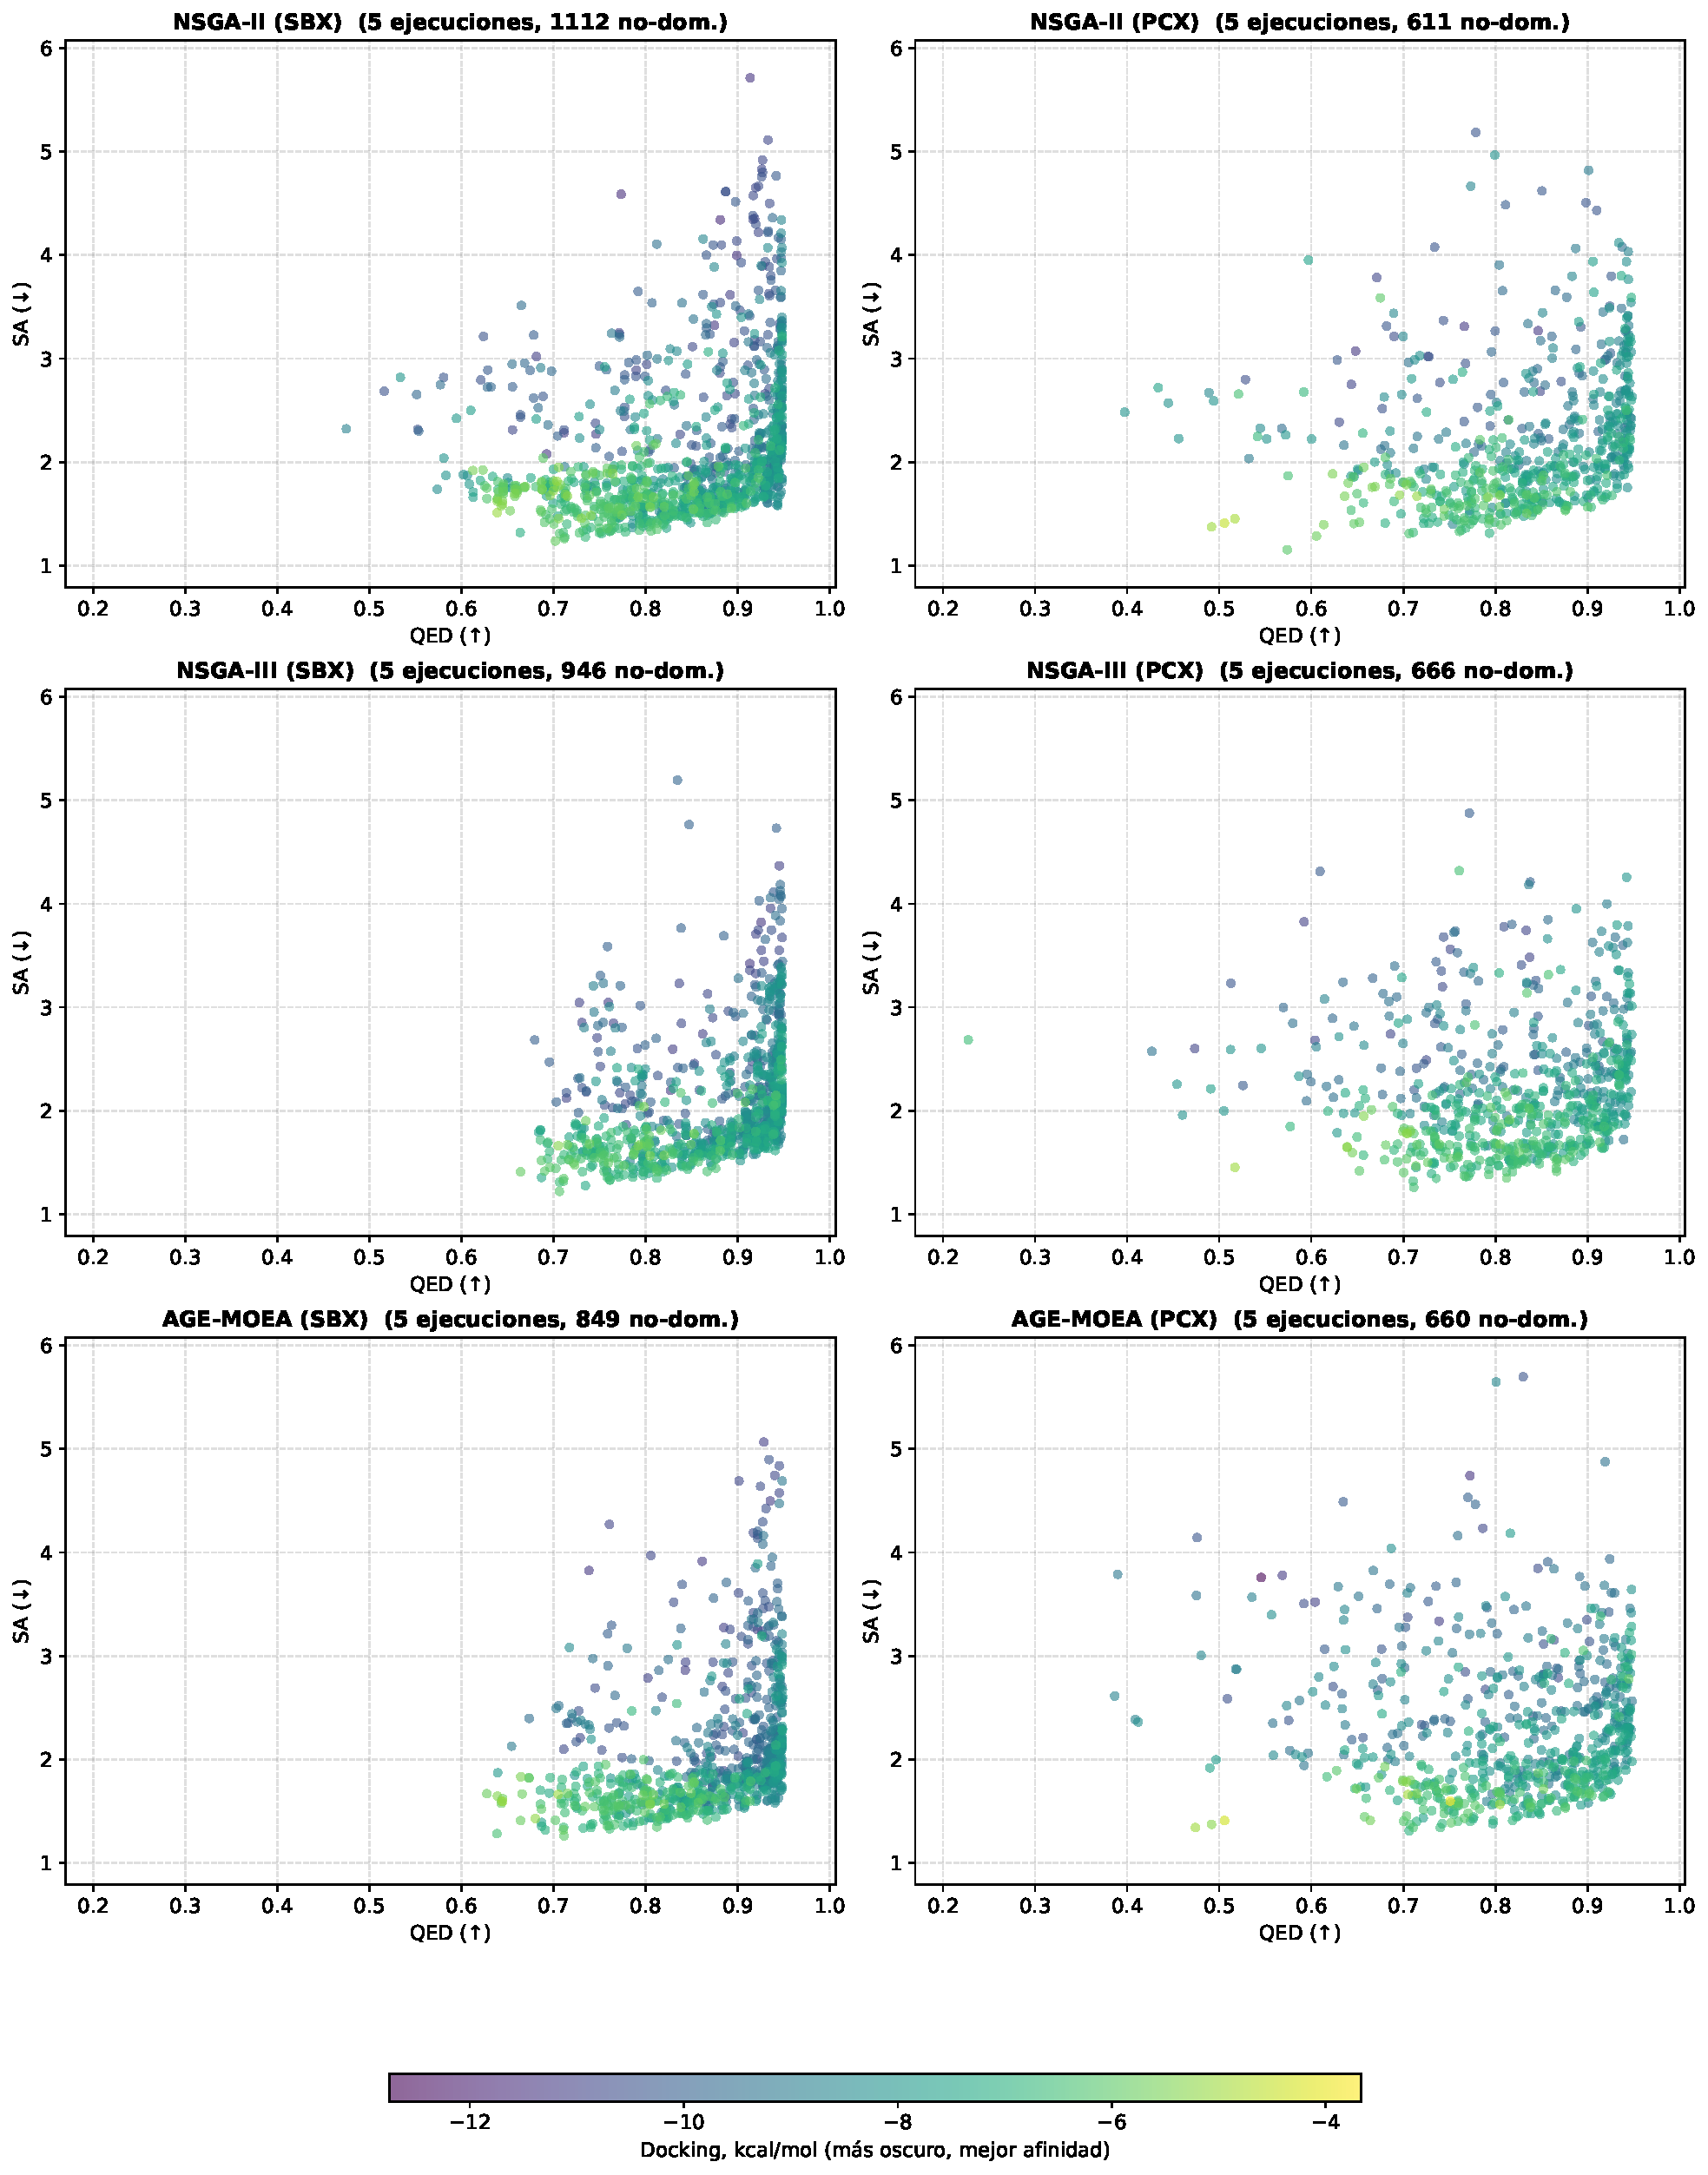
\includegraphics[width=0.95\textwidth]{Figures/mrp1/3_frentes_por_configuracion.pdf}
    \caption{Proyección de los frentes de Pareto en el espacio \gls{qed} vs. SA por configuración para las cinco ejecuciones independientes, con la afinidad de unión indicada mediante la escala de color.}
    \label{fig:frentes_por_configuracion}
\end{figure}

La Figura~\ref{fig:frentes_por_configuracion} presenta los frentes no dominados acumulados en el plano \gls{qed} contra SA para cada configuración sobre las cinco ejecuciones independientes, donde el color de cada punto indica su afinidad de unión hacia \gls{mrp1}.

Se aprecian contrastes definidos entre ambos operadores de cruce. Las variantes con SBX generan frentes con un número considerablemente mayor de soluciones, concentrándose en la región de alto \gls{qed} ($\text{QED} > 0.80$) y bajo SA ($\text{SA} < 2.5$). Además, estas configuraciones concentran una alta proporción de puntos con afinidades muy favorables. Por el contrario, las variantes con PCX dispersan sus soluciones y exploran zonas de menor similitud a fármacos conocidos ($\text{QED} < 0.60$), logrando algunas moléculas con baja complejidad sintética ($\text{SA} \approx 1.2$), pero a expensas de energías de unión menos favorables.

Para evaluar la capacidad exploratoria global, se combinan las soluciones obtenidas por las variantes con PCX y SBX en los tres algoritmos genéticos (\acrshort{nsga2}, \acrshort{nsga3} y \acrshort{agemoea}) a lo largo de las cinco ejecuciones independientes. Se recalcula la no dominancia considerando los cuatro objetivos simultáneos, conformando un Frente No Dominado Conjunto Global de 1396 moléculas únicas.

\begin{figure}[H]
    \centering
    \makebox[\textwidth][c]{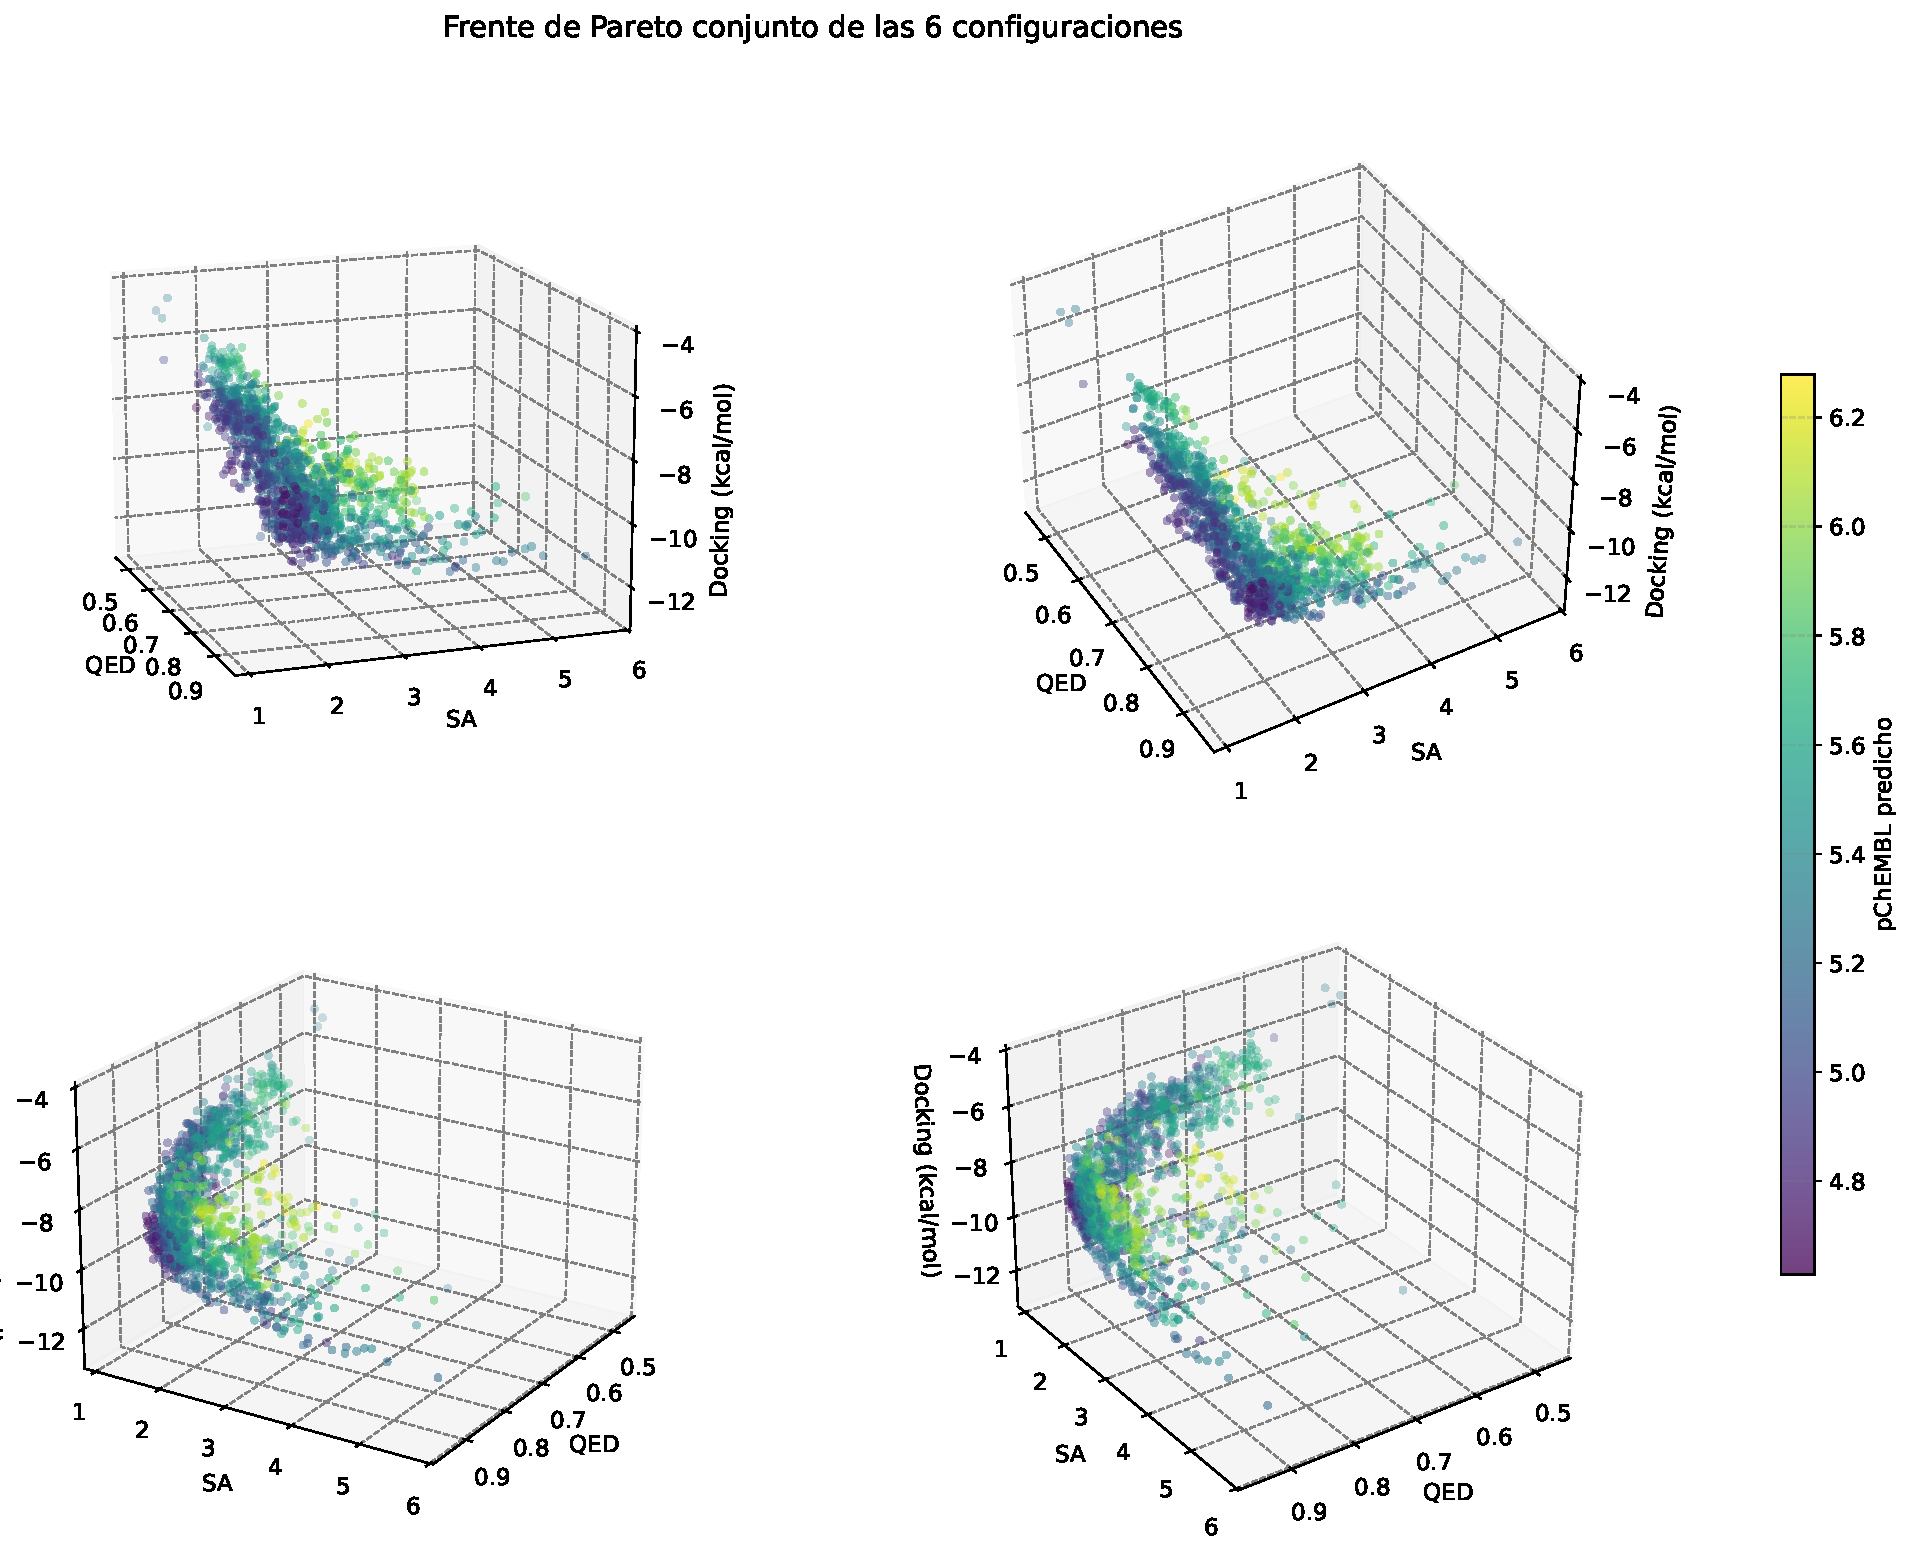
\includegraphics[width=1.05\textwidth]{Figures/mrp1/5_frente_3d_pchembl_conjunto.pdf}}
    \caption{Frente No Dominado Conjunto Global (1396 soluciones) en el espacio tridimensional de objetivos (\gls{qed}, SA y afinidad de docking en kcal/mol), con el valor de pChEMBL predicho indicado mediante la escala de color, visualizado desde cuatro ángulos tridimensionales distintos.}
    \label{fig:frentes_pareto_3d}
\end{figure}

La Figura~\ref{fig:frentes_pareto_3d} muestra el Frente No Dominado Conjunto Global en cuatro perspectivas tridimensionales. En las gráficas se muestra el compromiso entre las propiedades optimizadas: se preserva una alta densidad de moléculas en la franja de alto \gls{qed} ($\text{QED} > 0.85$) y síntesis accesible ($\text{SA} < 2.5$), alcanzando simultáneamente afinidades de acoplamiento por debajo de $-10\text{ kcal/mol}$. La escala de color refleja que al aumentar el valor de accesibilidad sintética también aumenta la afinidad predicha, por lo que el espacio de búsqueda presenta un compromiso entre estos dos objetivos.

En cuanto al aporte de cada método al frente global, los tres algoritmos muestran complementariedad, \acrshort{nsga3} aporta un total de 682 soluciones (525 exclusivas), \acrshort{agemoea} contribuye con 514 soluciones (360 exclusivas) y \acrshort{nsga2} provee 464 soluciones (303 exclusivas). Asimismo, 205 moléculas (un 14.7\% del frente) fueron descubiertas conjuntamente por más de un algoritmo.

% -----------------------------------------------------------------------------
\subsection{Comparación con Modelos de Referencia}
\label{subsec:comp_estado_arte_mrp1}
\label{sec:comparacion_referencia}

Se comparó el enfoque multiobjetivo propuesto con modelos generativos de referencia entrenados con \gls{moses}:

\begin{itemize}
    \item \textbf{\gls{vae}:} El \gls{vae} utilizado en el modelo propuesto, entrenado con \gls{moses}.
    \item \textbf{\gls{vae} con fine-tuning:} El mismo \gls{vae} ajustado mediante fine-tuning con ligandos conocidos asociados a \gls{mrp1} para sesgar la generación hacia la diana.
    \item \textbf{GAN:} Red generativa adversaria del benchmark \gls{moses} (LatentGAN).
    \item \textbf{GAN con fine-tuning:} La misma GAN ajustada con ligandos conocidos de \gls{mrp1}.
\end{itemize}

De cada modelo de referencia se generaron 100.000 moléculas al azar y se evaluó una muestra de 10.000 cumpliendo $F_{\text{sp3}} \ge 0.3$ en \gls{qed}, SA, afinidad de docking con Uni-Dock y pChEMBL predicho. En la Tabla~\ref{tab:comparacion_modelos} se contrastan directamente las seis configuraciones multiobjetivo del presente estudio con los cuatro modelos generativos de referencia.

\begin{table}[htbp]
\centering
\caption{Comparación con los modelos generativos de referencia.}
\label{tab:comparacion_modelos}
\resizebox{\textwidth}{!}{
\begin{tabular}{lccccccc}
\toprule
Modelo & QED $\uparrow$ & SA $\downarrow$ & Docking $\downarrow$ & pChEMBL $\uparrow$ & Validez $\uparrow$ & Unicidad $\uparrow$ & Novedad $\uparrow$ \\
\midrule
N2-SBX & $0.840 \pm 0.015$ & $2.152 \pm 0.069$ & $-7.878 \pm 0.151$ & $5.341 \pm 0.034$ & $0.949 \pm 0.015$ & $0.996 \pm 0.010$ & $0.969 \pm 0.011$ \\
N2-PCX & $0.798 \pm 0.012$ & $2.299 \pm 0.027$ & $-7.802 \pm 0.071$ & $5.345 \pm 0.016$ & $0.583 \pm 0.015$ & $\mathbf{1.000 \pm 0.000}$ & $\mathbf{0.995 \pm 0.001}$ \\
N3-SBX & $\mathbf{0.870 \pm 0.009}$ & $2.170 \pm 0.078$ & $-8.182 \pm 0.079$ & $\mathbf{5.397 \pm 0.038}$ & $0.960 \pm 0.009$ & $0.985 \pm 0.016$ & $0.960 \pm 0.008$ \\
N3-PCX & $0.809 \pm 0.016$ & $2.292 \pm 0.043$ & $-7.781 \pm 0.023$ & $5.352 \pm 0.022$ & $0.570 \pm 0.010$ & $\mathbf{1.000 \pm 0.000}$ & $0.994 \pm 0.001$ \\
AGE-SBX & $0.868 \pm 0.009$ & $\mathbf{2.115 \pm 0.126}$ & $-8.093 \pm 0.138$ & $5.318 \pm 0.073$ & $0.963 \pm 0.009$ & $0.992 \pm 0.008$ & $0.949 \pm 0.013$ \\
AGE-PCX & $0.808 \pm 0.011$ & $2.335 \pm 0.051$ & $-7.884 \pm 0.029$ & $5.354 \pm 0.024$ & $0.576 \pm 0.027$ & $\mathbf{1.000 \pm 0.000}$ & $0.994 \pm 0.002$ \\
\midrule
VAE & $0.800 \pm 0.097$ & $2.517 \pm 0.506$ & $-7.688 \pm 0.772$ & $5.084 \pm 0.203$ & $\mathbf{0.974}$ & $0.999$ & $0.938$ \\
VAE-ft & $0.640 \pm 0.162$ & $2.659 \pm 0.548$ & $\mathbf{-8.339 \pm 0.900}$ & $5.111 \pm 0.215$ & $0.858$ & $\mathbf{1.000}$ & $0.991$ \\
GAN & $0.795 \pm 0.101$ & $2.528 \pm 0.563$ & $-7.663 \pm 0.819$ & $5.053 \pm 0.199$ & $0.875$ & $0.984$ & $0.960$ \\
GAN-ft & $0.632 \pm 0.174$ & $2.758 \pm 0.737$ & $-8.323 \pm 1.024$ & $5.139 \pm 0.273$ & $0.663$ & $0.990$ & $0.992$ \\
\bottomrule
\end{tabular}
}
\end{table}



Como se observa en la Tabla~\ref{tab:comparacion_modelos}, los enfoques multiobjetivo propuestos superan de manera categórica a los modelos generativos de referencia en el balance global de propiedades farmacológicas. En particular, \acrshort{nsga3} (SBX) logra el mayor valor promedio de \gls{qed} ($0.870 \pm 0.009$), una afinidad de docking sólida ($-8.182 \pm 0.079\text{ kcal/mol}$) y la mayor predicción de bioactividad ($5.397 \pm 0.038$), preservando una validez sobresaliente del $96.0\%$, unicidad del $98.5\%$ y novedad del $96.0\%$. Asimismo, \acrshort{agemoea} (SBX) consigue la mejor accesibilidad sintética global ($\text{SA} = 2.115 \pm 0.126$), mientras que las variantes con PCX exhiben una unicidad perfecta del $100.0\%$ y novedades de hasta $99.5\%$, si bien a expensas de una menor tasa de validez química ($57.0\% - 58.3\%$).

En los modelos generativos de referencia no guiados (\gls{vae} y GAN base), el \gls{qed} ronda $0.795 - 0.800$, pero las afinidades de unión resultan más débiles ($-7.66$ a $-7.69\text{ kcal/mol}$) y la bioactividad promedio apenas roza el umbral de corte ($\text{pChEMBL} \approx 5.05 - 5.08$). El ajuste por fine-tuning incrementa la afinidad hacia la diana ($-8.34\text{ kcal/mol}$ en \gls{vae} y $-8.32\text{ kcal/mol}$ en GAN) y eleva discretamente el pChEMBL ($5.11 - 5.14$), pero provoca un severo detrimento en el valor de \gls{qed} (descendiendo a $0.63 - 0.64$), incrementa la dificultad sintética ($\text{SA} > 2.65$) y degrada notablemente la validez química en la GAN hasta un $66.3\%$.

En conjunto, estos contrastes confirman que la optimización multiobjetivo en el espacio latente es capaz de enriquecer simultáneamente la potencia biológica y la afinidad de unión hacia \gls{mrp1} sin sacrificar el \gls{qed} ni la accesibilidad sintética de las moléculas generadas.

% -----------------------------------------------------------------------------
\subsection{Validación y Perfilado de las Moléculas Candidatas}
\label{subsec:mejores_moleculas}
\label{sec:validacion_perfilado}

Con el fin de evaluar y caracterizar las moléculas obtenidas para \gls{mrp1}, se realiza un análisis sobre las soluciones del frente de Pareto de cada configuración y los modelos de referencia. Esta sección examina la calidad física de las conformaciones de acoplamiento mediante PoseBusters \cite{buttenschoen2024posebusters}, la potencia y bioactividad inhibitoria predicha con Random Forest a partir de ChEMBL \cite{mendez2019chembl}, y el perfil farmacocinético, fisicoquímico y toxicológico mediante ADMET-AI \cite{swanson2024admetai}.

\subsubsection{Moléculas Representativas}
\label{subsubsec:moleculas_representativas}
\label{subsec:moleculas_candidatas}

Con el fin de analizar las moléculas generadas con un perfil equilibrado, se aplicó un filtrado sobre el Frente No Dominado Conjunto Global seleccionando aquellas que satisfacen simultáneamente condiciones en los cuatro objetivos: $\text{Docking} < -10\text{ kcal/mol}$, $\text{pChEMBL} > 5.5$, $\text{QED} > 0.70$ y $\text{SA} < 3.0$.

\begin{figure}[H]
    \centering
    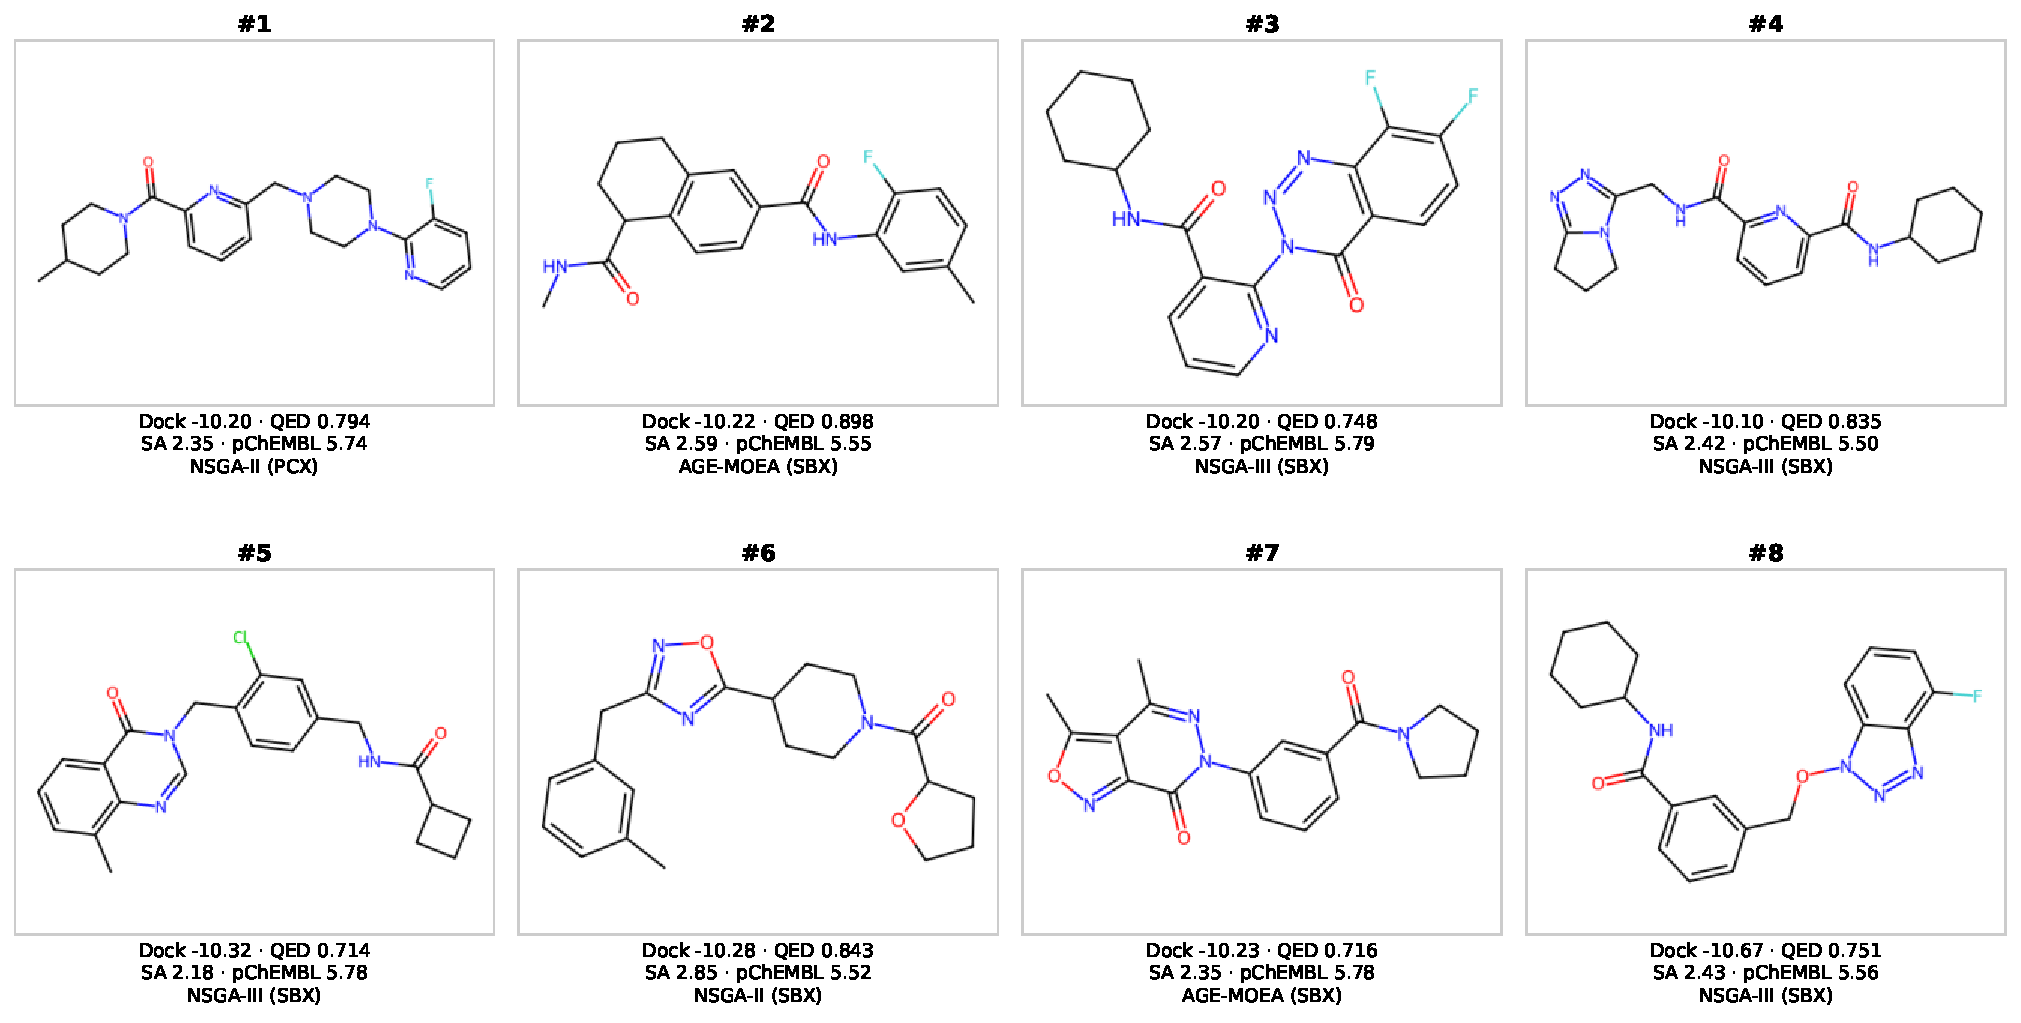
\includegraphics[width=\textwidth]{Figures/mrp1/moleculas_candidatas.pdf}
    \caption{Estructuras químicas y propiedades de las ocho moléculas seleccionadas del Frente No Dominado Conjunto Global ($\text{Docking} < -10\text{ kcal/mol}$, $\text{pChEMBL} > 5.5$, $\text{QED} > 0.70$ y $\text{SA} < 3.0$).}
    \label{fig:moleculas_candidatas}
\end{figure}

\begin{table}[htbp]
\centering
\caption{Propiedades de las ocho moléculas seleccionadas del Frente No Dominado Conjunto Global.}
\label{tab:moleculas_candidatas}
\resizebox{\textwidth}{!}{
\begin{tabular}{clcccccc}
\toprule
Rank & Algoritmo & QED $\uparrow$ & SA $\downarrow$ & Docking (kcal/mol) $\downarrow$ & pChEMBL $\uparrow$ & $\log P$ & $F_{\text{sp3}}$ \\
\midrule
1 & NSGA-II (PCX) & 0,794 & 2,35 & $-10.20$ & 5,74 & 2,81 & 0,50 \\
2 & AGE-MOEA (SBX) & 0,898 & 2,59 & $-10.22$ & 5,55 & 3,55 & 0,30 \\
3 & NSGA-III (SBX) & 0,748 & 2,57 & $-10.20$ & 5,79 & 2,52 & 0,32 \\
4 & NSGA-III (SBX) & 0,835 & 2,42 & $-10.10$ & 5,50 & 1,61 & 0,53 \\
5 & NSGA-III (SBX) & 0,714 & 2,18 & $-10.32$ & 5,78 & 3,82 & 0,32 \\
6 & NSGA-II (SBX) & 0,843 & 2,85 & $-10.28$ & 5,52 & 2,85 & 0,55 \\
7 & AGE-MOEA (SBX) & 0,716 & 2,35 & $-10.23$ & 5,78 & 2,23 & 0,33 \\
8 & NSGA-III (SBX) & 0,751 & 2,43 & $-10.67$ & 5,56 & 3,26 & 0,35 \\
\bottomrule
\end{tabular}
}
\end{table}


La Figura~\ref{fig:moleculas_candidatas} y la Tabla~\ref{tab:moleculas_candidatas} presentan las ocho moléculas seleccionadas a partir de este filtrado. Las soluciones provienen de distintas configuraciones algorítmicas, principalmente de las variantes con SBX en \acrshort{nsga3} y \acrshort{agemoea}, junto con aportes de \acrshort{nsga2}. A nivel estructural, estas moléculas presentan una mayor complejidad, combinando múltiples anillos aromáticos y grupos funcionales que permiten mantener un equilibrio entre \gls{qed}, facilidad de síntesis y afinidad hacia la diana.

En comparación con las moléculas del experimento previo sin diana (Sección~\ref{sec:res_genericos}), donde solo se optimizaban \gls{qed} y SA, la incorporación del acoplamiento molecular y la bioactividad hacia \gls{mrp1} conduce a estructuras de mayor tamaño y complejidad. Mientras que en el caso previo se favorecían moléculas más pequeñas o simples, aquí la necesidad de interactuar con la cavidad de la proteína promueve la presencia de más anillos aromáticos y grupos que permitan formar interacciones en el sitio de unión, conservando al mismo tiempo una síntesis accesible y cumpliendo las restricciones fisicoquímicas.

\subsubsection{Validación de Poses de Acoplamiento (PoseBusters)}
\label{subsubsec:posebusters}

Para verificar la viabilidad física de las conformaciones tridimensionales generadas por acoplamiento molecular en la cavidad de \gls{mrp1}, se empleó PoseBusters \cite{buttenschoen2024posebusters}. Esta herramienta somete cada complejo ligando-proteína a 20 pruebas independientes que evalúan la química básica del ligando y la interacción física con el receptor. La métrica evaluada corresponde a la tasa de validez física sobre el conjunto de las 100 mejores moléculas de cada método.

\begin{figure}[H]
    \centering
    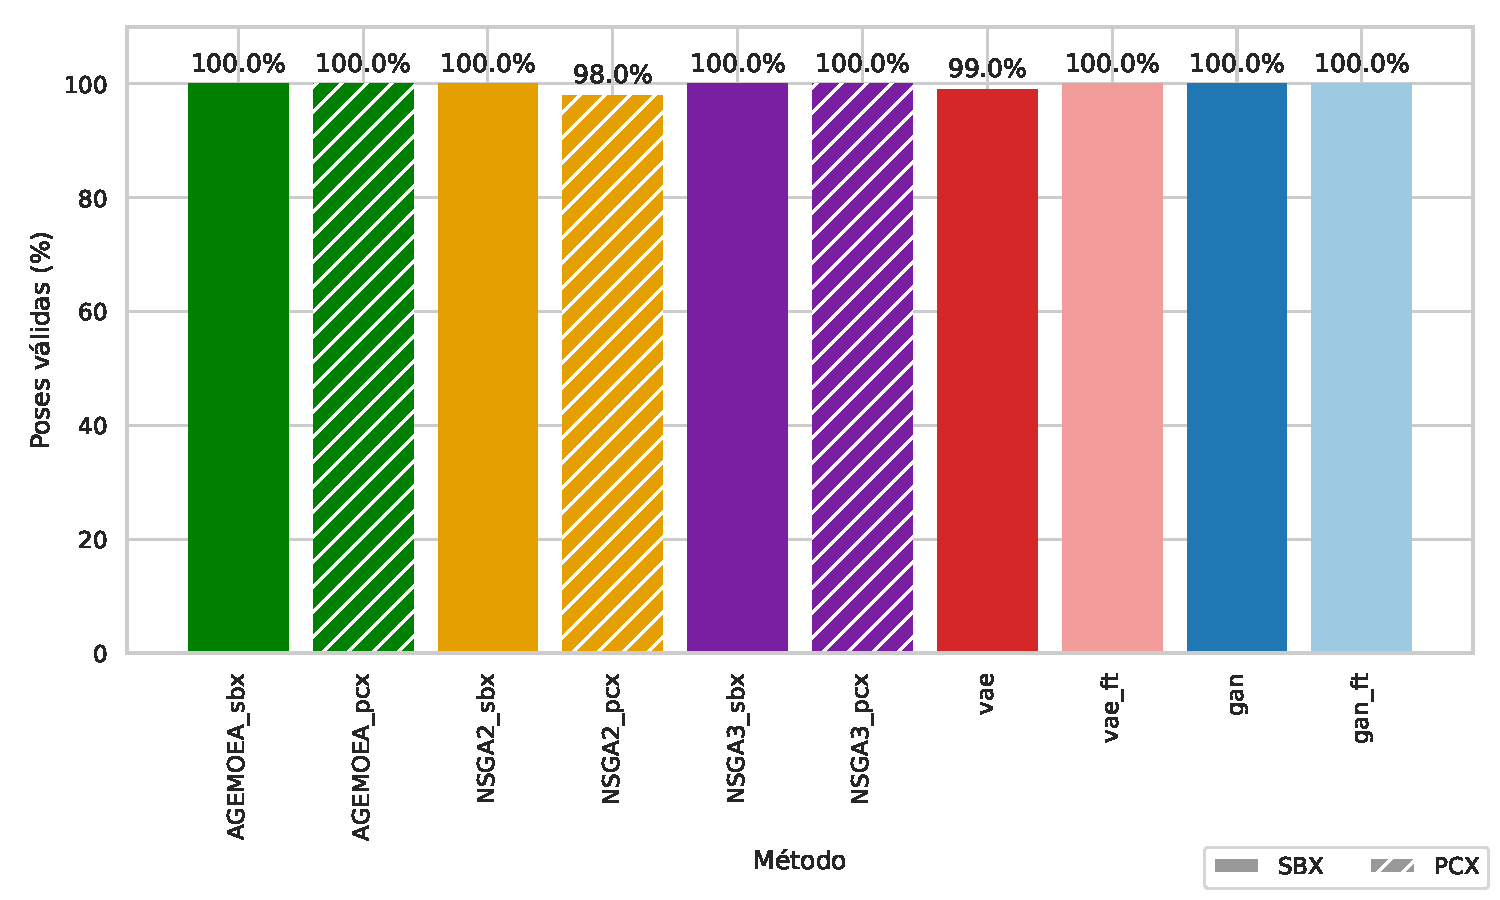
\includegraphics[width=0.85\textwidth]{Figures/mrp1/posebuster.pdf}
    \caption{Tasa de validez de PoseBusters en el top 100 de moléculas para cada variante algorítmica y modelo de referencia.}
    \label{fig:posebusters}
\end{figure}

Como se observa en la Figura~\ref{fig:posebusters}, todas las configuraciones multiobjetivo y los modelos de referencia alcanzan entre un 98\% y un 100\% de validez en las 20 pruebas de PoseBusters. Estos resultados confirman que las conformaciones predichas por acoplamiento molecular son físicamente viables y respetan la geometría del sitio de unión en \gls{mrp1}, sin presentar choques entre átomos ni distorsiones estructurales.

\subsubsection{Predicción de Potencia y Bioactividad Inhibitoria}
\label{subsubsec:potencia_bioactividad}

La bioactividad frente a \gls{mrp1} se evaluó mediante un modelo de Random Forest entrenado con inhibidores de ChEMBL \cite{mendez2019chembl}. Como métrica se utiliza el valor de pChEMBL predicho, fijando un umbral de $5.0$ para considerar activo al compuesto ($\text{IC}_{50} \le 10\,\mu\text{M}$).

\begin{figure}[H]
    \centering
    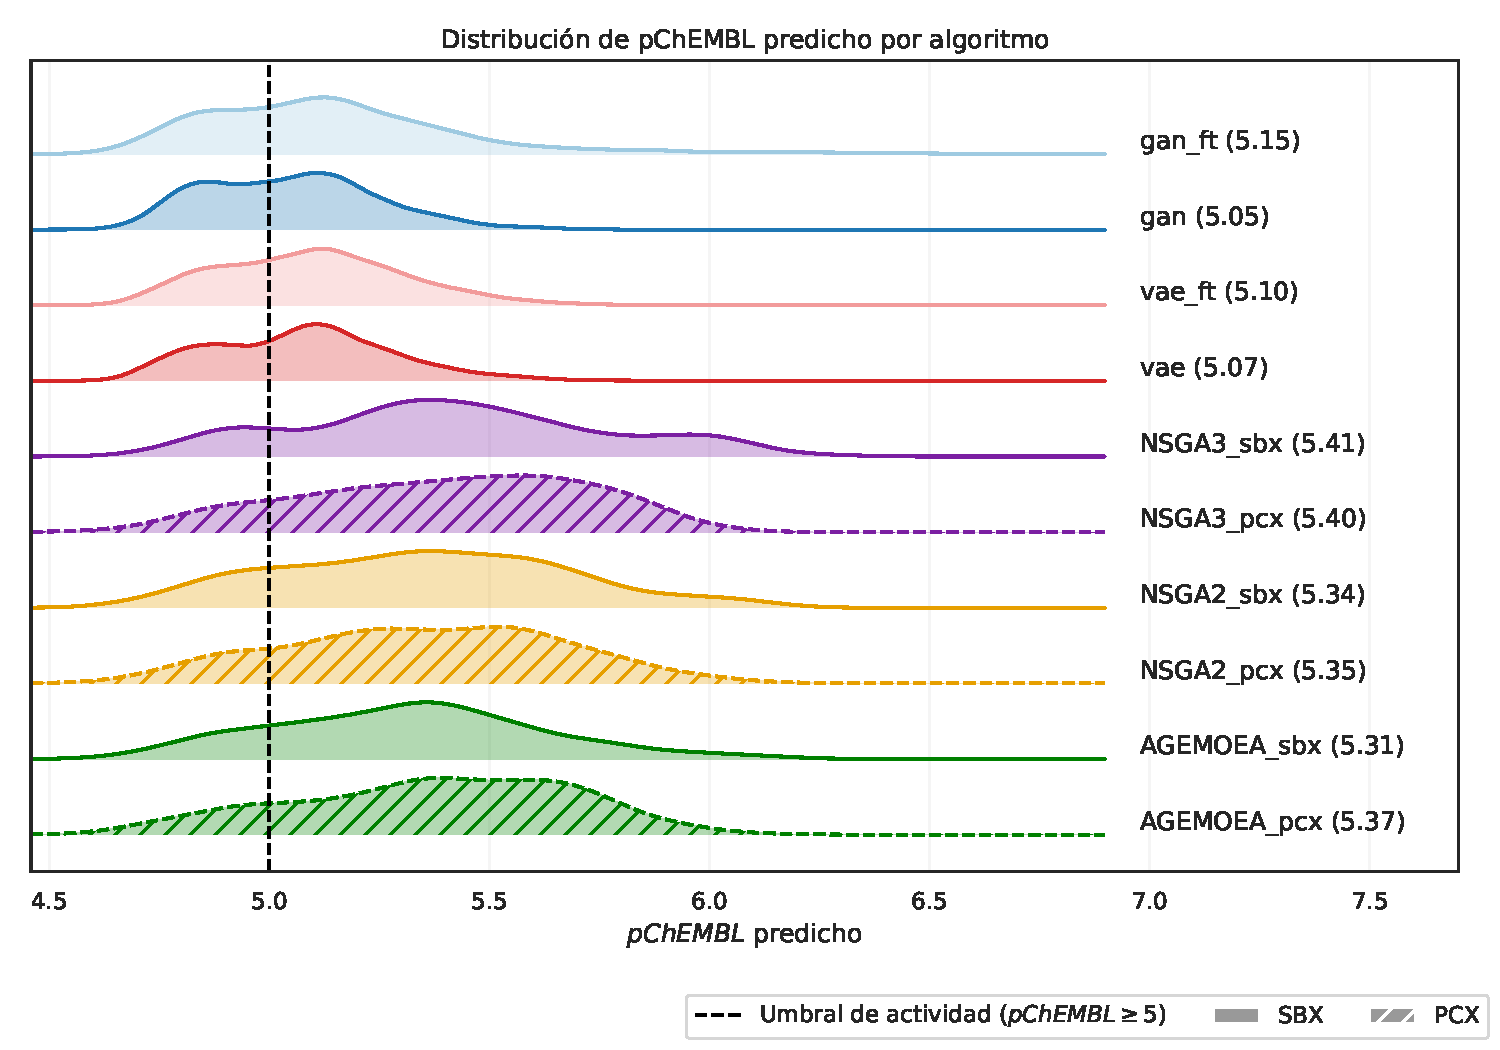
\includegraphics[width=0.88\textwidth]{Figures/mrp1/pchembl.pdf}
    \caption{Distribución de densidad (KDE) del valor pChEMBL predicho para cada algoritmo y modelo de referencia. La línea vertical discontinua indica el umbral de actividad biológica ($\text{pChEMBL} \ge 5.0$).}
    \label{fig:distribucion_pchembl}
\end{figure}

\begin{table}[htbp]
\centering
\caption{Estadísticos descriptivos del pChEMBL predicho por configuración.}
\label{tab:pchembl_predicho}
\begin{tabular}{lcccccccc}
\toprule
Configuración & Moléculas & Media & Desv. & Mín. & Q1 & Mediana & Q3 & Máx. \\
\midrule
NSGA-II (SBX) & $1112$ & $5.344$ & $0.326$ & $4.628$ & $5.087$ & $5.348$ & $5.581$ & $6.178$ \\
NSGA-II (PCX) & $611$ & $5.348$ & $0.310$ & $4.573$ & $5.125$ & $5.342$ & $5.578$ & $6.167$ \\
NSGA-III (SBX) & $946$ & $5.413$ & $0.344$ & $4.682$ & $5.192$ & $5.391$ & $5.629$ & $6.279$ \\
NSGA-III (PCX) & $666$ & $5.396$ & $0.315$ & $4.582$ & $5.161$ & $5.425$ & $5.643$ & $6.069$ \\
AGE-MOEA (SBX) & $849$ & $5.311$ & $0.304$ & $4.631$ & $5.087$ & $5.320$ & $5.503$ & $6.179$ \\
AGE-MOEA (PCX) & $660$ & $5.370$ & $0.311$ & $4.562$ & $5.141$ & $5.391$ & $5.616$ & $6.140$ \\
\midrule
VAE & $9991$ & $5.075$ & $0.206$ & $4.537$ & $4.914$ & $5.078$ & $5.205$ & $5.875$ \\
VAE con fine-tuning & $9982$ & $5.099$ & $0.218$ & $4.534$ & $4.935$ & $5.095$ & $5.237$ & $6.875$ \\
GAN & $9988$ & $5.049$ & $0.198$ & $4.503$ & $4.890$ & $5.047$ & $5.178$ & $5.953$ \\
GAN con fine-tuning & $9936$ & $5.149$ & $0.313$ & $4.460$ & $4.929$ & $5.112$ & $5.292$ & $6.897$ \\
\bottomrule
\end{tabular}
\end{table}


La Figura~\ref{fig:distribucion_pchembl} y la Tabla~\ref{tab:pchembl_predicho} presentan los estadísticos descriptivos y las funciones de densidad del pChEMBL predicho sobre las moléculas generadas por cada método.

Como se observa, todas las configuraciones multiobjetivo desplazan su distribución por encima del umbral de 5.0, logrando que la gran mayoría de las moléculas generadas sean predichas como activas. Entre los algoritmos evaluados, \acrshort{nsga3} presenta los valores promedio más altos de bioactividad (tanto con SBX como con PCX) y alcanza el valor máximo del conjunto cercano a 6.28 en su variante con SBX, seguido de cerca por \acrshort{agemoea} y \acrshort{nsga2}.

En cambio, los modelos de referencia (tanto base como con fine-tuning) concentran gran parte de sus soluciones alrededor o por debajo del umbral, produciendo una proporción importante de compuestos inactivos. Esto confirma que la optimización guiada en el espacio latente favorece de forma efectiva la obtención de moléculas activas frente a \gls{mrp1}.

\subsubsection{Perfil Farmacocinético, Fisicoquímico y Toxicológico (\texorpdfstring{\gls{admet}}{ADMET})}
\label{subsubsec:perfil_admet}

El perfil \gls{admet} de las moléculas candidatas se caracterizó utilizando ADMET-AI \cite{swanson2024admetai}, basado en modelos de aprendizaje automático de Therapeutics Data Commons. Se estudiaron descriptores agrupados en tres dimensiones clave: absorción y permeabilidad, fisicoquímica y toxicidad/seguridad.

\begin{figure}[H]
    \centering
    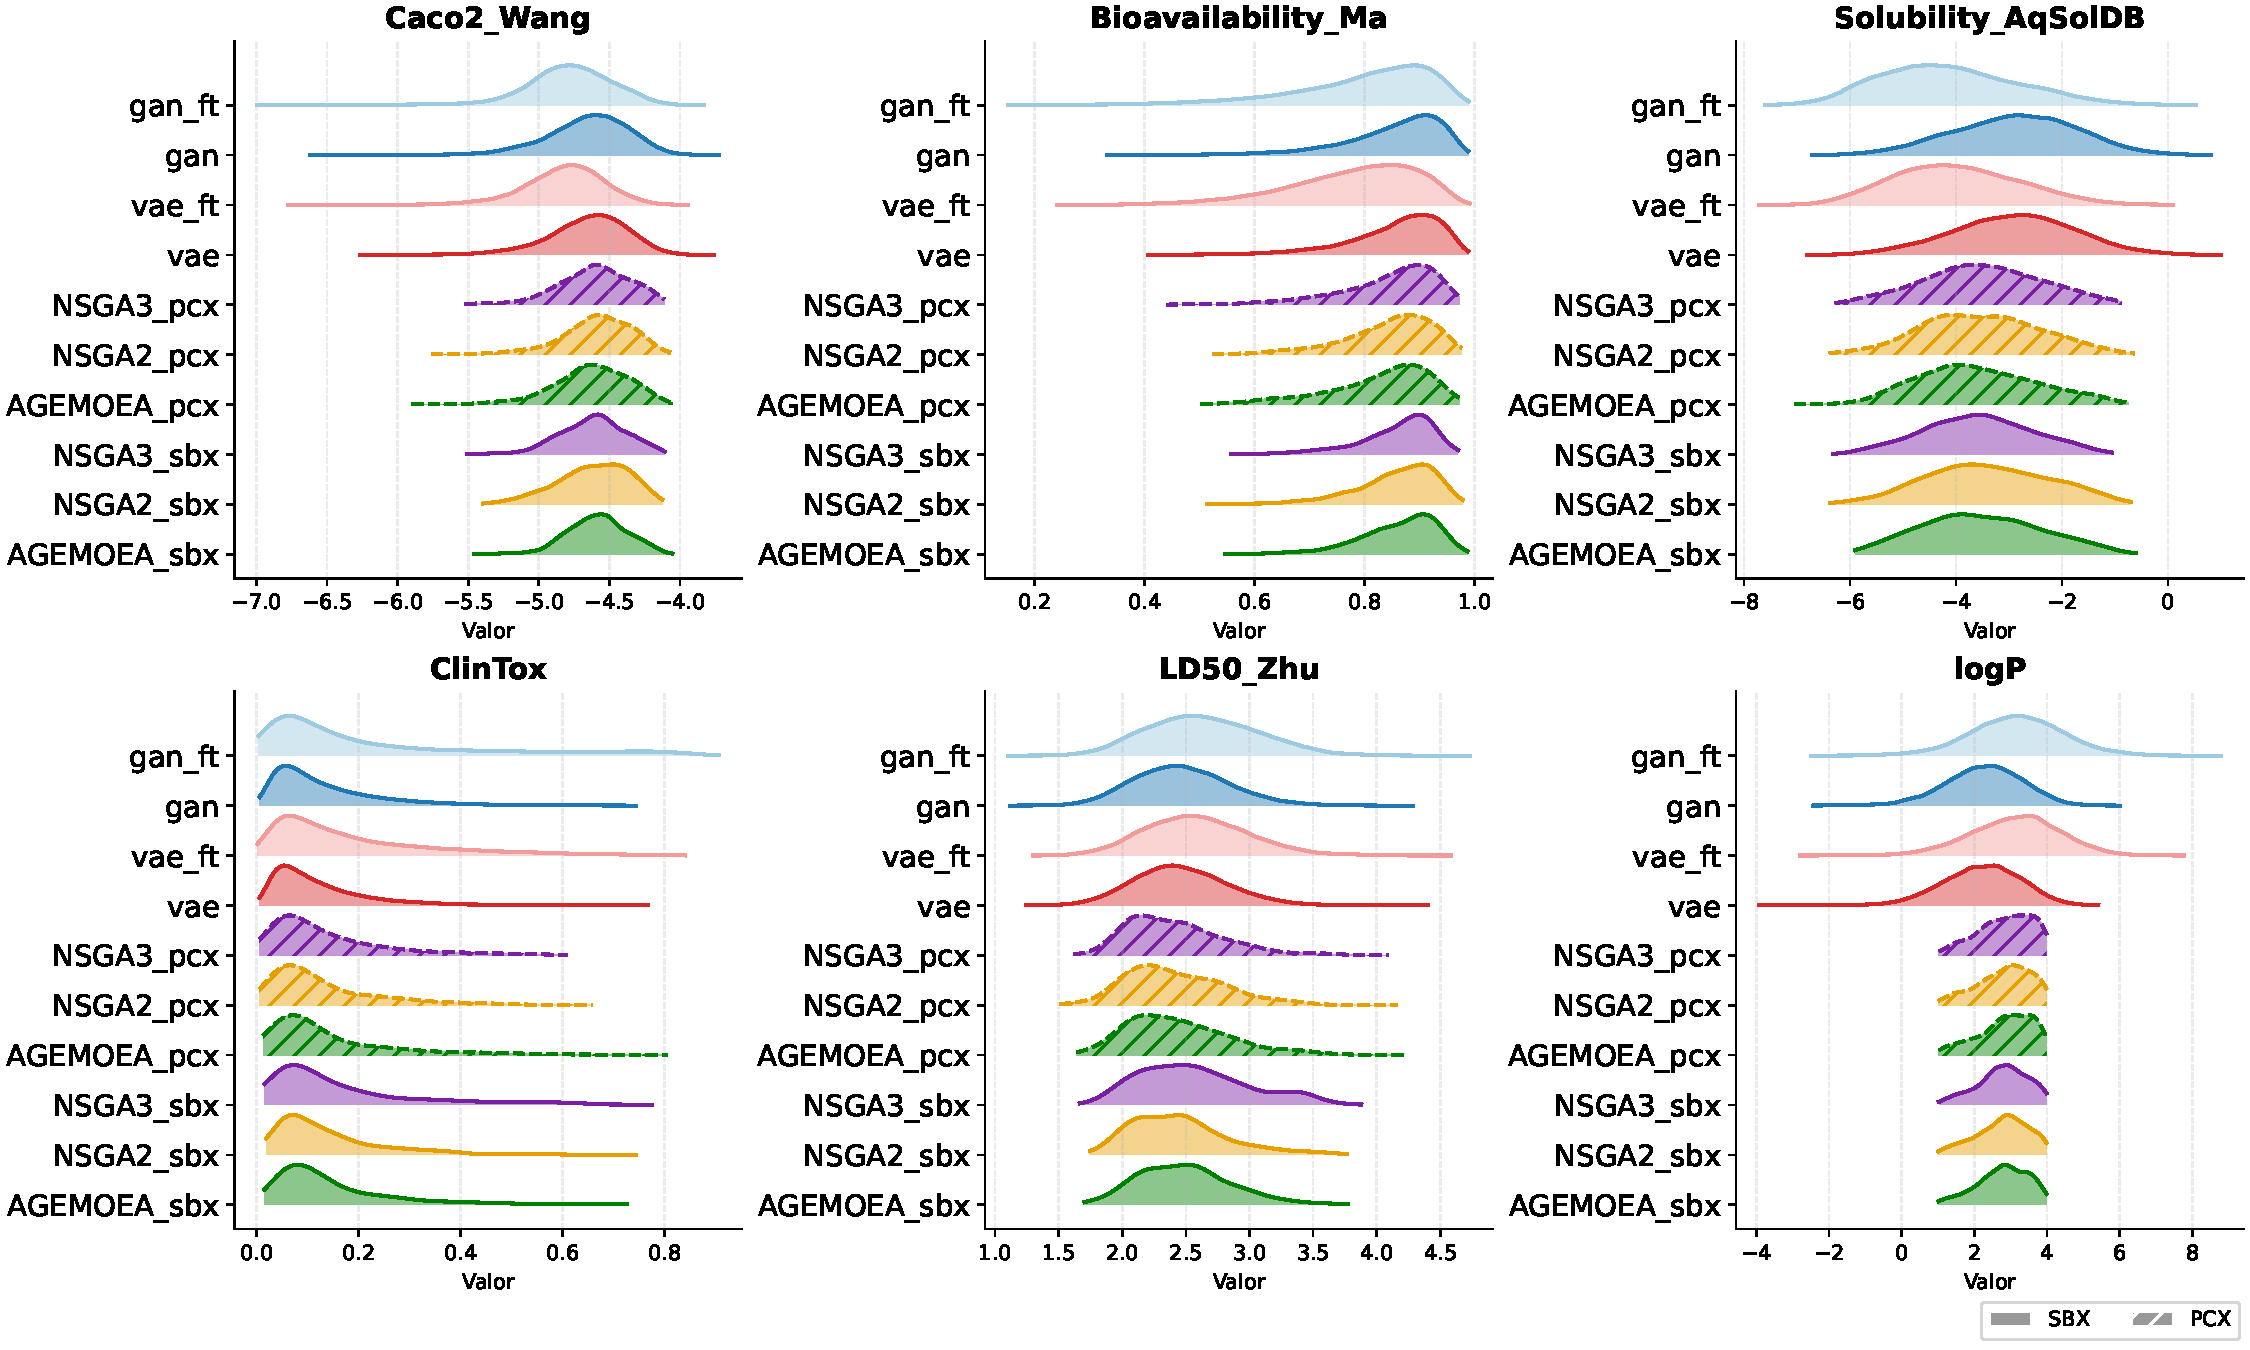
\includegraphics[width=0.98\textwidth]{Figures/mrp1/admet_ranks.pdf}
    \caption{Distribuciones de densidad (KDE) de las principales propiedades \gls{admet} predichas por ADMET-AI para cada algoritmo y modelo de referencia.}
    \label{fig:admet_ranks}
\end{figure}

\begin{table}[htbp]
\centering
\caption{Propiedades ADMET promedio predichas por ADMET-AI para cada configuración y modelo de referencia.}
\label{tab:admet_resumen}
\resizebox{\textwidth}{!}{
\begin{tabular}{lcccccccc}
\toprule
Configuración & HIA $\uparrow$ & Caco-2 $\uparrow$ & PAMPA $\uparrow$ & Biodisp. $\uparrow$ & Solubilidad $\uparrow$ & ClinTox $\downarrow$ & $\text{LD}_{50} \downarrow$ & $\log P$ \\
\midrule
NSGA-II (SBX) & $1.000$ & $-4.614$ & $0.950$ & $0.857$ & $-3.399$ & $0.139$ & $2.446$ & $2.775$ \\
NSGA-II (PCX) & $1.000$ & $-4.592$ & $0.948$ & $0.842$ & $-3.521$ & $0.132$ & $2.419$ & $2.825$ \\
NSGA-III (SBX) & $1.000$ & $-4.619$ & $0.949$ & $0.859$ & $-3.578$ & $0.164$ & $2.571$ & $2.784$ \\
NSGA-III (PCX) & $1.000$ & $-4.605$ & $0.949$ & $0.844$ & $-3.498$ & $0.136$ & $2.412$ & $2.862$ \\
AGE-MOEA (SBX) & $1.000$ & $-4.588$ & $0.952$ & $0.862$ & $-3.515$ & $0.145$ & $2.493$ & $2.799$ \\
AGE-MOEA (PCX) & $1.000$ & $-4.627$ & $0.948$ & $0.828$ & $-3.584$ & $0.142$ & $2.438$ & $2.868$ \\
\midrule
VAE & $0.999$ & $-4.652$ & $0.923$ & $0.855$ & $-2.907$ & $0.119$ & $2.460$ & $2.206$ \\
VAE-ft & $0.995$ & $-4.822$ & $0.894$ & $0.778$ & $-3.989$ & $0.185$ & $2.587$ & $3.120$ \\
GAN & $0.999$ & $-4.654$ & $0.921$ & $0.852$ & $-2.878$ & $0.131$ & $2.465$ & $2.264$ \\
GAN-ft & $0.996$ & $-4.786$ & $0.907$ & $0.794$ & $-4.137$ & $0.224$ & $2.640$ & $3.165$ \\
\bottomrule
\end{tabular}
}
\end{table}



La Figura~\ref{fig:admet_ranks} muestra las distribuciones de densidad KDE para los seis descriptores con mayor variabilidad (permeabilidad epitelial, biodisponibilidad oral, solubilidad acuosa, toxicidad clínica, toxicidad aguda y lipofilicidad), mientras que la Tabla~\ref{tab:admet_resumen} resume los valores medios de todas las propiedades \gls{admet} evaluadas (incluyendo la absorción intestinal humana HIA y la permeabilidad pasiva PAMPA):

\paragraph{Absorción y Permeabilidad.}
\begin{itemize}
    \item \textbf{Absorción Intestinal Humana (HIA\_Hou):} Estima la probabilidad de absorción oral (favorable $>0.8$). Todas las variantes multiobjetivo alcanzan valores óptimos de $1.0$, situándose ligeramente por encima de los modelos de referencia.
    \item \textbf{Permeabilidad Epitelial (Caco2\_Wang):} Mide la tasa de paso por células intestinales (alta permeabilidad $> -5.15$). Todas las variantes multiobjetivo se sitúan plenamente en la zona de permeabilidad alta, superando a los modelos ajustados por fine-tuning.
    \item \textbf{Permeabilidad Pasiva (PAMPA\_NCATS):} Evalúa el tránsito a través de membranas lipídicas (cruce óptimo $>0.70$). Las moléculas generadas presentan valores altos y homogéneos en todas las configuraciones, por encima de los modelos base y fine-tuning.
    \item \textbf{Biodisponibilidad Oral (Bioavailability\_Ma):} Probabilidad de alcanzar la circulación sistémica vía oral (favorable $>0.50$). Todas las configuraciones multiobjetivo logran promedios favorables, destacando \acrshort{agemoea} y \acrshort{nsga3} con SBX, y superando a los modelos con fine-tuning.
\end{itemize}

\paragraph{Propiedades Fisicoquímicas.}
\begin{itemize}
    \item \textbf{Solubilidad Acuosa (Solubility\_AqSolDB):} Expresada en $\log(\text{mol/L})$, donde valores entre $-4$ y $-2$ denotan solubilidad moderada y $<-4$ baja solubilidad. Las configuraciones multiobjetivo se mantienen dentro del rango moderado, con \acrshort{nsga2} (SBX) alcanzando la mejor solubilidad y evitando los valores deficientes observados en la GAN con fine-tuning.
    \item \textbf{Lipofilicidad ($\log P$):} Coeficiente de partición octanol/agua (rango ideal entre $0$ y $3$). Como resultado de la restricción aplicada, las moléculas optimizadas convergen de manera homogénea en valores cercanos a $2.8$, lo que favorece el cruce de membranas sin comprometer la solubilidad, a diferencia de los modelos con fine-tuning que superan el umbral recomendado.
\end{itemize}

\paragraph{Toxicidad y Seguridad.}
\begin{itemize}
    \item \textbf{Toxicidad Clínica (ClinTox):} Probabilidad estimada de fracaso o toxicidad en ensayos clínicos (perfil seguro $<0.30$). Las configuraciones multiobjetivo presentan probabilidades bajas de riesgo, destacando las variantes con PCX (en especial \acrshort{nsga2} y \acrshort{nsga3}) con los valores más seguros, mejorando consistentemente a los modelos con fine-tuning.
    \item \textbf{Toxicidad Aguda (LD50\_Zhu):} Dosis letal media en ratas expresada como $-\log(\text{mol/kg})$, donde valores más altos indican mayor toxicidad y el rango habitual oscila entre $2.0$ y $3.0$. Todas las variantes optimizadas se sitúan dentro de este intervalo habitual, con niveles comparables a los modelos generativos base.
\end{itemize}

% -----------------------------------------------------------------------------
\subsection{Discusión}
\label{subsec:discusion_mrp1}
\label{sec:discusion}

La formulación del diseño molecular optimizando simultáneamente la afinidad por acoplamiento en \gls{mrp1}, la potencia inhibitoria predicha pChEMBL, el \gls{qed} y la accesibilidad sintética SA, sujeta a restricciones de saturación ($F_{\text{sp3}}$) y lipofilicidad ($\log P$), permite orientar con éxito la exploración del espacio latente hacia regiones de interés biológico. En este entorno multiobjetivo con restricciones, el operador de cruce SBX ofrece un rendimiento superior a PCX. A diferencia de formulaciones más simples donde PCX favorecía la dispersión en zonas extremas, en este problema SBX preserva una validez química marcadamente más alta y alcanza mayores hipervolúmenes, lo que confirma que perturba en menor medida la coherencia estructural de los vectores latentes del \gls{vae}.

En la comparación entre algoritmos, los tres métodos muestran complementariedad al aportar soluciones al Frente No Dominado Conjunto Global. No obstante, \acrshort{nsga3} con SBX presenta el desempeño más consistente en la exploración de este espacio, alcanzando el mayor hipervolumen y el promedio más alto de pChEMBL. Esta ventaja se debe a que el uso de puntos de referencia estructurados en \acrshort{nsga3} guía la búsqueda de forma más equilibrada que la distancia de apiñamiento de \acrshort{nsga2} o la estimación geométrica de \acrshort{agemoea}, evitando el agrupamiento prematuro y logrando un balance favorable entre afinidad de unión, potencia y facilidad sintética.

Por otra parte, las pruebas con PoseBusters confirman que las poses generadas son físicamente viables y no presentan choques estéricos con \gls{mrp1}. Finalmente, al contrastar estos resultados con los modelos de referencia basados en ajuste fino (\textit{fine-tuning}), se evidencia la ventaja del enfoque propuesto: mientras que el \textit{fine-tuning} mejora la afinidad a expensas de degradar el \gls{qed}, empeorar la accesibilidad sintética y reducir drásticamente la validez química en modelos como la GAN, la optimización multiobjetivo en el espacio latente preserva la calidad molecular y asegura un perfil \gls{admet} favorable (alta absorción HIA, adecuada permeabilidad, lipofilicidad balanceada y menor riesgo en ClinTox), generando candidatos activos sin comprometer su viabilidad sintética ni farmacológica.

